\documentclass[12pt,oneside,a4paper,english]{article}

\usepackage{preamble}

\begin{document}

%\pagenumbering{Roman}
\pagestyle{empty}

\begin{titlepage}
\centering

\includegraphics[width=0.3\textwidth]{figures/root/dtu.png}
\vspace{3cm}


\hrule
\vspace{.5cm}
\huge{\textbf{Wi-Fi \& Satellite Scanner for Ultra-low Power Geolocation}} \\
\normalsize
\vspace{.5cm}
{ \Large \bfseries - Master Thesis -}
\vspace{.5cm}
\hrule
\vspace{2cm}

\textsc{\textbf{Author}}\\
\vspace{.5cm}
\centering
\authorNameA ~- \authorNumberA \\
\authorNameB ~- \authorNumberB

\vspace{1.5cm}
\centering

\vspace*{\fill} % Bottom of page
\centering June 20, 2024 %\today

\end{titlepage}


\newpage
\section*{Preface}
This thesis has been crafted over six months at the Department of Electrical and Photonics, at the Technical University of Denmark, as part of the master's degree in Autonomous Systems.

It is assumed that the reader has a basic knowledge in the areas of wireless communication \& embedded hardware and software design.
\newpage
\section*{Acknowledgements}
Thanks to
\newpage
%\begin{abstract}
%\end{abstract}\




\section*{Abstract}
abstract-text

\newpage

\tableofcontents
\addtocontents{toc}{\protect\thispagestyle{empty}}
\pagenumbering{gobble}
\newpage

\printacronyms[name={Abbreviations}]    % Will only print out if the acronym is used in the document. Dont put any \ac{} in captions of tables or figures if displaying a list of figures/tables, as the acronym will be displayed there first
\setcounter{table}{0}
\newpage

\listoffigures
\listoftables
\newpage

\pagestyle{fancy}
\pagenumbering{arabic}

\section{Introduction} \label{sec:introduction}
The ability to accurately determine the location of objects, assets, and individuals, in today's digital landscape, is paramount across a multitude of industries. From asset tracking in logistics to precision agriculture and smart city infrastructure, the demand for reliable geolocation solutions continues to grow. However, traditional methods of geolocation often face challenges such as limited coverage, susceptibility to signal interference, and high power consumption.

To address these challenges, our master thesis focuses on the development of a robust Geolocation System leveraging \ac{LoRaWAN}, Wi-Fi, and \ac{GNSS} technologies. By integrating these three complementary positioning systems, our solution aims to deliver precise location data while optimising power consumption for ultra-low power applications.

\ac{LoRaWAN}, with its long-range capabilities and low power requirements, serves as the backbone of our geolocation system, providing connectivity over extended distances with minimal energy consumption. Wi-Fi scanning augments this infrastructure by leveraging the ubiquitous presence of Wi-Fi networks in urban environments, enhancing localisation accuracy and coverage in indoor and dense urban areas where \ac{GNSS} signals may be obstructed. \ac{GNSS} further complements the system by providing global positioning capabilities, ensuring reliable outdoor localisation even in remote or \ac{GNSS}-challenged regions.


- Term of low power and ultra-low power. What's the difference
The definition of low-power and ultra-low power are


\subsection{Document structure}
What is the structure and what you can read in the different sections

Square brackets refer to hardware and software used for implementing the tracker with a red number (e.g.~\sbref{app:hardware:lr1110}). Applications and other references are referred in green by author and year in a square bracket (e.g. \cite{LR1110_user_manual})

Pin and ports of hardware are written in italics. The same goes with signals

\subsection{Product requirements}

Email, field trips, phone conversations, and company meetings have been the foundation for product requirements. The requirements are divided into technical details and design. The technical details are the most important foundation for the design requirements. The requirements are listed in tab.~\ref{tab:requirements}.

\begin{table}[H]
\centering
\caption{Product requirements.}
\begin{tabular}{c|p{7cm}p{6cm}}
\textbf{Category} & \textbf{Requirements} & \textbf{Wishes} \\ \hline
\multirow{18}{*}{\begin{tabular}[c]{@{}c@{}}Technical\\ detail\end{tabular}} 
    & \cellcolor[HTML]{EFEFEF}Class A as default & \cellcolor[HTML]{EFEFEF} \\
    & Location accessible by phone & Data accessed via our application \\
    & \cellcolor[HTML]{EFEFEF}\SI{10} - \SI{20}{\meter} uncertainty & \cellcolor[HTML]{EFEFEF}\SI{5} - \SI{10}{\meter} to prefer \\
    & Option to determine update interval & \\
    & \cellcolor[HTML]{EFEFEF}Range of \SI{5}{\kilo\meter} in open terrain & \cellcolor[HTML]{EFEFEF}\ac{SF} set by the user. Calculation of range and power consumption \\
    & Cold start-up time $\le$ \SI{15}{\second} & Better than the market \\
    & \cellcolor[HTML]{EFEFEF}Set update interval remotely & \cellcolor[HTML]{EFEFEF}\\
    & Ping interval minimum once an hour & Faster ping interval is better \\
    & \cellcolor[HTML]{EFEFEF}Locate inside and outside & \cellcolor[HTML]{EFEFEF}\\
    & Sleep consumption under \SI{0}{\milli\ampere} & \\
    & \cellcolor[HTML]{EFEFEF}Transmission consumption $\le$ \SI{0}{\milli\ampere} (default settings) & \cellcolor[HTML]{EFEFEF}\\
    & Low battery alarm & View battery percentage \\
    & \cellcolor[HTML]{EFEFEF}& \cellcolor[HTML]{EFEFEF}View temperature \\
    & & Battery can be recharged \\
    & \cellcolor[HTML]{EFEFEF}Location triggered by movement & \cellcolor[HTML]{EFEFEF} \\
    & Location triggered by no movement &  \\
    & \cellcolor[HTML]{EFEFEF} & \cellcolor[HTML]{EFEFEF}Geofence \\
    & 1000 positions on one battery charge & \\ 
\hline
\multirow{5}{*}{Design}
    & \cellcolor[HTML]{EFEFEF}Shape that enables easy case design & \cellcolor[HTML]{EFEFEF}\\
    & \SI{30}{\gram} with battery and without case & \\
    & \cellcolor[HTML]{EFEFEF}External antennas & \cellcolor[HTML]{EFEFEF}\\
    & Size: \si{5} $\times$ \si{4} $\times$ \SI{1.5}{\centi\meter} & \\
    & \cellcolor[HTML]{EFEFEF}Different battery configurations & \cellcolor[HTML]{EFEFEF}\\ 
\hline
\multirow{2}{*}{Other}
    & Open-source & \\
    & \cellcolor[HTML]{EFEFEF}Unit price $<$ \SI{1000}{\dkk} & \cellcolor[HTML]{EFEFEF}\\
\end{tabular}
\label{tab:requirements}
\end{table}

\newpage
\section{Development setup} \label{sec:dev-setup}
This section summarises guidelines for setting up an efficient developing environment for coding, flashing and debugging the STM32 chip using Visual Studio Code on both Linux and Windows. For a more elaborate guide see appendix \ref{app:devsetup}.

\subsection{Development prerequisites}
On both Windows and Linux start by cloning the code from GitHub: \url{https://github.com/MagnusErler/WiFiLocationTracker}

\textbf{Windows:}
If working on Windows\footnote{Windows Subsystem for Linux \ac{WSL} can not be used, as peripheral access (USB access) is not implemented in WSL2}, the following programs are needed:
\begin{itemize}
    \item CubeMX \sbref{app:software:stm32cubemx}
    \item OpenOCD \sbref{app:software:openocd}
    \item Visual Studio Code \sbref{app:software:vsc}
    \item Git (download as zip) \sbref{app:software:git}
    \item Arm GNU Toolchain (download as zip) \sbref{app:software:arm_toolchain}
    \item Package manager 
    \item Node.js
\end{itemize}

And the following binaries:
\begin{itemize}
    \item Make for Windows with dependencies \sbref{app:software:make}
\end{itemize}

\textbf{Linux:}
Suppose working on Linux CubeMX as needed. Maybe more.

software installations will be done through Linux's inbuilt package manager, and no program downloads are necessary.

\subsection{Installation guide}

\textbf{Windows:}
\begin{enumerate}
    \item Download all of the files, install VSCode and CubeMX and unpack the rest to a folder of your choice.
    \item Add paths for Arm GNU Toolchain, Make, OpenOCD and Git to system environment variables.
    \item Compile program using command \lstinline[style=bash]{make} in a terminal.
    \item Add openocd flash command to the newly created \lstinline[style=bash]{Makefile} using the stlink interface and with \textit{verify, reset, exit} as parameters.
 \end{enumerate}

\textbf{Linux:}
\begin{enumerate}
    \item Download and install CubeMX
\end{enumerate}
INDSÆT ENUMERATE OM HVORDAN MAN GØR PÅ LINUX

\subsection{Visual Studio Code integration}
This project's preferred \ac{IDE} is Visual Studio Code \sbref{app:software:vsc}. To integrate the project open the newly cloned repository and, if in Windows, run in the terminal \lstinline[style=bash]{wsl} to start performing like a Linux machine.

The compiling of the project is based on a simple makefile and can be compiled with:
\begin{lstlisting}[style=bash]
make
make -f CustomeNameMakefile     # used for custom names
\end{lstlisting}
If no error appears, a hex file is created inside the newly created folder (\lstinline[style=bash]{build\VSC_win.hex}) and can be flashed to the STM32 chip with \lstinline[style=bash]{make flash}.

For debugging, install Cortex-Debug \sbref{app:software:cortex_debug} in the Extension Marketplace.

Create a new folder called ".vscode" for personal setup of the debugging and running of the code and add two files from appendix \sbref{app:software:c_cpp_properties} and \sbref{app:software:launch}.

\subsubsection*{LoRaWAN setup?}
Skal man gøre noget, for at connect til LoRaWAN. Sætte account op eller noget?


Place modem firmware on the stm32 (\file{lr1110_updater_tool_v1.2.0_modem_v1.1.7.bin})


Then place the demo application (\file{lr1110_evk_v3.2.0.bin})


From https://github.com/Lora-net/SWTL001
Copy-paste firmware for transceiver on the STM32 by dragging the following .bin-file to the STM32 folder on your computer; \file{lr11xx-updater-tool_v2.3.0_lr1110_trx_0x0401.bin}

Then flash your application-code with Visual Studio Code.


Write down \lstinline[style=bash]{USER_LORAWAN_DEVICE_EUI}, \lstinline[style=bash]{USER_LORAWAN_JOIN_EUI}, and \lstinline[style=bash]{USER_LORAWAN_APP_KEY} (can be found on \url{Loracloud.com})

Run the following to update the alamanc; \lstinline[style=python]{python get_full_almanac.py -f almanac.h put_you_LoRaCloud_MGS_token_here}
Find the token on \url{loracloud.com}
and then make and flash the bin-file to the board: \lstinline[style=bash]{make full_lr1110 MODEM_APP=EXAMPLE_FULL_ALMANAC_UPDATE}


%https://www.youtube.com/watch?v=xaC5oWwzOt0&t=6s

Serial monitor in terminal: \lstinline[style=bash]{cu -l /dev/ttyACM0 -s 115200} (find your port with \lstinline[style=bash]{ls /dev/tty*}).

\url{https://www.loracloud.com/portal/modem_services/home}
Join server -> Devices -> "insert pin and get" -> Export device keys -> Choose "LoRaWAN version 1.0.3"


JOIN\_EUI - (8 bytes):
 00 16 C0 01 FF FE 00 01
CHIP\_EUI - (8 bytes):
 00 16 C0 01 F0 1A 33 DF
CHIP\_PIN - (4 bytes):
 BF 21 77 43
 
 
\url{https://js.loracloud.com:7009}
\newpage
\section{State of the art} \label{sec:knowledge}
This section overviews the foundational knowledge vital for developing a product with the LR1110 chip. It aims to establish a solid understanding of the project's infrastructure and technologies, equipping the reader with the necessary tools and knowledge to work with the LR1110 effectively, and succinctly describe the used product design methodologies. 

\subsection{Communications protocols}
\subsubsection{Serial communication}
Serial communication is a broad term that refers to any form of data transmission in which bits are sent sequentially, one after the other, over a single communication channel, which encompasses various serial communication methods, including \ac{I2C}, \ac{USART}, \ac{SPI} and others. These methods may differ in protocol, hardware requirements, speed, and application.

\subsubsubsection*{Universal Synchronous and Asynchronous Receiver/Transmitter (USART)}
\ac{USART}, is a half-duplex, asynchronous interface, and a widely used serial communication interface employed in microcontrollers, embedded systems, and various electronic devices. \ac{USART} enables asynchronous, non-simultaneous (half-duplex) data transmission between devices via dedicated TX and RX lines and a shared ground without a shared clock signal. This allows for greater flexibility in communication between devices operating at different speeds and with varying clock characteristics. Moreover, its asynchronous operation simplifies hardware implementation, promotes cross-platform compatibility, and renders it cost-effective and straightforward to deploy \cite{UART1}, \cite{UART2}.

\subsubsubsection*{Serial Peripheral Interface (SPI)}
\ac{SPI} is a full-duplex, synchronous interface, and one of the most widely used between microcontroller and peripheral ICs such as sensors, ADCs, DACs, shift registers, SRAM, and others. It operates on a master-slave model, on a four-wire configuration, encompassing shared \ac{MOSI}, \ac{MISO}, and \ac{SCK} lines, complemented by individual \ac{SS} lines for each distinct device in a multi-slave environment.

Distinguished from the asynchronous nature of \ac{USART}, \ac{SPI}'s synchronous operation is characterised by using dedicated data lines alongside a clock signal to maintain synchronisation between transmitting and receiving entities. This synchronisation ensures precise timing for data exchange, enhancing communication reliability and efficiency, negating the overhead stemming from including start and stop bits with each transmitted byte, and the susceptibility to data corruption in mismatched baud rates between communicating devices.
Further differentiating \ac{SPI} is its full-duplex capability, which permits simultaneous transmission and reception of data, thereby optimising throughput and enhancing efficiency in data exchange.

Compared to \ac{USART}, \ac{SPI} boasts superior speed and supports multiple peripherals. However it still requires more signal lines (wires) than other communications methods, as each peripheral requires a \ac{SS} line, and communication remains centralised under the master device, precluding direct communication between peripheral devices \cite{SPI_analog}, \cite{SPI_sparkfun}, \cite{SPI_wiki}.

\subsubsection{Wi-Fi}
Wi-Fi is a part of a wireless network protocol based on the technical standard IEEE 802.11\footnote{\url{https://www.ieee802.org/11/}}. For most people, Wi-Fi is synonymous with wireless internet access. However, the LR1110 chip does not use Wi-Fi in its conventional role as a data conduit. Instead, it serves as a tool for geolocation through Wi-Fi sniffing, harnessing access point signals to determine the device location. This method is explained in section %\ref{indsæt ref}

\subsubsection{Global Navigation Satellite System (GNSS)}
\ac{GNSS} is the general term for any satellite constellations that orbit the Earth and provides radio-based positioning, navigation, and timing information to users worldwide. This information can be used for trilateration; determining the unknown position coordinates of a point of interest, which is described in section %\ref{indsæt ref}.
The most well-known constellation is the United States-operated \ac{GPS} \ac{GPS}. Other constellations are GLONASS from Russia, Galileo from the European Union, BeiDou from China, IRNSS from India and QZSS from Japan. The LR1110 chip is capable of receiving signals from both GPS and BeiDou satellites.
Because of the signal strength and distance to the satellites, geopositioning using GNSS is predominantly viable in outdoor environments.

More information about GNSS, if we need to write more:
\url{https://www.youtube.com/watch?v=FU_pY2sTwTA}
\url{https://www.youtube.com/watch?v=wCcARVbL_Dk}

%GNSS ID\\
%\ac{C/N0} is a metric used to quantify the strength of a satellite signal relative to the background noise in the receiver's environment. \ac{C/N0} is often expressed in decibels [\si{\dB}] and is a crucial parameter in determining the quality of the received satellite signal. A higher \ac{C/N0} value generally indicates a stronger and more reliable satellite signal, which is desirable for accurate positioning and navigation.

\subsubsection{Long Range/Wide-Area-Network (LoRa/LoRaWAN)}
\ac{LoRa}, is an open standard,  networking layer, that is particularly well-suited for the \ac{IOT} and other applications where devices need to transmit small amounts of data over long distances while operating on low power \cite{LoRaWAN_1_0}. \\

As shown in figure \ref{fig:LoRa_bandwidth_range} other \ac{LPWAN} technologies exist, however as \ac{LoRa} is the only protocol the LR1110-chip implements at this point, it is chosen wireless communication protocol for this project.
Considerations around the communication protocol and the advantages and disadvantages of \ac{LoRa} versus protocols with similar purposes will be presented in section \textcolor{red}{indsæt reference}.

\begin{figure}[H]
    \centering
    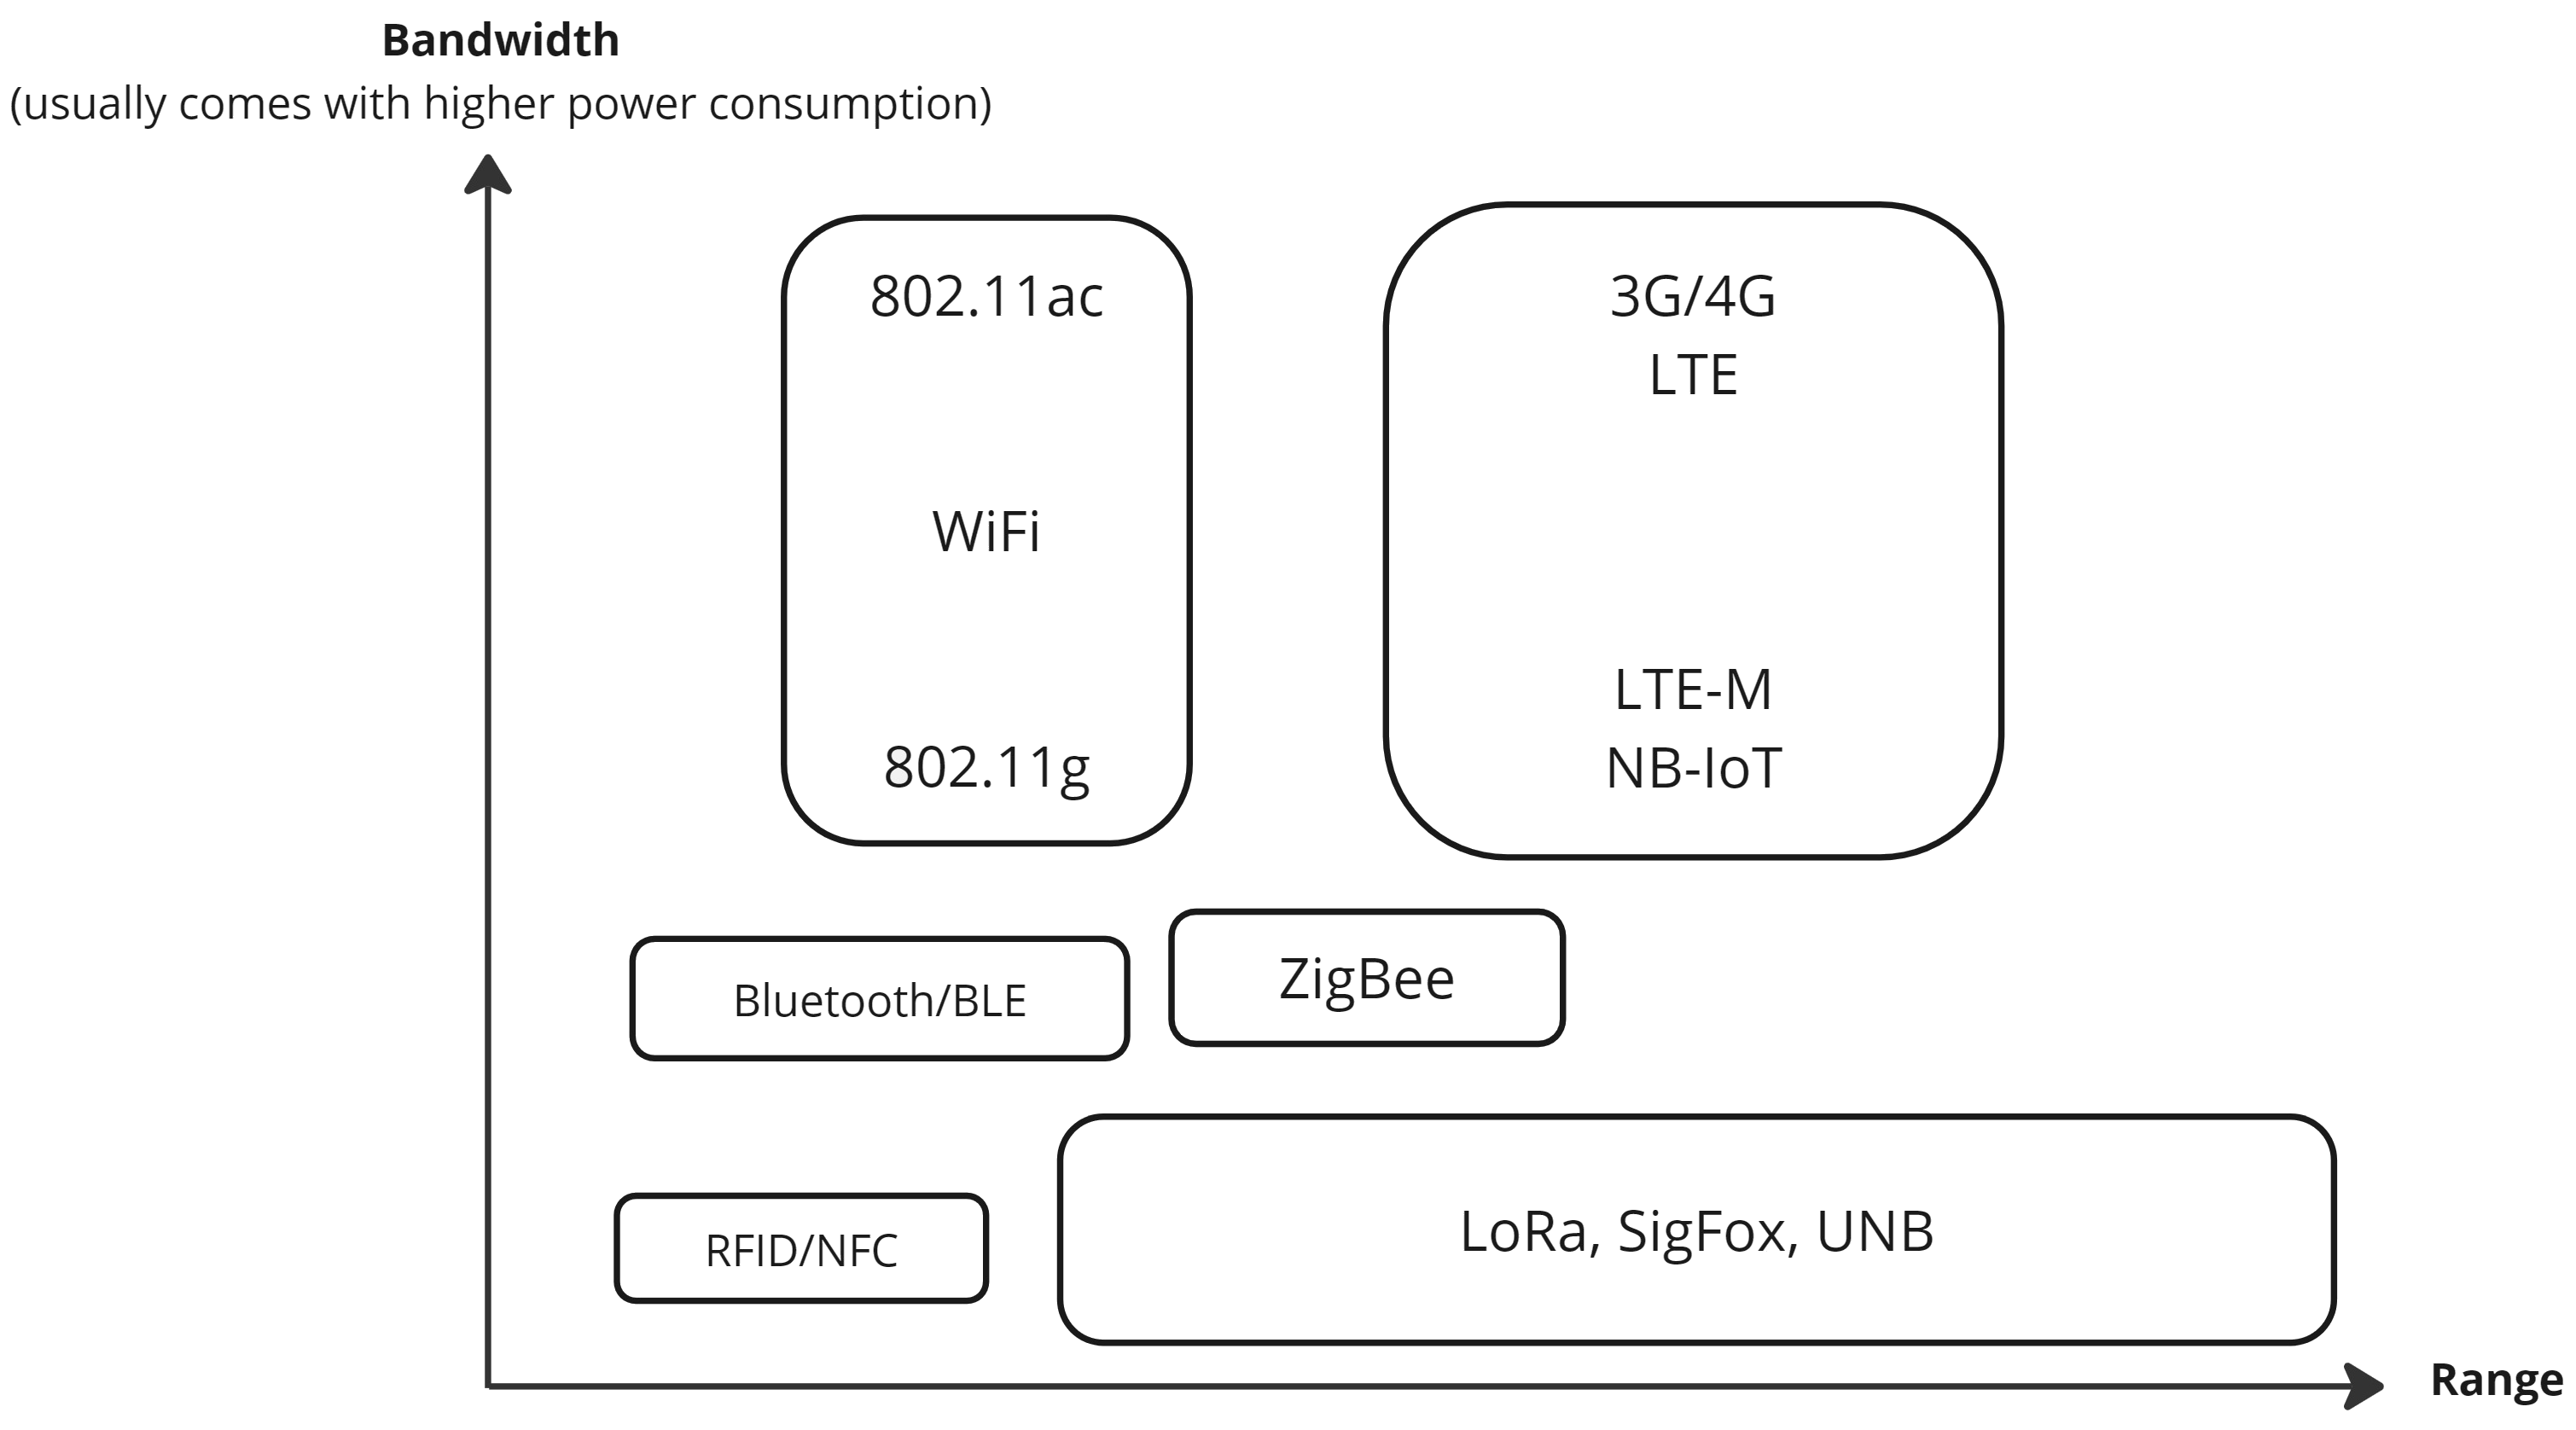
\includegraphics[width=0.8\textwidth]{figures/range_bandwidth.png}
    \caption{Plot showing bandwidth versus the range of different wireless communication technologies. Rework from: \url{https://www3.cs.stonybrook.edu/~mdasari/courses/cse570/lora.pdf}}
    \label{fig:LoRa_bandwidth_range}
\end{figure}

\subsubsubsection*{En overskrift}
\ac{LoRa} refers to the physical layer and the proprietary spread spectrum modulation technique developed by Semtech, while \ac{LoRaWAN} refers to the network layer that defines the communication protocol and system architecture, enabling devices to communicate with \ac{LoRa} gateways and network servers. \ac{LoRaWAN} specifies how data should be transmitted, how end devices authenticate themselves on the network, how messages are acknowledged, and how devices can go into low-power sleep mode to conserve energy.

\ac{LoRaWAN} supports different classes of devices, allowing for flexibility in applications requiring either periodic or event-driven data transmission.

\ac{DevEUI} (also known as ChipEUI) is like a \ac{MAC} address, a unique identifier for the device. It is a 64-bit number that is assigned to the device by the manufacturer. The \ac{DevEUI} is used to identify the device in the network and is used in the activation process. \ac{JoinEUI} (also known as AppEUI) is a 64-bit number that is used to identify the network server in the activation process. The \ac{AppKey} is a 128-bit number that is used to encrypt the messages between the device and the network server. The \ac{AppKey} is used in the activation process to derive the \ac{NwkSKey} and \ac{AppSKey}.


%https://www.loracloud.com/documentation/join_service?url=glossary.html#term-Join-Server

Fig.~\ref{fig:LoRa_bandwidth_range} shows the difference between Wi-Fi and \ac{BLE}, versus \ac{LoRa} and cellular signals, comparing the range of the signal travelling and the bandwidth of the signal.

\ac{LoRaWAN} communicates on different frequencies depending on where the device is located; EU: \SI{868}{\mega\hertz} and \SI{433}{\mega\hertz}, US: \SI{915}{\mega\hertz}, AS: \SI{430}{\mega\hertz}.

SKRIV OGSÅ OM PRIS OG GATEWAYS PÅ LORAWAN
Evt.indsæt billede af Topology. End nodes <-> Gateways (private or corporate) <-> Network server <-> Application server

\ac{SF}

\subsubsection{HTTP/REST API}
Måske vil skal skrive noget om dette

\subsection{The LoRaCloud ecosystem}
Join server
Modem \& geolocation services

\subsection{Geopositioning}
Geopositioning or geolocation is the process of determining or estimating the geographic position of an object \cite{ISO19130}. This can be done using many different methods, each with strengths and weaknesses regarding workload and accuracy. This thesis focuses on using Wi-Fi and \ac{GNSS} combined with Google\footnote{Google Geolocation API: \hangindent=2em \url{https://developers.google.com/maps/documentation/geolocation/overview}} and Semtechs Geolocation APIs \footnote{LoRa Cloud: \url{https://www.loracloud.com/}} to get a general location of the LR1110 chip.

%https://lora-developers.semtech.com/learn/hands-on-labs/build-end-to-end-solution-using-lorawan-and-loraedge/find-the-location-of-your-tracking-device/


"Google's Geolocation API is a service provided by Google that allows developers to retrieve the approximate geographical location of a device based on various factors, without necessarily relying on \ac{GPS}. Here's a basic overview of how it works:

\textbf{Request Submission}: The client (a web browser or a mobile app) sends a request to the Geolocation API endpoint with data about nearby Wi-Fi access points, cellular towers, or Bluetooth beacons that the device can detect. This data includes information like the \ac{MAC} addresses of Wi-Fi access points, cell tower IDs, signal strengths, and other relevant parameters.

\textbf{Data Processing}: Google's servers receive the request and analyse the data provided. They compare the received data against a vast database of known Wi-Fi access points, cell tower locations, and their corresponding geographical coordinates. Google continuously collects this data through its Street View cars, mobile mapping vans, and other sources, building a massive database of Wi-Fi and cell tower locations worldwide.

\textbf{Triangulation and Trilateration}: Using the information gathered from nearby Wi-Fi access points, cellular towers, and other available signals, Google's servers apply techniques like triangulation and trilateration to estimate the device's location. Triangulation involves determining the device's position by measuring the angles between it and known points (e.g., Wi-Fi access points). Trilateration involves calculating the device's position based on its distance from multiple known points.

\textbf{Response}: After processing the request and estimating the device's location, the Geolocation API returns a response containing the latitude and longitude coordinates of the device's approximate location. Additionally, the response may include other information such as the accuracy of the location estimate and a confidence radius.

\textbf{Privacy Considerations}: Google takes privacy seriously and implements measures to protect user privacy when using the Geolocation API. For example, the \ac{API} may not return precise location data in certain cases, and users have control over their location-sharing settings through their device settings and Google account preferences.

Overall, Google's Geolocation API provides a convenient and efficient way for developers to determine the approximate geographical location of a device without relying solely on \ac{GPS}, making it useful for a wide range of location-based applications and services."

%https://samy.pl/mapxss/
%https://developers.google.com/maps/documentation/geolocation/overview
%https://blog.invgate.com/how-to-locate-a-device-using-a-mac-address
%https://blog.semtech.com/indoor-wi-fi-geolocation-with-lora-edge
%https://lora-developers.semtech.com/community/faq/faq-geo-location
%https://lora-developers.semtech.com/learn/hands-on-labs/build-end-to-end-solution-using-lorawan-and-loraedge/find-the-location-of-your-tracking-device/

\subsubsection{GNSS positioning}

The LR1110 features a fast and low-power \ac{GNSS} scanner. The device captures a short portion of the signal broadcast by the
\ac{GNSS} satellites and extracts the information required to calculate the device position - the pseudo ranges. This information is aggregated into a \ac{NAV} which can be sent to a solver to compute the device position.

\begin{figure}[H]
    \centering
    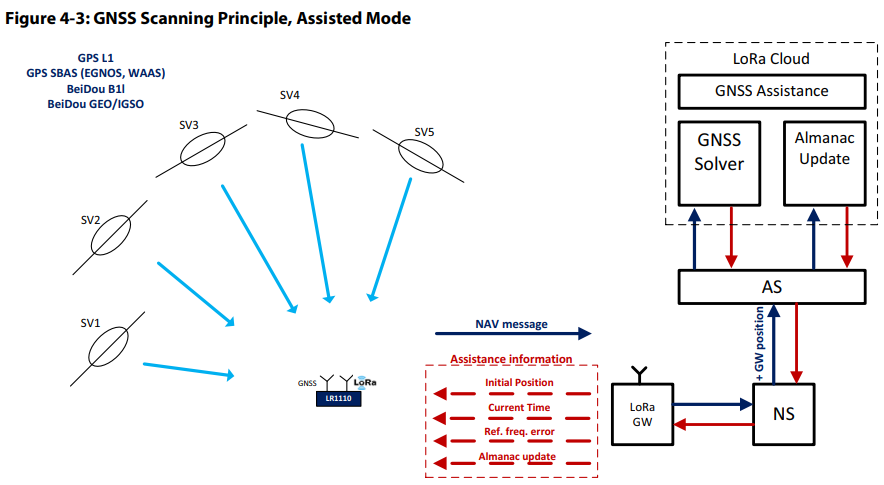
\includegraphics[width=0.9\textwidth]{figures/GNSS_scanning.png}
    \caption{GNSS Scanning Principle, Assisted Mode.}
    \label{fig:gnss_scanning}
\end{figure}
% taken from: https://semtech.my.salesforce.com/sfc/p/#E0000000JelG/a/3n000000vBus/cPXIY7jwqFWpmW7USMtfqpJt7T5afR439wbYefi4tsI page 17

Providing assistance information to the LR1110 will minimize the search space, reducing the capture time and the energy spent.

The \ac{GNSS} scanner of the LR1110 has two modes of operation: autonomous and assisted.

\subsubsubsection{Autonomous GNSS Scanning}
The LR1110 will not require any assistance information in this mode. A fast search of all \ac{SV}s with strong signals in the
selected constellation is performed, and all the \ac{SV}s received with a signal better than RXSGPS1E\footnote{RXSGPS1E: GPS, indoor classification, and strong signal SV capture. Typ. \SI{-134}{\dB}\cite{LR1110_datasheet}} are detected.
This mode can be used to determine if the device stands indoors or outdoors; in case no \ac{SV} with a strong signal is detected, the application concludes that the device is indoors. Therefore the search for weak signals, which takes more time and energy, can be discarded; the search for other signals of opportunity, like Wi-Fi, might be launched instead.

\subsubsubsection{Assisted GNSS Scanning}
Based on the assistance information, the LR1110 will build a list of 10 to 12 \ac{SV}s that it should look for at the position of the device and the actual time.
Two different assisted \ac{GNSS} scanning modes are implemented:
\begin{itemize}
\item \textbf{Low power}: A first search of strong signal satellites within the list of visible ones will be made. If at least one satellite is found in this step, the search will continue for satellites with weaker signals. Otherwise, the search will stop. This mode minimises energy consumption and can also be used as an indoor/ outdoor detection method, in a more efficient way than the autonomous \ac{GNSS} scanning mode. The indoor classification is decided after searching 10-12 \ac{SV}s, versus 32-35 in Autonomous scanning mode.
\item \textbf{Best effort}: A first search of \ac{SV}s with strong signals, within the list of visible satellites, is made. Even if no satellite is found in the first phase, the search continues for satellites with weaker signals. This mode is to be used in difficult environments where it may be possible to find \ac{SV}s, at the expense of a longer search phase.
\end{itemize}
The scanner uses a sequence of capture and processing phases. To reserve power, the \ac{RF} front end will be turned off during the processing phases.

\subsubsection{Wi-Fi positioning/Geolocation databases/API}
Semtech
Google
Apple, Qualcomm, Wiggle

\subsection{Product design}
A brief introduction to what product design is. Maybe how it has changed?

\subsubsection{Prototyping}




3D-printing
However, since interactive systems are complex, it may be difficult or impossible to create prototypes of a whole design in the formative stages of a project.
Choosing the right kind of more focused prototype to build is an art in itself, and communicating its limited purposes to its various audiences is a critical aspect of its use

This chapter aims to establish a model that describes any prototype in terms of the artifact being designed, rather than the prototype's incidental attributes. By focusing on the purpose of the prototype—that is, on what it prototypes

Prototypes provide the means for examining design problems and evaluating solutions. Selecting the focus of a prototype is the art of identifying the most important open design questions

Teksten ovenfra er fra Houde - What do Prototypes prototype?
Skriv om, hvordan prototyper kan teste forskellige ting, og hvordan opmærksomhed på dette inden, kan hjælpe med at få det rigtige udkom af ens prototype.

\subsubsection{Actor-oriented design}
Hvad er en fælles nævner for de forskellige etnografiske feltstudiemetoder?
Det er kvalitativ metode eftersom at dette er essentielt for design, da vi er interesserede i detaljer!

Hvad er induktiv tilgang?
Empirisk induktiv. Man starter med kvalitativ dataindsamling, man finder heraf en induktiv slutning og ser heraf en sammenhæng eller et mønster.
Fx. I et givet tidsrum på et bestemt sted er alle fugle sorte, og man konkluderer heraf at alle fugle er sorte

Hvad er Grounded Theory, samt hvilken tilgang?
Induktiv. En design-ingeniørs måde hvorpå at være undersøgende og starte fra bunden -> vi starter i empirien.
Problemet defineres på baggrund af den data der indsamles. En analyse kan vise mønstre af tematikker.

Hvad hører sammen med kvalitativ data?
Induktiv! Videnskabelig metode som ikke er målbar.

Interviews - Etnografisk felstudie
Hvad er en fælles nævner for de forskellige etnografiske feltstudiemetoder?
Det er kvalitativ metode eftersom at dette er essentielt for design, da vi er interesserede i detaljer!

Hvilken tilgang skal vi helst bruge som design-ingeniører? - Induktiv

Hvad er et etnografisk interview?
Det er en kvalitativ metode.
Et åbent interview hvor man kommer tættere på aktørens kultur og praksis.
Man gør sig fremmed for det felt man undersøger.
Iterativt -> kræver en analyse som ofte leder op til et nyt feltbesøg.

Hvad skal man have med når man forbereder sig til interviews?
Hvilken viden mangler vi?
Hvem ligger inde med den?
Hvem tager vi kontakt til? Hvordan tager vi kontakten?
Hvem faciliterer interviewet?
Hvordan dokumenterer vi undervejs?
Hvor udfører vi interviewet? (on location eller ....?)
Hvordan deler vi viden efterfølgende (optager vi samtalen, skriver vi noter, laver vi arbejdsblade?)

Hvad er et affinitetsdiagram, overordnet?
At gruppere viden (KJ-metoden)
Deling af viden i teamet, fra forskellige kilder.
Fortolkning af viden, analyse.

Skriv ting på post-its og grupper efterfølgende i overordnede temaer.

Hvad tager affinitetsdiagrammer udgangspunkt i?
Grounded theory; derfor, lad empirien tale -vundgå prædefinerede kategorier.
Start med statements/findings og IKKE med overskrifterne.

\subsubsection{Design criteria}
How to set up design criteria.
Here, we must talk about requirements, criteria and wishes.
Requirements are things that must be
Criteria are measurable. This means that they can be more or less fulfilled.
Wishes are nice to have

\subsubsection{Use cases}
How do you find use cases? What are use cases?

\subsubsection{Affinity diagram/KJ-method}
Affinity: a similarity of characteristics suggesting a relationship, especially a resemblance in structures and thoughts.
Affinity mapping gives designers a visual view of their research, capturing data so that themes, trends, and needs emerge.
Affinity mapping is done during the divergent research phase. In this diagram of the Double Diamond, where the first diamond to the left represents research discovery and analysis, affinity mapping can be done multiple times to organise and analyse research data. At the beginning of the design phase, represented by the second diamond on the right, research should be finalised. It is not recommended to do affinity mapping during the design phase.
\newpage
\section{System/Product design} \label{sec:design}
This section dives into the tracker's design, starting with establishing product requirements using an actor-oriented approach and addressing the \ac{PCB} design and case design for optimal functionality and user experience.
In between this, the implementation of software features and strategies for power minimisation to enhance battery life will be explored

\subsection{Development of product requirements}
\textit{The following section is a rough draft}
There are many different ways to go about product development and many different ways to get a design assignment. You can be assigned to design a product where the goals have been clearly defined in advance by others, you can be tasked with redesigning an already existing product with all of its inherent product requirements, you can get tasked to design a product for a client who most likely has thoughts, ideas and wants for that, or in our case, have a broad idea that you are trying to turn into a product.

One way to start developing product requirements for such a task is to think about use cases to look into competitors on the market, and compare their features, to get an idea if there is an opening in the market, and if not which requirements your product should have, to be able to compete against similar products.

On the market today, there are two major technologies for tracking objects: \ac{GPS} trackers and Bluetooth trackers.
\ac{GPS} trackers work individually and utilise the \ac{GNSS} network to track the position of the object, and then use \ac{GSM} or an \ac{LPWAN} like \ac{LoRaWAN} or Sigfox to broadcast the location.
Bluetooth trackers on the other hand connect to your or nearby phones and then use the phone's location and data connection, to broadcast its location.


% STORK: https://tektelic.com/wp-content/uploads/STORK-Asset-Tracker.pdf

The most popular Bluetooth trackers are the Apple AirTag\footnote{\url{https://www.apple.com/airtag/}} and Tile.
Pros:
\begin{itemize}
  \item Compact and Lightweight: Most Bluetooth trackers are small and lightweight, making them easy to attach to various items without adding bulk or weight.
  \item Affordable: Bluetooth trackers are generally more affordable than \ac{GPS} trackers, making them accessible to many users.
  \item Long Battery Life: Many Bluetooth trackers come with replaceable batteries that last several months or even years, ensuring prolonged usability without frequent recharging.
  \item Can use \ac{UWB} for really precise close-by tracking.
\end{itemize}

Cons:
\begin{itemize}
  \item Limited Range: Bluetooth trackers have a limited range compared to \ac{GPS} trackers, typically around 100-200 feet indoors and up to 300 feet outdoors, which may restrict their effectiveness in certain situations.
  \item Dependency on Smartphone: Bluetooth trackers rely on the connection to a smartphone or tablet via Bluetooth, so if the smartphone's battery dies or Bluetooth is turned off, tracking functionality may be compromised.
  \item Lack of \ac{GPS}: Unlike \ac{GPS} trackers, Bluetooth trackers do not provide real-time location updates or tracking over long distances, limiting their usefulness for locating items beyond the Bluetooth range.
  \item Vendor-specific: Bluetooth trackers are often designed to work exclusively with devices from a specific manufacturer or ecosystem. For example, Apple's AirTag is optimised for iPhone use and relies on the Find My app, while other Bluetooth trackers may be tailored for Android devices or specific third-party platforms. This vendor specificity limits cross-platform compatibility and may exclude users who do not use compatible devices, reducing the overall accessibility and interoperability of Bluetooth trackers.
\end{itemize}

Pros and cons of \ac{GPS} trackers:\\
Pros:
\begin{itemize}
  \item Accurate Tracking: \ac{GPS} trackers provide real-time and precise location data, allowing users to monitor the exact whereabouts of their belongings or vehicles.
  \item Long-Distance Coverage: \ac{GPS} trackers can track items over long distances, making them suitable for locating assets that may travel far from their original location.
  \item Wide Compatibility: \ac{GPS} trackers are generally compatible with various devices and platforms, offering broader accessibility to users regardless of their preferred devices or ecosystems.
  \item Geofencing Capabilities: Many \ac{GPS} trackers offer geofencing features, enabling users to set virtual boundaries and receive alerts when their tracked items enter or exit designated areas.
\end{itemize}

Cons:
\begin{itemize}
  \item Subscription Fees: Some \ac{GPS} trackers require subscription plans for accessing features like real-time tracking or historical data, adding ongoing costs for users beyond the initial purchase price.
  \item Power Consumption: \ac{GPS} trackers often consume more power than Bluetooth trackers, leading to shorter battery life or the need for frequent recharging.
  \item Reliance on Satellite Signals: \ac{GPS} trackers rely on satellite signals for location tracking, which may be obstructed or limited in certain environments such as indoors or urban areas with tall buildings, reducing tracking accuracy or effectiveness.
  \item Higher Cost: \ac{GPS} trackers tend to be more expensive than Bluetooth trackers due to their advanced features and capabilities, potentially making them less accessible to budget-conscious users.
\end{itemize}

\begin{table}[H]
\scriptsize
\caption{Other tracker}
\label{tab:other_tracker}
\begin{tabular}{llllllp{3cm}}
 & Price & Size [mm] & Battery & Mont. cost & Track. dist. & Features \\
\hline
Apple AirTag & 300 & $32 \times 32 \times 8$ & Up to 1 yr & Free & \SI{30}{\meter} & \ac{BLE}, speaker, many\newline people own iPhones \\
\makecell[l]{Tile mate\\\,} & \makecell[l]{>260\\\,} & \makecell[l]{$38 \times 38 \times 7$\\\,} & \makecell[l]{Up to 1 yr\\\,} & \makecell[l]{Free\\\,} & \makecell[l]{\SI{76}{\meter}\\\,} & Watertight (IP67), different forms, speaker \\
\makecell[l]{MiniFinder Pico\\\,} & \makecell[l]{2950\\\,} & \makecell[l]{$61 \times 41 \times 16$\\\,} & \makecell[l]{40 h (5 min interv.),\\20 days (standby)} &  &  &  \\
\makecell[l]{MiniFinder nano\\\,} & \makecell[l]{3000\\\,} & \makecell[l]{$47 \times 41 \times 16$\\\,} & \makecell[l]{36 h active,\\ 120 h stand-by} &  &  &  \\
Minifinder Extreme & 3600 & \makecell[l]{$88 \times 62 \times 34$\\} & 10 yr (standby) &  &  &  \\
Cobblestone Pro & 1500 & \makecell[l]{$64 \times 64 \times 23$\\} & 4 yr (1 update/day) & Free &  &  \\
Zmartgear Sigfox & 1300 & \makecell[l]{$42 \times 24 \times 17$\\} & 3 months (standby) & 3 yr free &  &  \\
Odin tracker & 2500 & \makecell[l]{$58 \times 41 \times 19$\\} & 10 yr (3000 tracks) & 0 &  &  \\
\end{tabular}
\end{table}

\iffalse
\textbf{Popular trackers:}\\
\textbf{Apple AirTag} (\ac{BLE})
\begin{itemize}[label={}, noitemsep, leftmargin=0pt]
    \item Price: \SI{300}{\dkk}
    \item Size: \si{31,9} × \si{31,9} × \SI{8}{\milli\meter}
    \item Battery life: Up to 1 year
    \item Monthly cost: Free
    \item Tracking distance: \SI{30}{\meter}
    \item Other notable features: \ac{UWB}, speaker, many people own iPhones
\end{itemize}

\textbf{Tile mate} (Bluetooth)
\begin{itemize}[label={}, noitemsep, leftmargin=0pt]
    \item Price: from \SI{260}{\dkk}
    \item Size: \si{37,8} × \si{37,8} × \SI{7.2}{\milli\meter}
    \item Battery life: Up to 1 year
    \item Monthly cost: Free
    \item Tracking distance: \SI{76}{\meter}
    \item Other notable features: speaker, can be bought in different forms, watertight (IP67)
\end{itemize}

\textbf{MiniFinder Pico} (\ac{GPS})
\begin{itemize}[label={}, noitemsep, leftmargin=0pt]
    \item Price: \SI{2950}{\dkk}
    \item Size: \si{61} × \si{41} × \SI{16}{\milli\meter}
    \item Battery life: \si{36}-\SI{40}{\hour} with \SI{5}{\minute} intervals, 20 days on standby
    \item Weight: \SI{40}{\gram}
    \item Network: 4G
    \item Monthly cost: \SI{159}{\dkk} + \SI{65}{\dkk} for non EU-countries
    \item \ac{GPS} start-on time: Active \SI{1}{\second}, Hot \SI{5}{\second}, Cold \SI{15}{\second}
    \item Other notable features: waterproof, g-sensor, panic button
\end{itemize}

\textbf{MiniFinder nano} (\ac{GPS} + \ac{BLE} + Wi-Fi)
\begin{itemize}[label={}, noitemsep, leftmargin=0pt]
    \item Price: \SI{3000}{\dkk}
    \item Size: \si{47} × \si{41} × \SI{16}{\milli\meter}
    \item Battery life: \SI{36}{\hour} active use, \SI{120}{\hour} hours stand-by use
    \item Monthly cost: \SI{159}{\dkk} + \SI{65}{\dkk} for non EU-countries
    \item Weight: \SI{60}{\gram}
    \item Network: 4G
    \item \ac{GPS} start-on time: Active \SI{1}{\second}, Hot \SI{5}{\second}, Cold \SI{15}{\second}
    \item Other notable features: watch format, call function and panic button, fall alarm
\end{itemize}

\textbf{Minifinder Extreme} (\ac{GPS})
\begin{itemize}[label={}, noitemsep, leftmargin=0pt]
    \item Price: \SI{3600}{\dkk}
    \item Size: \si{88} × \si{62} × \SI{34}{\milli\meter}
    \item Battery life: 10 years on standby
    \item Weight: \SI{290}{\gram}
    \item Network: 4G
    \item \ac{GPS} start-on time: Active \SI{1}{\second}, Hot \SI{35}{\second}, Cold \SI{45}{\second}
    \item Monthly cost: \SI{159}{\dkk} + \SI{65}{\dkk} for non EU-countries
    \item Other notable features: magnet montage
\end{itemize}

\textbf{Cobblestone Pro} (\ac{GPS})
\begin{itemize}[label={}, noitemsep, leftmargin=0pt]
    \item Price: \SI{1500}{\dkk}
    \item Size: \si{64} × \si{64} × \SI{23}{\milli\meter}
    \item Network: 4G
    \item Weight: \SI{100}{\gram}
    \item Battery life: \SI{4}{\year} (1 position update/day)
    \item Yearly cost: Free (\SI{400}{\dkk} for battery change \& for coverage upgrade)
    \item Other notable features: shockproof
\end{itemize}

\textbf{Zmartgear Sigfox tracker}
\begin{itemize}[label={}, noitemsep, leftmargin=0pt]
    \item Price: \SI{1300}{\dkk}
    \item Size: \si{42} × \si{24} × \SI{17}{\milli\meter}
    \item Weight: \SI{15}{\gram}.
    \item Battery life: 3 months on standby
    \item Yearly cost: \SI{3}{\year} free
    \item Network: Sigfox.
    \item Other notable features: cheaper than GSM, only updates when the device has laid still for \SI{2}{\minute}
\end{itemize}

Odin tracker
\begin{itemize}[label={}, noitemsep, leftmargin=0pt]
    \item Price: \SI{2500}{\dkk}
    \item Size: \si{58} × \si{41} × \SI{19}{\milli\meter}
    \item Weight: \SI{40}{\gram}
    \item Network: 5G NB-IOT
    \item Battery life: up to 10 years (3000 tracks)
    \item Yearly cost: 0
    \item Other notable features: uses Li-SOCI2 2/3AA battery
\end{itemize}
\fi

\subsubsection{Use cases}
In this subsection, we will describe different use cases. We will examine this through desk research and brainstorming.

Vehicle Tracking: \ac{GPS} trackers can be installed in cars, trucks, or fleet vehicles to monitor their location, speed, and route in real time. This is useful for fleet management, theft prevention, and optimising logistics.

Asset Tracking: \ac{GPS} trackers can be attached to valuable assets such as equipment, machinery, or containers to monitor their location and movement. This helps businesses track inventory, prevent loss or theft, and improve asset utilisation.

Personal Safety: \ac{GPS} trackers can be carried by individuals, such as elderly people, children, or outdoor enthusiasts, to provide their location in emergencies. This allows caregivers or authorities to locate them quickly and provide assistance if needed.

Pet Tracking: \ac{GPS} trackers attached to pet collars enable owners to monitor their pet's location and receive alerts if they wander outside a designated area. This helps prevent lost pets and facilitates quick recovery if they go missing.

Wildlife and Environmental Monitoring: \ac{GPS} trackers can be attached to wildlife or environmental sensors to track the movement and behaviour of animals, monitor habitat use, and collect data on environmental conditions such as temperature, humidity, or pollution levels.

Package Delivery: \ac{GPS} trackers can be used by courier services and delivery companies to track the location of packages in transit, provide customers with real-time delivery updates, and ensure timely and accurate delivery.

Knowing the product specifications of similar products and potential use cases can help us develop our product requirements.
Another thing we can do, to make sure that our requirements turn into a product that has relevance in the world, is to ask potential uses within the found use cases. If we get their thoughts on board, there is a greater chance that we will end up with a product that people will buy.

\subsubsection{Design criteria}
%In this section, with an actor-oriented design approach, we will set up design requirements for the final product, against which we can measure it at the end of the report/project.
%These will be set up in requirements (need to have), criteria (measurable requirements that can be adjusted), and wishes (nice to have).

\textbf{Initial design requirements}
\begin{table}[H]
\centering
\caption{Product requirments}
\label{tab:product_requirements}
\begin{tabular}{lp{12cm}}
\textbf{Category} & \textbf{Requirement}                                                                                                \\
Design            & Should be smaller than 40x40x20mm                                                                                   \\
                  & Should preferably be built in a size, and with a method that allows for multiple applications, e.g., wearable \\
                  & Should be weather resistant                                                                                         \\
                  & Should have an on/off button                                                                                        \\
                  & Should use a standard replaceable battery                                                                          \\
                  & Should have a wake-up button                                                                                       \\
Technical details & Should have a battery life of minimum 10000 indoor tracings                                                        \\
                  & Should have a battery life of minimum 4000 outdoor tracings                                                        \\
                  & Should turn on within \SI{10}{\second} from standby                                                                      \\
                  & Should turn on within \SI{60}{\second} from cold boot                                                                    \\
                  & Should go to deep sleep when not moving                                                                             \\
                  & Should automatically determine whether to use W-Fi or \ac{GNSS}                                                          \\
                  & Should have an accuracy of $\pm$50 meter                                                                              
\end{tabular}%
\end{table}

Other requirements to consider:
Price
Number of components
Reliability
Repair-ability
Operating costs

\subsection{Hardware design decisions}
Building a geolocation tracker requires transmitters, receivers, and most importantly, a device which controls the whole system. Furthermore, efficient communication between the single elements is important and will be investigated in this project. The following sections describe and discuss these aspects, emphasising challenges and pitfalls.

\subsubsection{Microcontroller}
For the main communication of the tracker, the project uses an ultra-low-power Arm\textsuperscript{\textregistered} Cortex\textsuperscript{\textregistered}-M4 32-bit \hyperref[bom:stm32l476]{STM32L476} chip (datasheet: \sbref{app:hardware:stm32l476rg}). It has \SI{512}{\kilo\byte} flash and a built-in internal voltage regulator and voltage scaling, that makes the chip particularly suited for portable battery-supplied products, down to \SI{1.71}{\volt} \cite{STM32L4_application_note}. It also possesses \ac{SPI} and \ac{I2C} for communication with different chips on the \ac{PCB}, and \ac{USART} for debugging sent to the user's machine. As the size of the firmware is around \SI{250}{\kilo\byte}, the chip does not need more than \SI{512}{\kilo\byte} in flash memory.

\begin{figure}[H]
    \centering
    \begin{subfigure}{.45\textwidth}
      \centering
      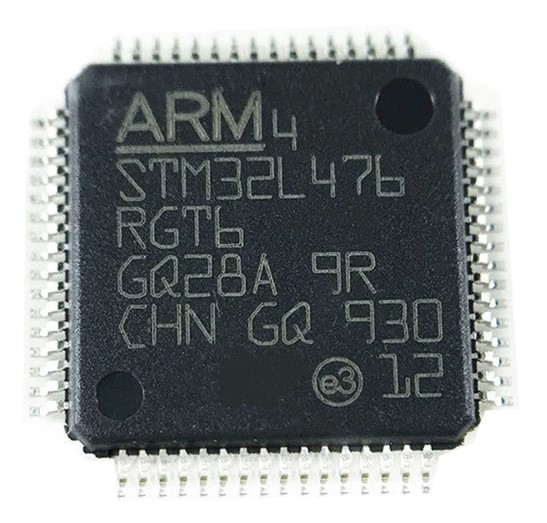
\includegraphics[width=0.7\textwidth]{figures/STM32L476.jpg}
    \end{subfigure}
    \begin{subfigure}{.45\textwidth}
      \centering
      
\includegraphics[width=0.55\textwidth]{figures/LR1110.png}
    \end{subfigure}
    \caption{STM32L476 (left) and LR1110 (right).}
    \label{fig:chips}
\end{figure}

\subsubsection{RF Transceiver}
The \hyperref[bom:lr1110]{LR1110} chip (datasheet: \sbref{app:hardware:lr1110}) is a \ac{LoRa} RF Transceiver with inbuilt Wi-Fi and \ac{GNSS} scanner and is used for geolocation. Wi-Fi includes scanning for 802.11b/g/n Wi-Fi access point \ac{MAC} addresses (\SI{2.4}{\giga\hertz}), while the \ac{GNSS} scanning searches for \ac{GPS}\footnote{GPS: \url{https://www.gps.gov/}}, BeiDou\footnote{BeiDou Navigation Satellite System: \url{http://en.beidou.gov.cn/}}, and geostationary satellite signals. \ac{GNSS} and Wi-Fi scan data is collected on the device and sent to a cloud-based solver to resolve into a position. Semtech provides a Cloud API (fees apply).
cite to LR1110 driver \cite{lr11xx_driver}.

\subsubsection{Temperature Compensated Crystal Oscillator (TCXO)}
A \SI{32}{\mega\hertz} crystal oscillator is the cheapest and lowest power-consuming approach to provide the \SI{32}{\mega\hertz} clock reference to the LR1110 \cite[p.~50]{LR1110_user_manual}.
A \SI{32}{\mega\hertz} \ac{TCXO}\sbref{app:hardware:tcxo} and a \SI{32.768}{\kilo\hertz} clock source are mandatory by the LR1110 for any \ac{GNSS} operation. Further is the \ac{TCXO} a feature to minimise the power consumption required to perform outdoor geolocation \cite[p.~51, p.~132]{LR1110_user_manual}. The heat of the surroundings influences the crystal oscillators, so no copper planes have been added on the \ac{PCB} where crystal oscillators are placed. %Hvad gør forskellen på 1.6V eller 3.3V supply? 

\subsubsection{Accelerometer}
We are implementing an accelerometer to determine if the tracker has been still for a long time or has suddenly moved. We chose \hyperref[bom:lis2de12]{LIS2DE12} (datasheet: \sbref{app:hardware:lis2de12}), an ultra-low-power high-performance 3-axis femto accelerometer. \textit{Femto} meaning that it can detect accelerations on the order of femtometers per second squared (\SI{}{\femto\meter/\second^2}), which is a prefix denoting one quadrillionth ($10^{-15}$) and therefor incredibly small. It has \ac{SPI} and \ac{I2C}, but because \ac{I2C} uses much less power because of the slower speed, we will use that communication protocol - we don't need to send a lot of data back and forth fast.

\begin{figure}[H]
    \centering
    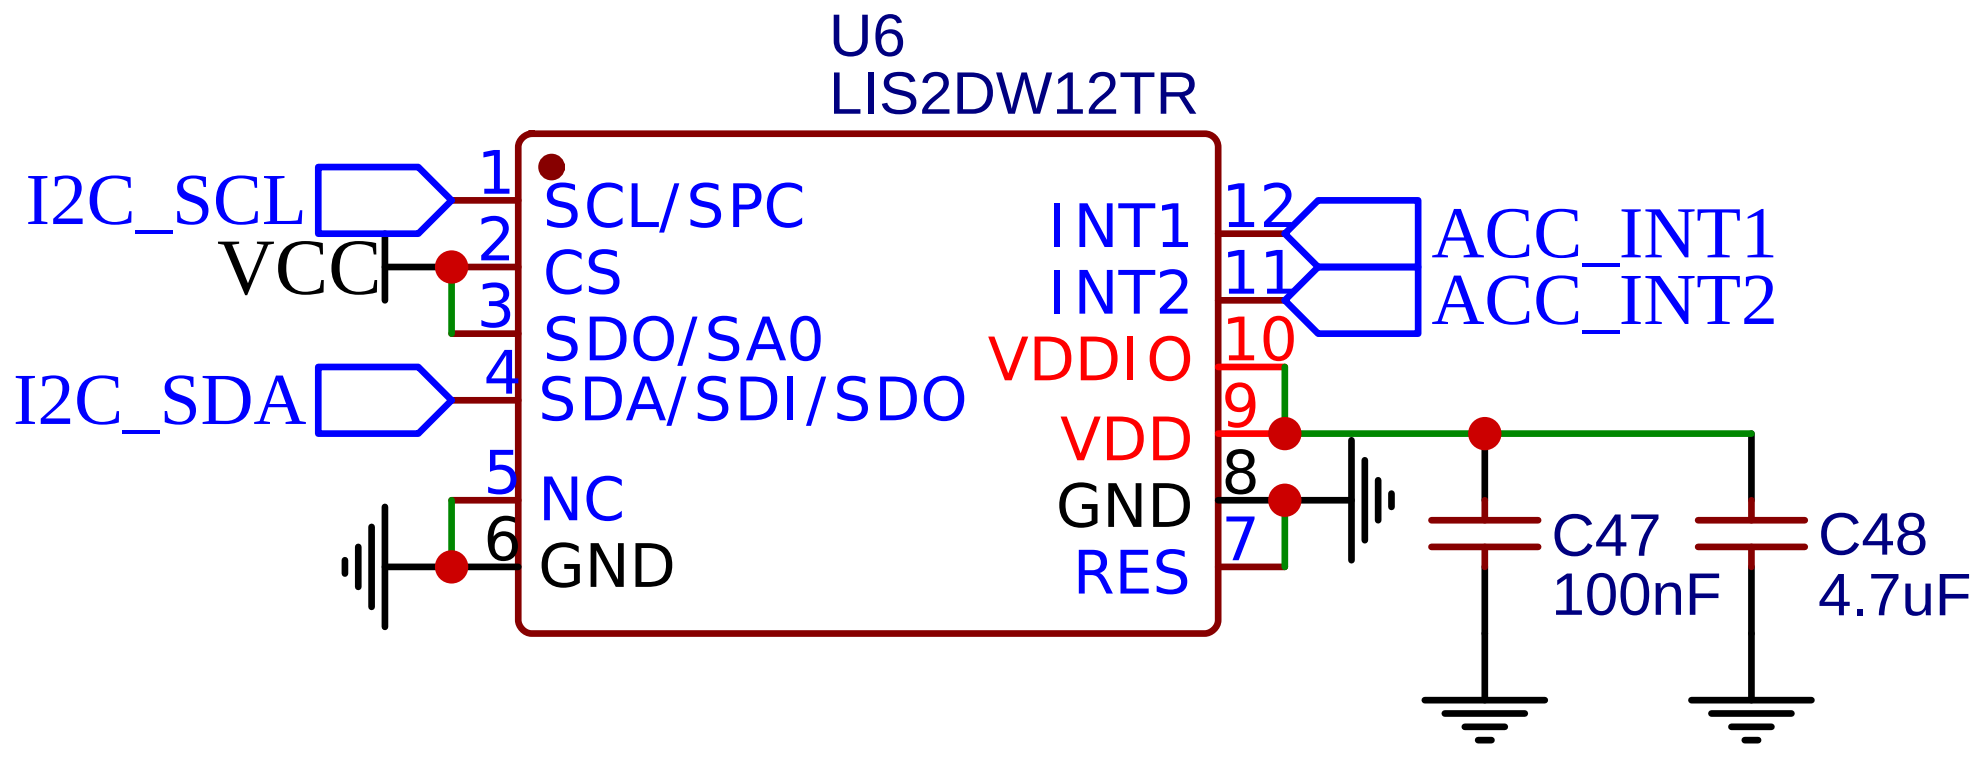
\includegraphics[width=0.6\textwidth]{figures/LIS2DE12.png}
    \caption{Wiring diagram of LIS2DE12.}
    \label{fig:schematic:lis2de12}
\end{figure}

It has two independent programmable interrupt generators for free-fall and motion detection. We will use both (\textit{ACC\_INT1} and \textit{ACC\_INT2}.


table 3.2.1 

Do we need to enable all axes?

It also has click-interrupt which could be used to wake up the tracker or configure it.

\textit{C47} and \textit{C48} are defined from the datasheet \sbref{app:hardware:lis2de12}, p. 19)

\subsubsection{Hall Effect/Magnetic Sensors}
We are implementing a hall effect sensor to make the tracker waterproof and easier to turn on and off. We chose \hyperref[bom:bu52077gwz]{BU52077GWZ-E2} (datasheet: \sbref{app:hardware:BU52077GWZ}). It has a typical operational current of \SI{5}{\micro\ampere} and can operate at a voltage down to \SI{1.65}{\volt}. It has a normal \ac{GPIO} interface and is therefore easy to implement with a simple interrupt on the STM32. This hall effect chip is therefore ideal to work without application.

\begin{figure}[H]
  \centering
  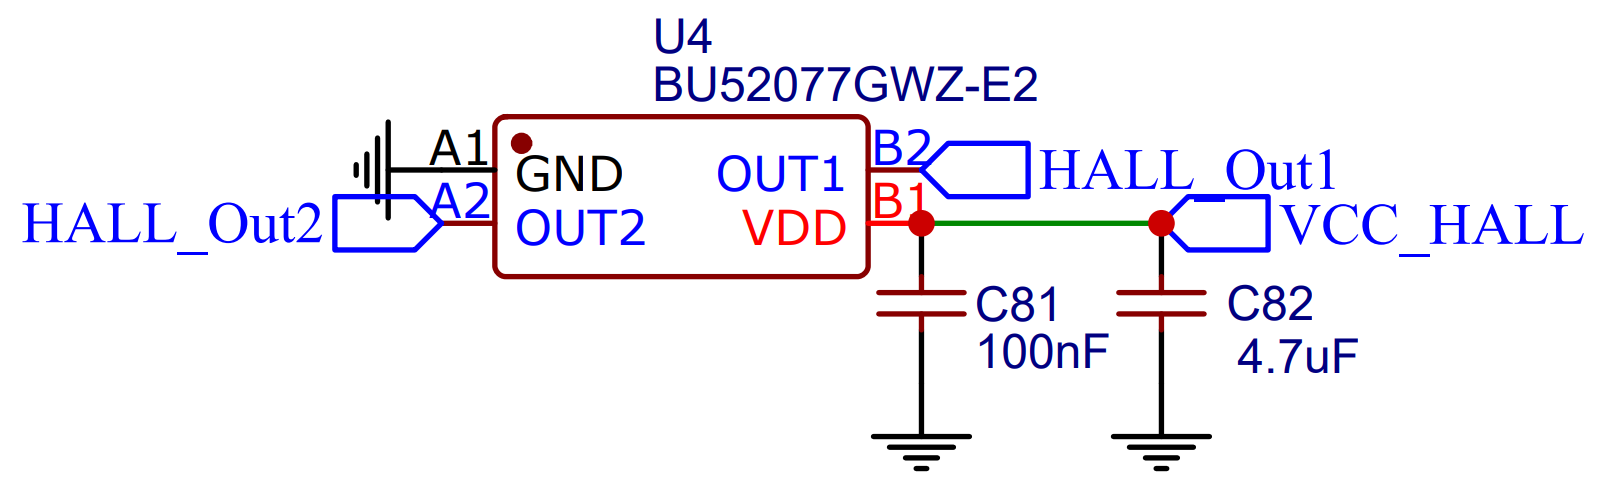
\includegraphics[width=0.6\textwidth]{figures/Hall.PNG}
  \caption{Wiring diagram of BU52077GWZ-E2.}
  \label{fig:schematic:BU52077GWZ}
\end{figure}

\textit{HALL\_OUT1} is triggered when reacting to the south pole of a magnet, and \textit{HALL\_OUT2} is triggered when responding to the magnet's north pole. Therefore, the chip is ideal to switch to turn on and off the tracker.

\subsubsection{GNSS antenna}
Ceramic antenna
We are using a passive \ac{GNSS} antenna which means it has no external electrical components, as all the filtering and powering of the antenna is done directly on the \ac{PCB}.

\hyperref[bom:bga524n6e6327]{BGA 524N6 E6327} (datasheet: \sbref{app:hardware:bga524n6e6327})

\begin{figure}[H]
    \centering
    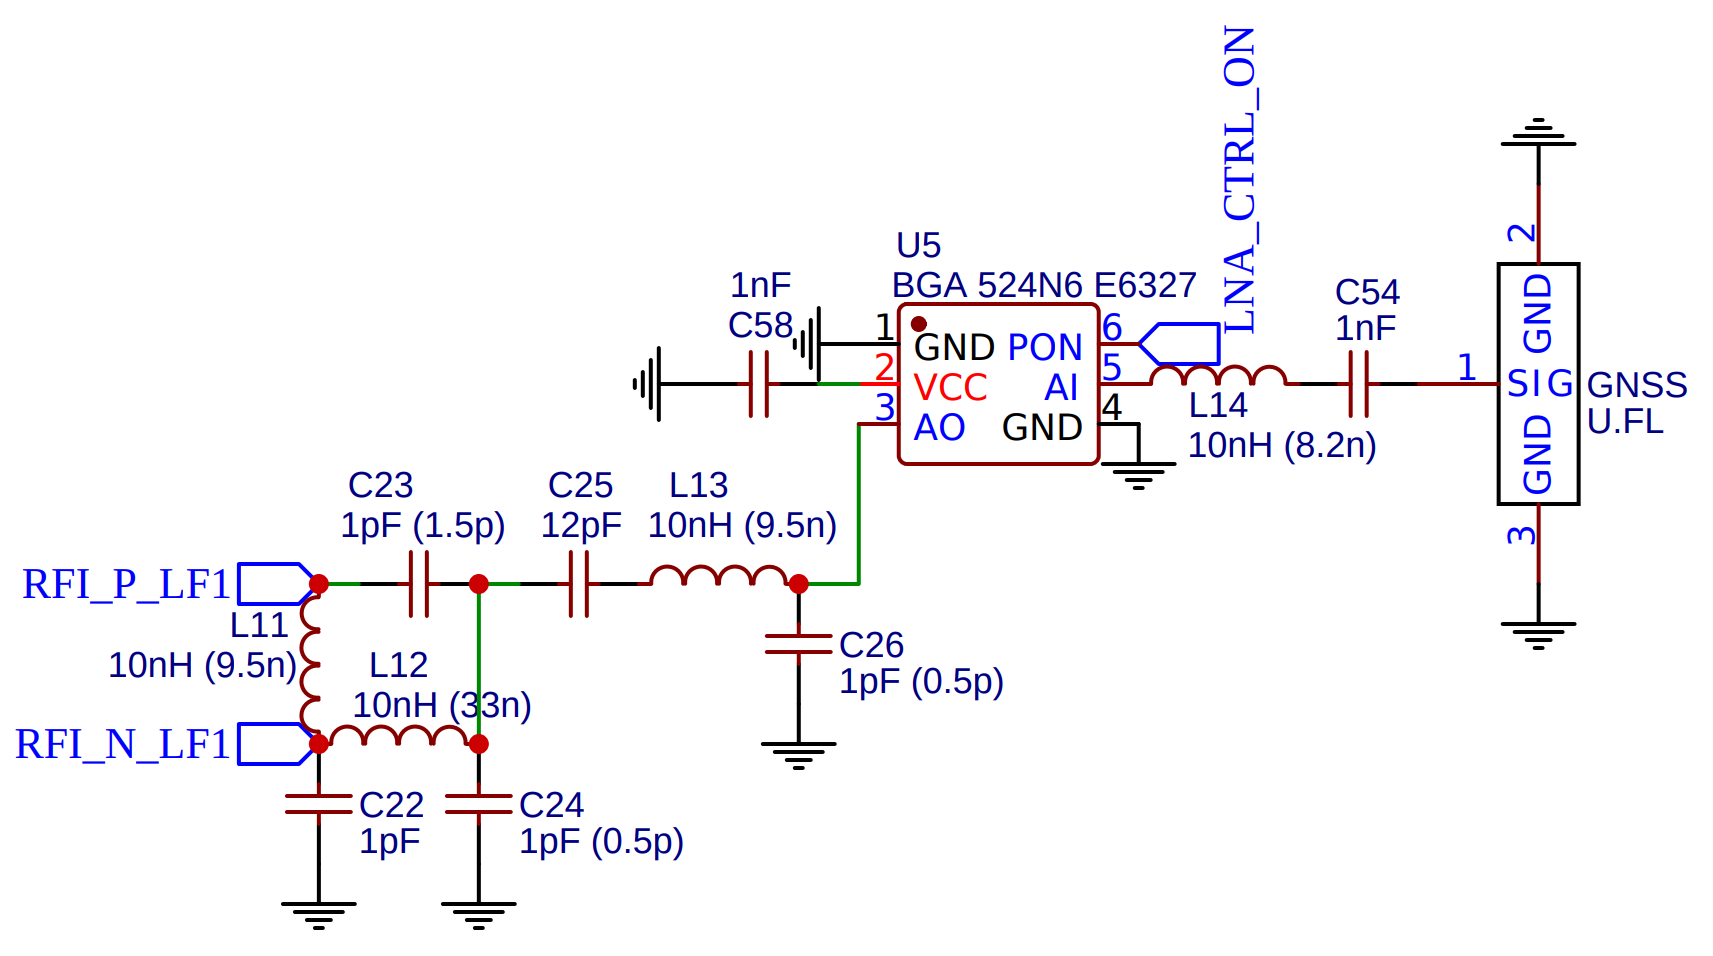
\includegraphics[width=0.9\textwidth]{figures/BGA524N6E6327.png}
    \caption{Wiring diagram of BGA 524N6 E6327.}
    \label{fig:schematic:bga524n6e6327}
\end{figure}

\subsection{Flash and debug a STM32 chip} \label{sec:flash_debug_stm32}
Flashing and debugging any STM32 chip is straightforward. All that is needed is an ST-LINK/V2-1\footnote{\url{https://www.st.com/en/development-tools/st-link-v2.html}} or any STM32 Nucleo board (which already has an ST-LINK/V2-1 built-in). The ST-LINK/V2-1 is connected to the STM32 chip through the \ac{SWD} interface, which is a two-wire interface consisting of a clock (\textit{SWDCLK}) and a data line (\textit{SWDIO}). 

\begin{figure}[H]
  \centering
  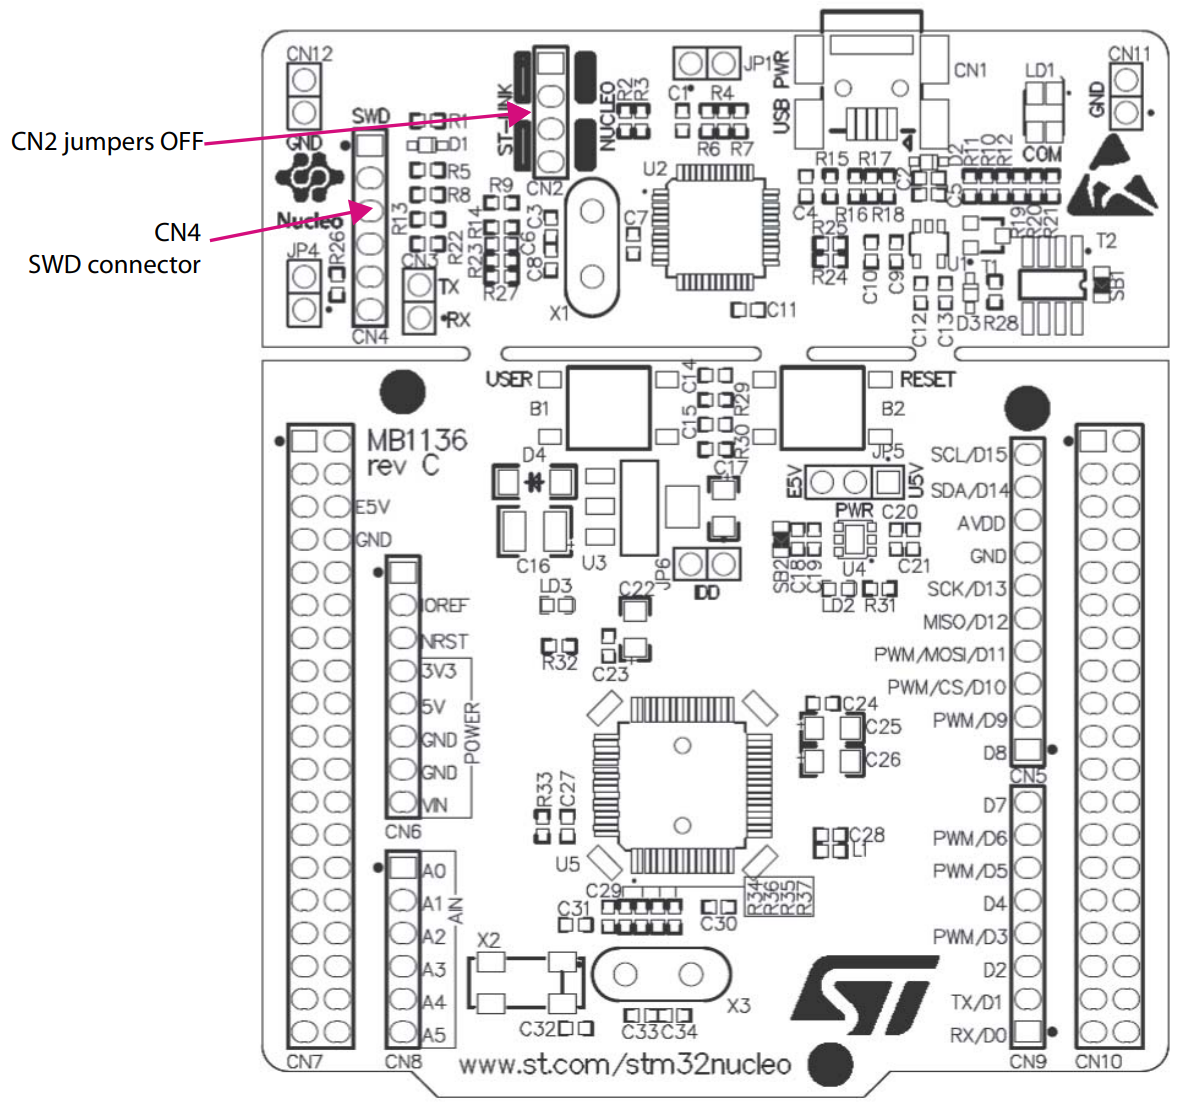
\includegraphics[width=0.7\textwidth]{figures/Nucleo_SWD.png}
  \caption{Using ST-LINK/V2-1 to program the STM32 chip on an external application \cite[p.~19]{STM32_Nucleo_user_manual}.}
  \label{fig:nucleo_swd}
\end{figure}

Per default, the ST-LINK/V2-1 is connected to the in-built STM32-chip on the STM32 Nucleo board. For flashing and debugging the STM32-chip on an external application remove the two jumpers from \textit{CN2} as illustrated in fig.~\ref{fig:nucleo_swd}, and connect the application to the \textit{CN4} debug connector according to fig.~\ref{fig:schematic_stlink}.

\begin{figure}[H]
  \centering
  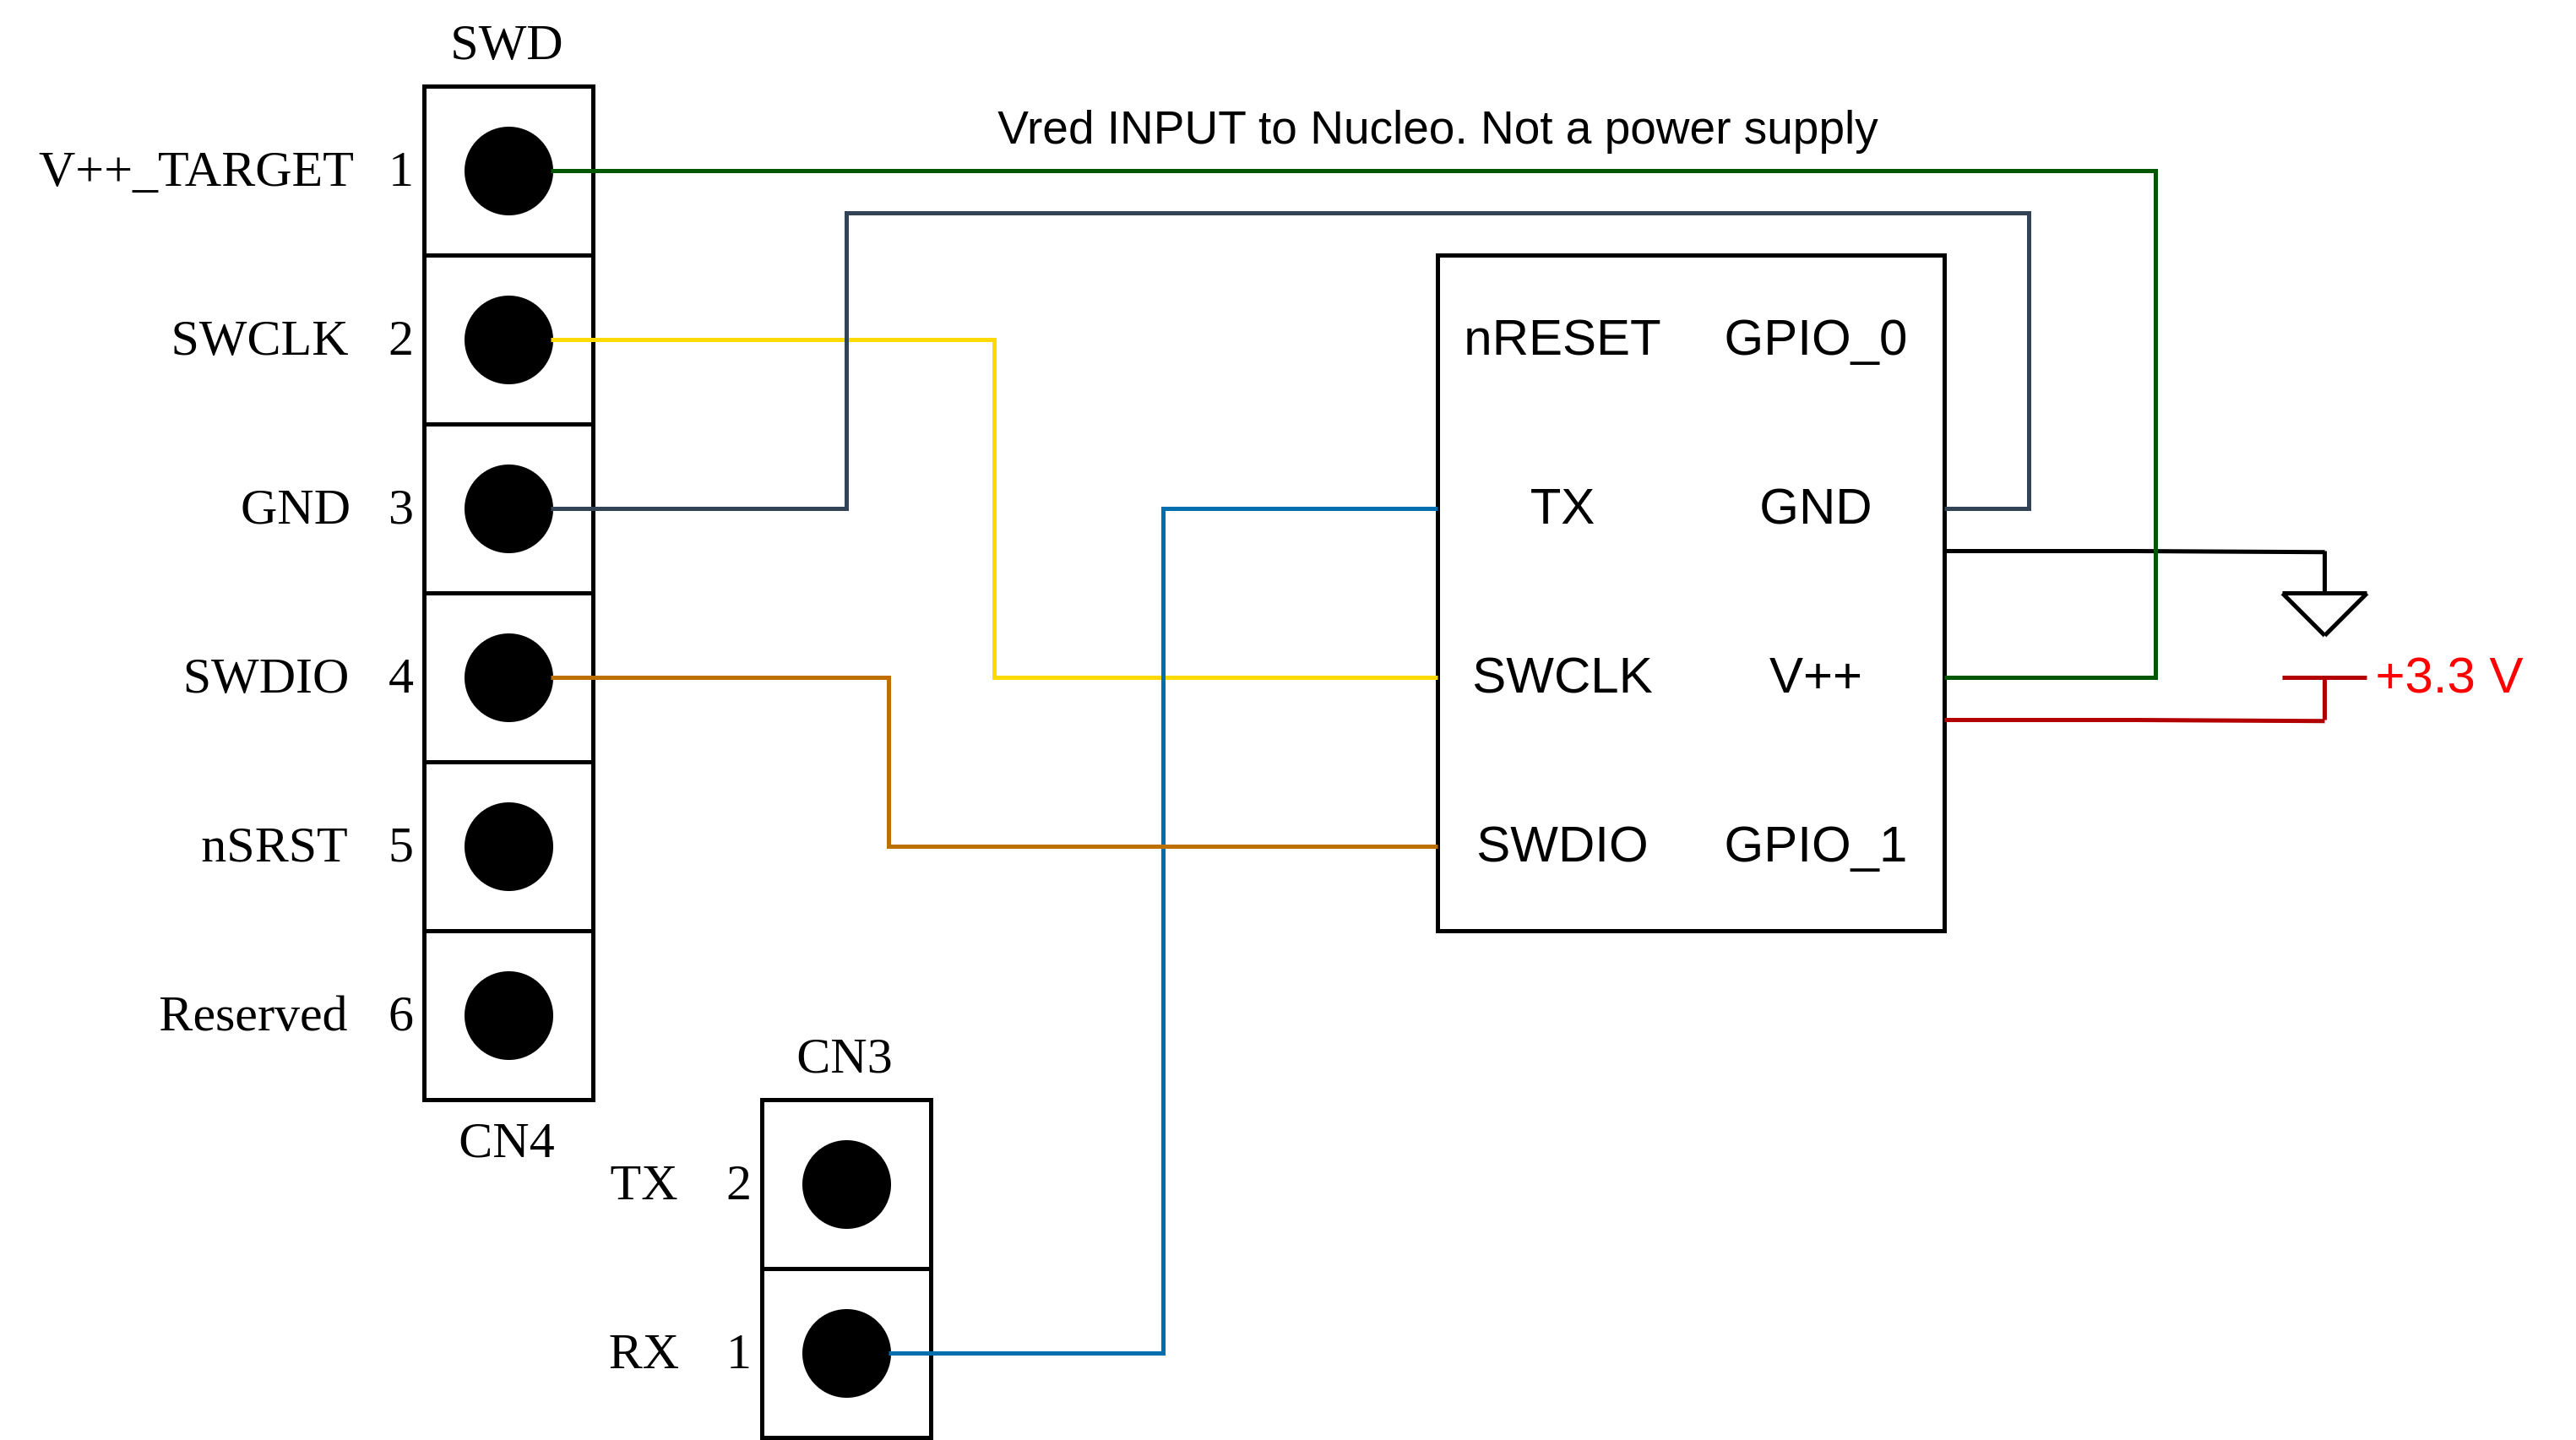
\includegraphics[width=0.8\textwidth]{figures/STLink_SWD_wiring.png}
  \caption{Diagram showing the connection between ST-LINK/V2-1 and a STM32 chip.}
  \label{fig:schematic_stlink}
\end{figure}

For communicating with the STM32-chip over \ac{USART} use the \textit{USART2} interface available on \textit{PA2} and \textit{PA3} of the STM32-chip. To enable the \ac{USART} communication between the ST-LINK/V2-1 and an external application, the related solder bridges \textit{SB13} and \textit{SB14} must be OFF (and \textit{SB62} and \textit{SB63} must be ON if using a Nucleo board and not having cut the board into an ST-LINK part and target STM32 part)\cite[p.~25]{STM32_Nucleo_user_manual}.

The ST-LINK/V2-1 is connected to the computer through \ac{USB}, and the STM32-chip is powered through the ST-LINK/V2-1. The STM32 is flashed with Visual Studio Code or the STM32CubeProgrammer\footnote{\url{https://www.st.com/en/development-tools/stm32cubeprog.html}}, which is a software tool to flash and debug STM32 microcontrollers. Here the STM32 can be debugged, which is done by setting breakpoints in the code and running the code step by step.

\subsection{Choosing transceiver firmware}
It would take up to 6 months longer to implement our own \ac{LoRa} stack

\subsection{Establishing communication with LR1110}
The STM32 and LR1110 communication is through \ac{SPI} (see fig.~\ref{fig:stm32_lr1110_interface}). The LR1110 exposes an \ac{API} which allows the STM32 to communicate with the LR1110 through a set of \ac{SPI} commands and responses.

\begin{figure}[H]
    \centering
    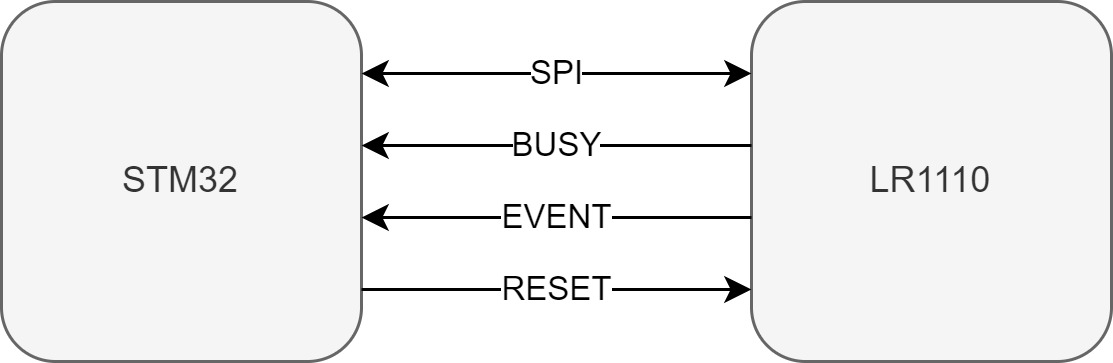
\includegraphics[width=0.6\textwidth]{figures/STM32_LR1110_interface.png}
    \caption{Interface between STM32 and LR1110.}
    \label{fig:stm32_lr1110_interface}
\end{figure}

The \textit{BUSY} signal is used as a handshake to indicate if the LR1110 is ready to accept a command. Therefore, it is necessary to check the status of \textit{BUSY} before sending a command.

The \textit{EVENT} signal is an output signal of the LR1110. This line signals to the STM32 that the device has an asynchronous event data pending. The event can be \ac{LoRaWAN} stack, \ac{GNSS}, or Wi-Fi events. The STM32 must use the \lstinline[style=C++]{GetEventSize(...)} command to determine the event size and \lstinline[style=C++]{GetEvent(...)} command to retrieve such data. The \textit{EVENT} signal stays high until all events are cleared. The STM32 must clear all the events before returning to sleep mode. This prevents the hit from missing the rising edge of the \textit{EVENT} signal when there is a new event. Secondly, this saves several of \SI{}{\micro\ampere} of current consumption when the \textit{EVENT} signal is kept low by the LR1110.

Fig.~\ref{fig:event_example} shows an example of a Wi-Fi passive scan transaction. The STM32 sends a command to the LR1110 to scan for Wi-Fi \ac{AP}s. The LR1110 scans the Wi-Fi \ac{AP}s and stores the data in its internal memory. When the scan is complete, the LR1110 sets the \textit{EVENT} signal high to indicate that there is data to be read. The STM32 then reads the data from the LR1110 with \lstinline[style=C++]{GetEventsize(...)} and \lstinline[style=C++]{GetEvent(...)}, which afterwards then clears the \textit{EVENT} signal.

\begin{figure}[H]
    \centering
    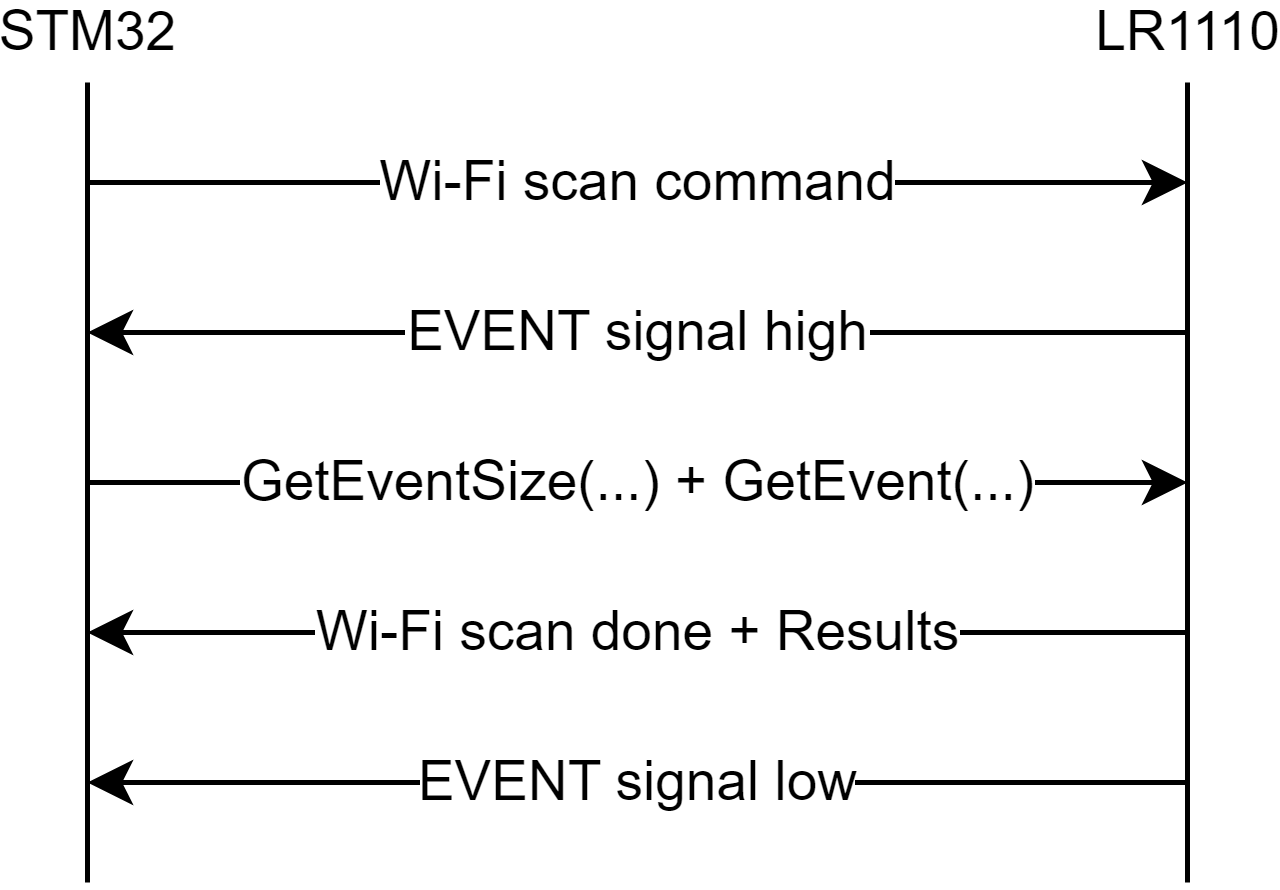
\includegraphics[width=0.5\textwidth]{figures/event_example.png}
    \caption{Example of Wi-Fi passive scan transaction. The transactions are read from top to bottom.}
    \label{fig:event_example}
\end{figure}

Some \ac{SPI} commands generate an immediate response by the LR1110 and therefore do not generate any \textit{EVENT} signal. Such as the command \lstinline[style=C++]{RequestTX(...)} as shown in fig.~\ref{fig:event_example_2}

\begin{figure}[H]
    \centering
    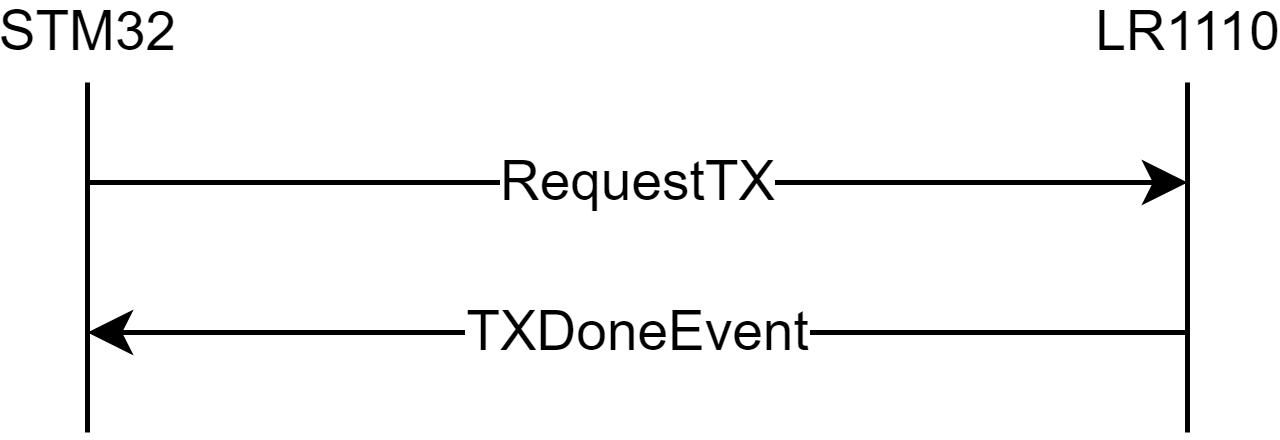
\includegraphics[width=0.5\textwidth]{figures/event_example_2.png}
    \caption{Example of a transaction which does not generate a \textit{EVENT} signal. The transactions are read from top to bottom.}
    \label{fig:event_example_2}
\end{figure}

\subsubsection{Write commands to LR1110}
When executing write commands (see fig.~\ref{fig:write_command}), the LR1110 transmits status registers and interrupt registers to the STM32 through the \textit{MOSI} pin, contingent upon the command opcode and its accompanying arguments. The host initiates by sending a 16-bit opcode (\textit{Op0} and \textit{Op1}), followed by the necessary arguments (\textit{Arg0}, \textit{Arg1}, etc.). Activation of the \textit{BUSY} signal occurs automatically upon the falling edge of the \textit{NSS}. Subsequently, once the LR1110 completes processing the command, the \textit{BUSY} signal is disengaged, signalling readiness to accept another command.

\iffalse
%wavedrom
{signal: [
  {name: 'BUSY', wave: '0.1.......................|0'},
  {name: 'NSS', wave: '10.......................1|.'},
  {name: 'MOSI', wave: 'x..5..5..7..7..7..7..7..xxxx', data: ['Op0', 'Op1', 'Arg0', 'Arg1', 'Arg2', 'Arg3', 'Arg4']},
  {name: 'MISO', wave: 'x..3..3..4..4..4..4..2..xxxx', data: ['Stat1', 'Stat2', 'IrqStat(31:24)', 'IrqStat(23:16)', 'IrqStat(15:8)', 'IrqStat(7:0)', '0']},
]}
\fi
\begin{figure}[H]
    \centering
    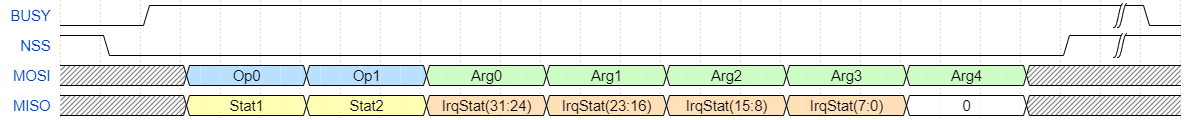
\includegraphics[width=1\textwidth]{figures/write_command.png}
    \caption{Write SPI command timing diagram.}
    \label{fig:write_command}
\end{figure}

\subsubsection{Read commands from LR1110}
Specific read commands extract LR1110 data, encompassing internal status or geolocation outcomes (fig.~\ref{fig:read_command} shows an example of reading data from the LR1110). The STM32 initiates by dispatching a 16-bit opcode (\textit{Op0} and \textit{Op1}), supplemented by arguments as necessary (\textit{Arg0}, \textit{Arg1}, etc.). Activation of the \textit{BUSY} signal occurs automatically upon the falling edge of the \textit{NSS}. Upon completion of data preparation by the LR1110, the \textit{BUSY} signal is disengaged. Subsequently, the host can retrieve the data by transmitting NOPs (\texttt{0x00} bytes) to sequentially extract the data via the \ac{SPI}.

\iffalse
%wavedrom
{signal: [
  {name: 'BUSY', wave: '0.1..............|0.1...........0'},
  {name: 'NSS', wave: '10..............1|.0...........1.'},
  {name: 'MOSI', wave: 'x..5..5..7..7..xxxxxx8..8..8..xxx', data: ['Op0', 'Op1', 'Arg0', 'Arg1', 'NOP', 'NOP', 'NOP']},
  {name: 'MISO', wave: 'x..3..3..4..4..xxxxxx3..6..6..xxx', data: ['Stat1', 'Stat2', 'IrqStat(31:24)', 'IrqStat(23:16)', 'Stat1', 'Rsp0', 'Rsp1']},
]}
\fi
\begin{figure}[H]
    \centering
    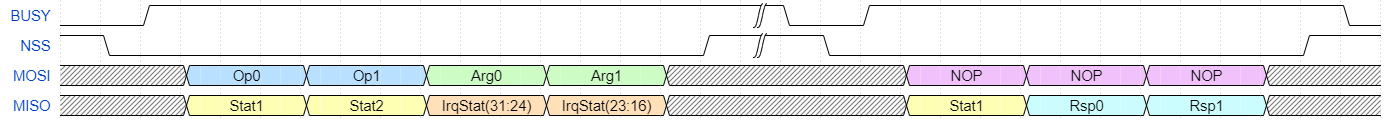
\includegraphics[width=1\textwidth]{figures/read_command.png}
    \caption{Read SPI command timing diagram.}
    \label{fig:read_command}
\end{figure}

One thing to notice is that when writing commands to LR1110 is that \textit{Stat1} and \textit{Stat2} refer to the former write command, not the current command that has just been sent. However, does \textit{Stat1} (from the read command) refer to the status for the current command.

\subsection{Implementation of tracking features}
In the following sections, we will describe how we implement geolocation. We will report on how we have implemented Wi-Fi scanning, satellite scanning, \ac{LoRa}-communication, and other notable features. We will also describe how we have implemented the power-saving features.

\subsubsection{Wi-Fi scanning}
Scanning of Wi-Fi \ac{AP}s is done by setting the channels and the time to scan each channel. The LR1110 will scan the Wi-Fi \ac{AP}'s and store the data in the internal memory. The STM32 chip can then read the data.

\subsubsection{Satellite scanning}
The LR1110 can scan for \ac{GPS}, BeiDou, and geostationary satellites. The scanning is done by setting the time to scan and then starting the scan. The STM32 chip can then read the data.

\subsection{Power minimising}
One of the other big sections in the report, as the title is ultra-low power. Here we will describe how we have tried to minimise power consumption.

What is ultra-low power and what is low power?

Maybe it won't be easy to write since it is probably an iterative process. We test which methods work best, and then change something until we have found the best method.


For a stable power supply, we are using the \ac{LDO} Voltage Regulators \hyperref[bom:xc6220]{XC6220B331MR} (datasheet: \sbref{app:hardware:XC6220}). The chip is a \SI{3.3}{\volt} voltage regulator with a input voltage ranging from \SI{1.6}{\volt} to \SI{6.0}{\volt} and a maximum output current of \SI{1000}{\milli\ampere}. The quiescent current is \SI{8}{\micro\ampere} and the dropout voltage is around \SI{20}{\milli\volt}. A voltage regulator is crucial for any battery-powered device. It has high power- and low power mode, which means the quiescent current and dropout voltage can be reduced if the device is in low power mode. When the output current is less than \SI{1}{\milli\ampere} (minimum), the quiescent current is reduced to \SI{8}{\micro\ampere}. If the output current becomes \SI{10}{\milli\ampere} (maximum) or more, the mode changes automaticcaly to the high power mode and the chip returns to high speed operation.

\subsection{PCB Design}
We are using EasyEDA\footnote{\url{https://easyeda.com/}} to design the \ac{PCB} and JLCPCB\footnote{\url{https://jlcpcb.com/}} to manufacture them.

\subsubsection{Impedance}
For determining the impedance and maintaining this throughout the \ac{PCB}, the layout of the components and stackup of the \ac{PCB} is important. We chose a 4-layer \ac{PCB} as this is preferable to optimise \ac{RF} \ac{PCB} layout, especially if there is dense routing. 

Any \ac{RF} line can potentially radiate or receive interfering signals, which is why the \ac{RF} trace between the antenna and the matching network is designed using a \ac{GCPW} structure as shown fig.~\ref{fig:gcpw}. This means that the second layer is one full layer for a clean ground plane below the \ac{RF} to minimize \ac{EMC} problems. The \ac{GCPW} is dimensioned to have a characteristic impedance equal to the antenna impedance, which we chose to be \SI{50}{\ohm}.

\begin{figure}[H]
    \centering
    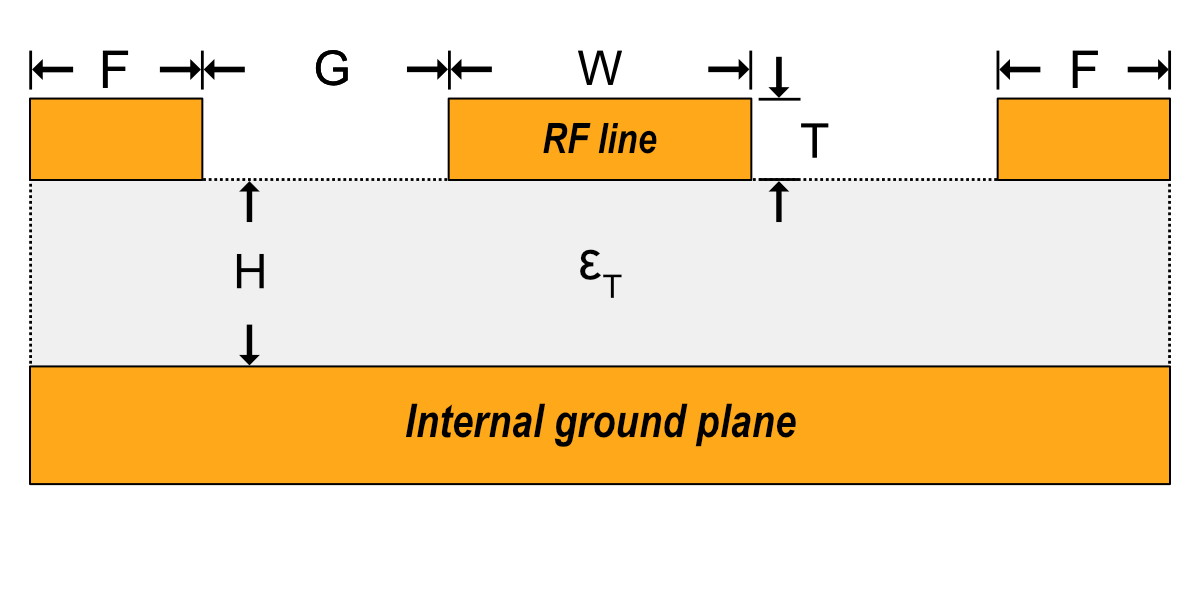
\includegraphics[width=0.6\textwidth]{figures/GCPW.png}
    \caption{Cross section of RF line layout. Here, the layer closest to the RF line is a ground layer, which will minimize any EMC issues.}
    \label{fig:gcpw}
\end{figure}

Choosing JCLPSB's JLC04101H-7628 Stackup has a dielectric constant of $\kappa = 4.4$ which will suit this project. The stackup is described in tab.~\ref{tab:pcb_stackup}.

\begin{table}[H]
    \centering
    \caption{Stackup of JLC04101H-7628 with PCB thickness of \SI{1.0}{\milli\meter}, outer copper weight of \SI{0.4}{\ounce}, and inner copper weight of \SI{0.5}{\ounce}\protect\footnotemark.}
    \label{tab:pcb_stackup}
    \begin{tabular}{lll}
    \textbf{Layer} & \textbf{Material Type} & \textbf{Thickness} \\ \hline
    Top Layer & \cellcolor{copper_green}Copper & \SI{0.035}{\milli\meter} \\
    Prepreg & 7628 & \SI{0.2104}{\milli\meter} \\
    Internal Ground Plane & \cellcolor{copper_green}Copper & \SI{0.0152}{\milli\meter} \\
    Core & \cellcolor{core_yellow}Core & \SI{0.45}{\milli\meter} \\
    Internal Power Plane & \cellcolor{copper_green}Copper & \SI{0.0152}{\milli\meter} \\
    Prepreg & 7628 & \SI{0.2104}{\milli\meter} \\
    Bottom Layer & \cellcolor{copper_green}Copper & \SI{0.035}{\milli\meter}
    \end{tabular}
\end{table}
\footnotetext{\url{https://jlcpcb.com/impedance}}

To calculate the transmission line characteristic impedance [$\Omega$] we will use Coplanar Waveguide by AppCAD \sbref{app:software:appcad}. Fig.~\ref{fig:appcad} shows the top layer, prepreg, and the internal ground plane.

\begin{figure}[H]
    \centering
    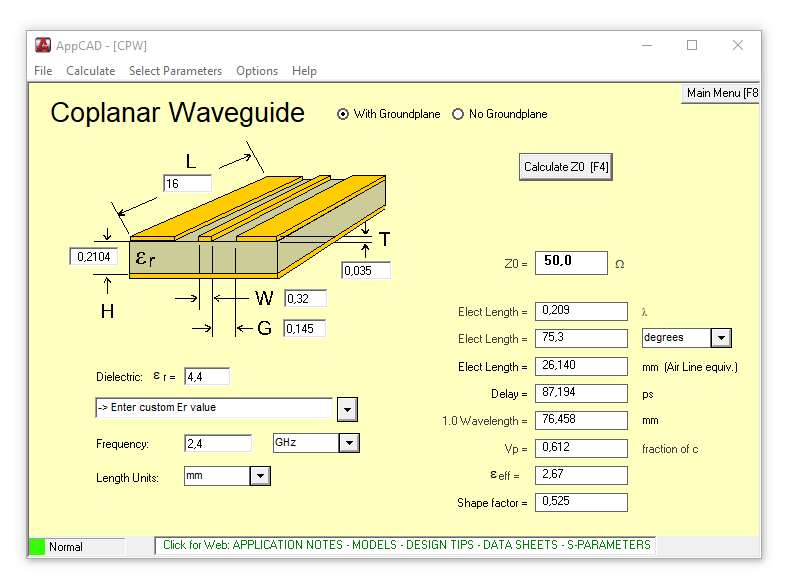
\includegraphics[width=1.0\textwidth]{figures/appcad_16.PNG}
    \caption{AppCAD Coplanar Waveguide: Calculating the impedance of the Wi-Fi RF line.}
    \label{fig:appcad}
\end{figure}

According to the PCB Design Guideline for LR1110, shall \textit{G}, \textit{W}, \textit{T}, \textit{H}, and $\epsilon_r$ (see diagram in fig.~\ref{fig:appcad}) be determined to ensure \SI{50}{\ohm} with coplanar waveguide with ground to \ac{RF} line. \textit{W} must be constant all along the \ac{RF} path, and if possible the same width as the components' pads. Furthermore, must the vias be stitches at a distance of a least $D = \lambda / 20 = \SI{52.915}{\milli\meter} / 20 = \SI{2.645}{\milli\meter}$ \cite[p.~9-11]{LR1110_pcb_design_guide}. The width of the ground on each side of the \ac{RF} line \textit{F} (see fig.~\ref{fig:gcpw}) must be larger than the width of the \ac{RF} line \textit{W} + the gap \textit{G}; $F > W + G$. Even if two \ac{RF} lines are close to each other (e.g. the \ac{RF} lines for \ac{LoRa}), then some ground should separate them to avoid coupling \cite[p.~20-21]{LR1110_pcb_design_guide}.

Most components on the \ac{RF} line have a width of around \SI{0.5}{\milli\meter}, which is why we chose \textit{W} to be \SI{0.5}{\milli\meter}. We chose the thickness of the \ac{PCB} to be \SI{1}{\milli\meter} and according to JLC04101H-7628 does \textit{T} have the height of \SI{0.035}{\milli\meter} and H would then be \SI{0.2104}{\milli\meter}. We would then choose \textit{G} to be \SI{0.5}{\milli\meter} so we are achieving an impedance of the RF line to be \SI{50}{\ohm}.

From this, we chose the \ac{PCB} design rules to be:
Track width: \SI{0.254}{\milli\meter} \\
Clearance: \SI{0.145}{\milli\meter} \\
Via diameter: \SI{0.25}{\milli\meter} \\
Via drill diameter: \SI{0.15}{\milli\meter}

\subsubsection{PCB design versions}
Our first version (fig.~\ref{fig:pcb_v1}) of the \ac{PCB} was designed to experiment with debugging and flashing the STM32-chip. It was a simple 2-layer \ac{PCB} with few components and oscillators for basic operations. We added \ac{LED}'s, \ac{USART} for debugging, and the footprint for the LR1110 chip, which we could test if we managed to flash and debug the STM32 chip. The LR1110 chip was added as a hat/shield to remove it better if something was not working immediately. After following instructions from sec.~\ref{sec:flash_debug_stm32} we quickly were able to flash the chip and later debug.

\begin{figure}[H]
    \centering
    \begin{minipage}[c]{0.49\textwidth}
        \centering
        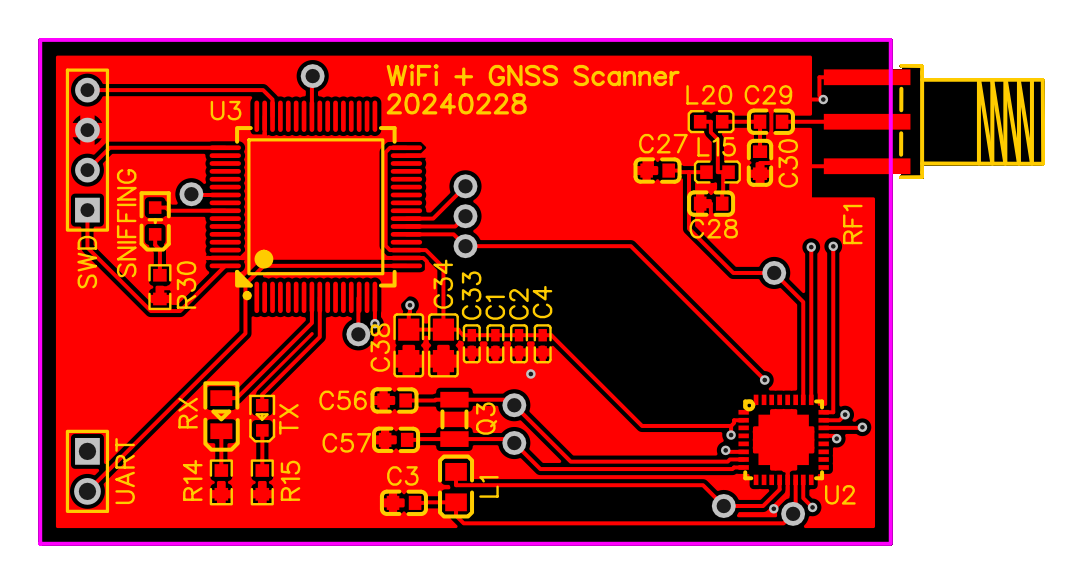
\includegraphics[width=\textwidth]{figures/PCB_v1.png}
    \end{minipage}
    \hfill
    \begin{minipage}[c]{0.49\textwidth}
        \centering
        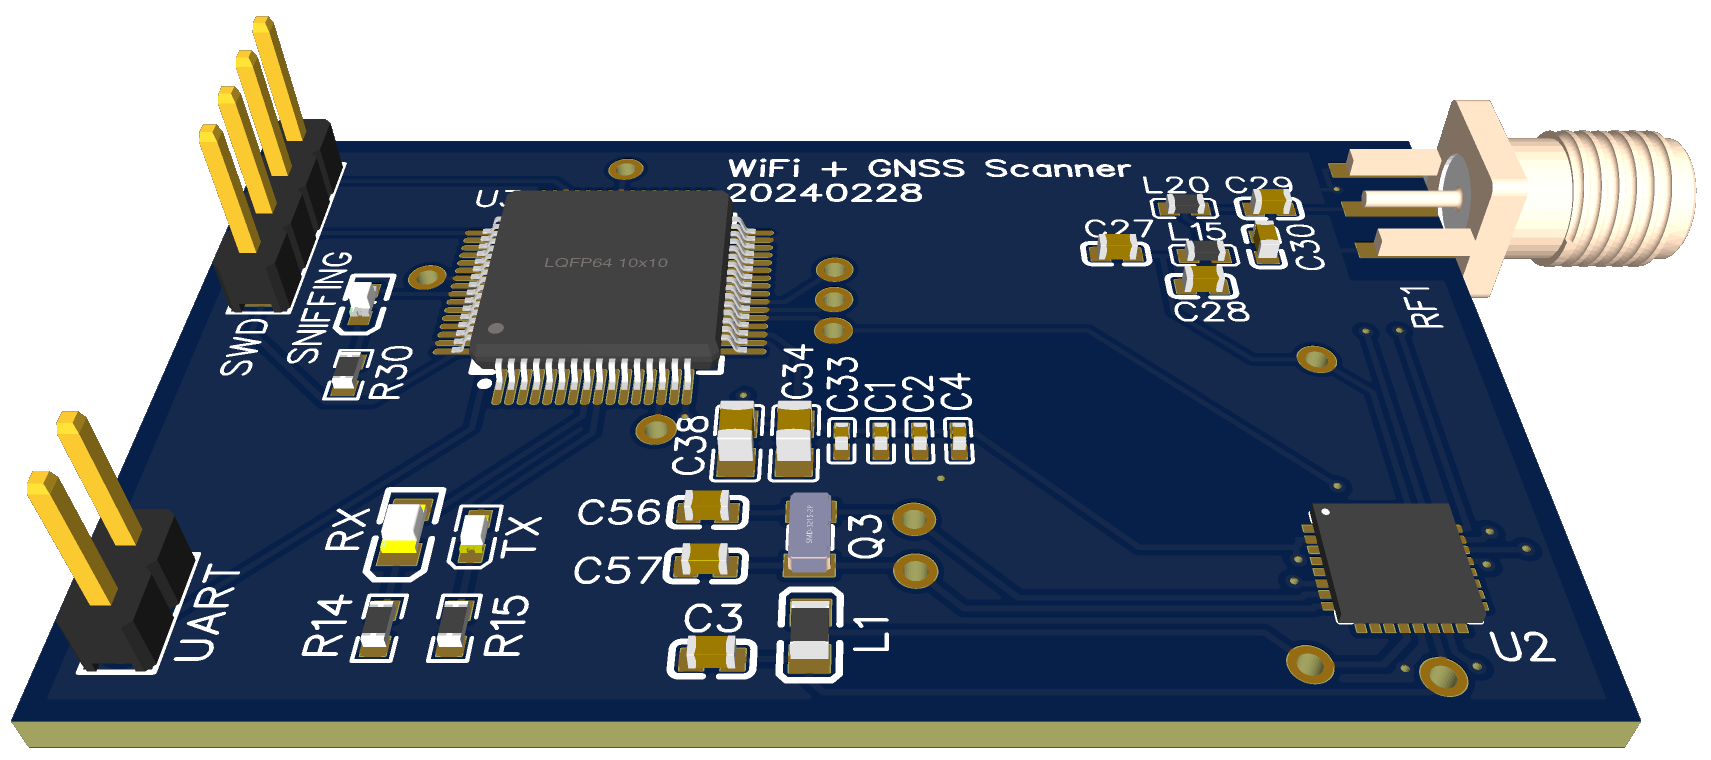
\includegraphics[width=\textwidth]{figures/PCB_v1_3D.png}
    \end{minipage}
    \caption{\nth{1} version of our PCB. \si{32} $\times$ \SI{54}{\milli\meter}.}
    \label{fig:pcb_v1}
\end{figure}

After the success of being able to fast flash and debug the system, we designed the second version (fig.~\ref{fig:pcb_v2}). This time, we designed a 4-layer \ac{PCB} for better routing and having a whole plane just for the ground. We added the \ac{RF}-lines for Wi-Fi, \ac{GNSS} and \ac{LoRa}. Furthermore, did we add a \SI{3.3}{\volt} voltage regulator, a reset switch, and the accelerometer to determine if the tracker has been moving.

\begin{figure}[H]
    \centering
    \begin{minipage}[c]{0.49\textwidth}
        \centering
        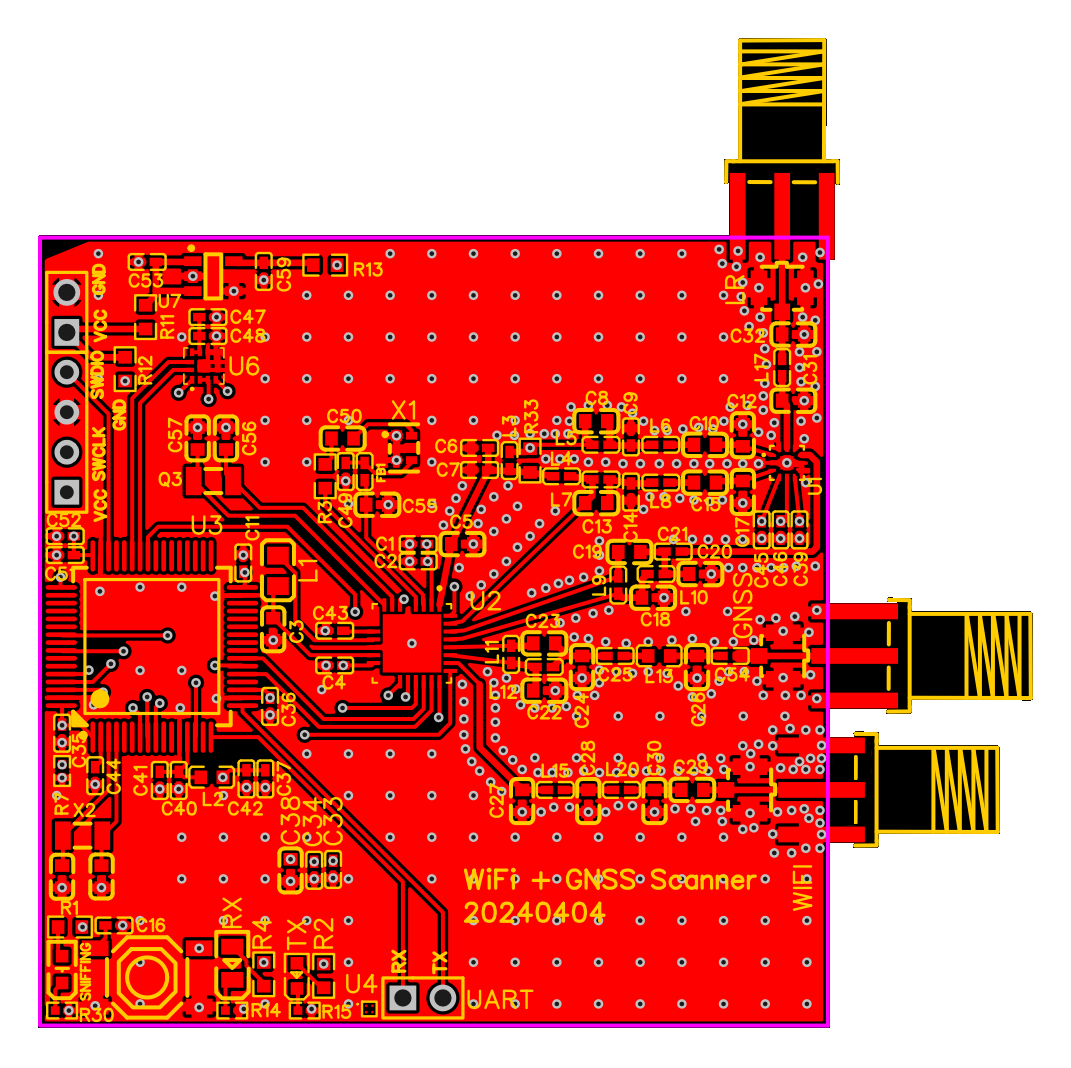
\includegraphics[width=\textwidth]{figures/PCB_v2.png}
    \end{minipage}
    \hfill
    \begin{minipage}[c]{0.49\textwidth}
        \centering
        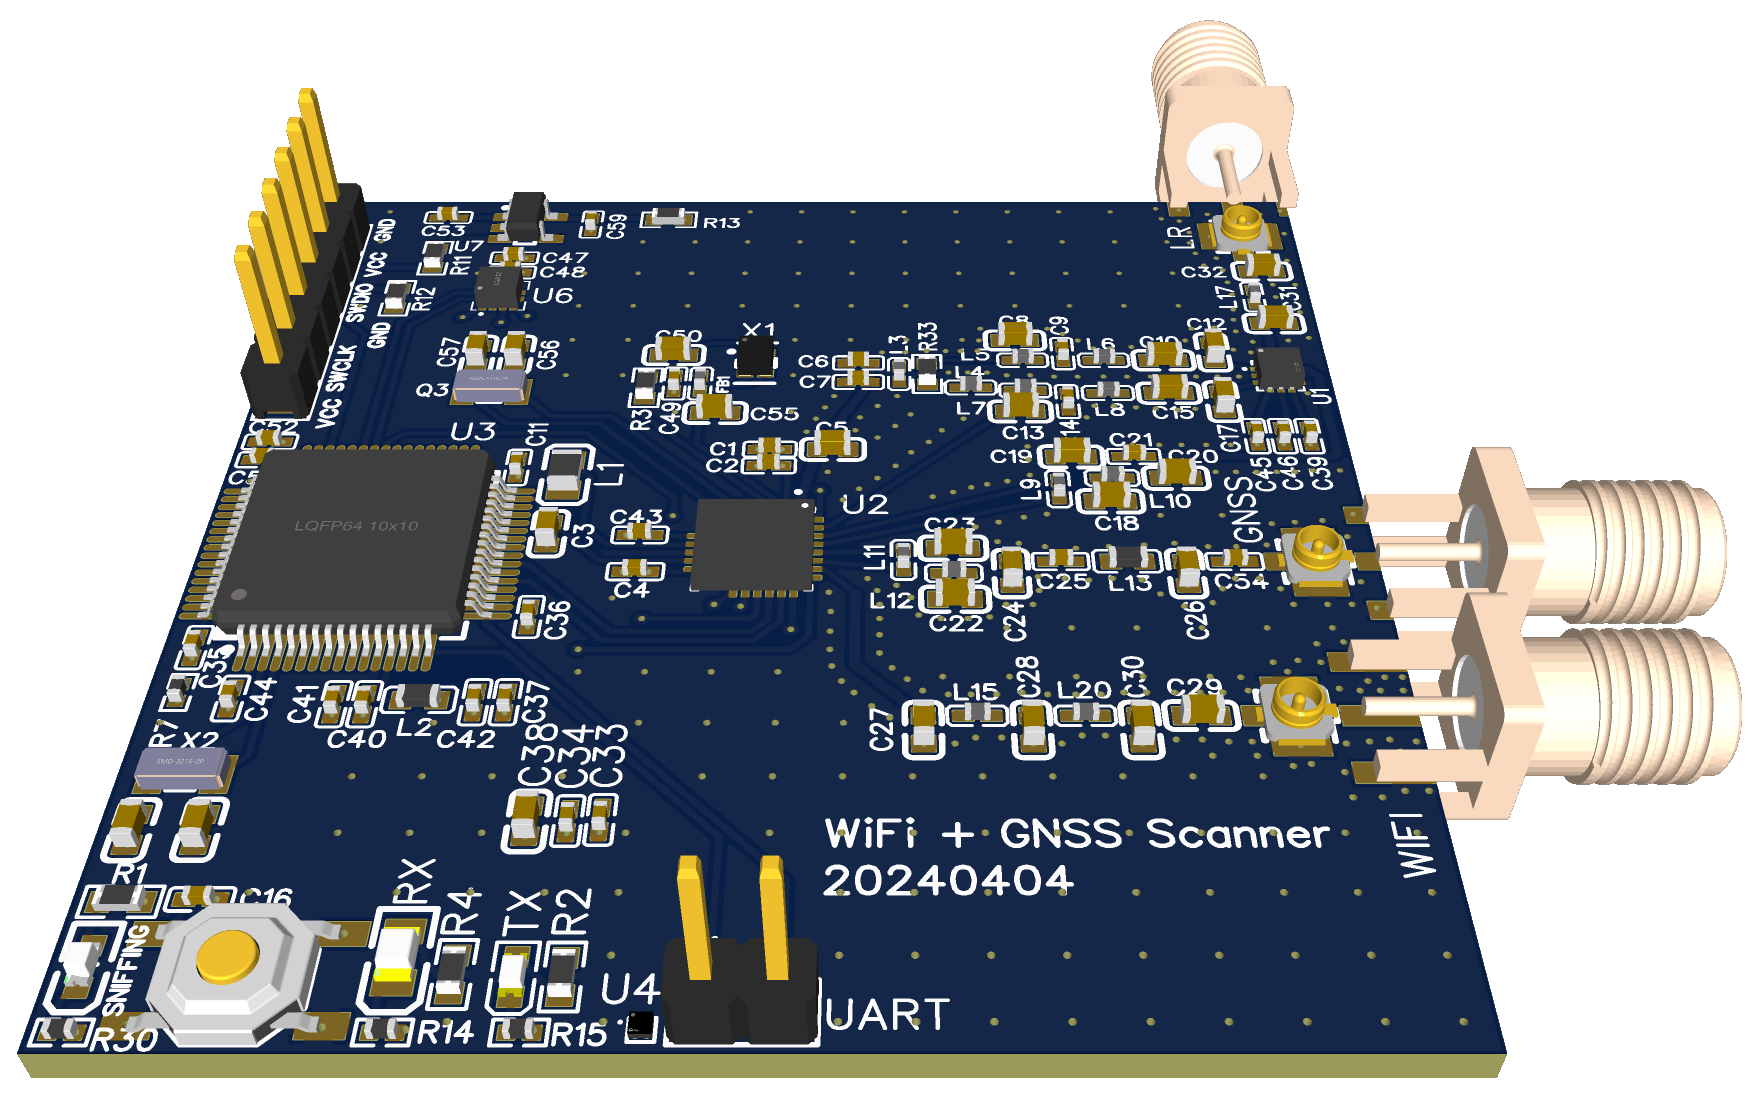
\includegraphics[width=\textwidth]{figures/PCB_v2_3D.png}
    \end{minipage}
    \caption{\nth{2} version of our PCB. \si{50} $\times$ \SI{50}{\milli\meter}.}
    \label{fig:pcb_v2}
\end{figure}

For the \nth{3} and final version of our \ac{PCB} (fig.~\ref{fig:pcb_v3}), we removed the \ac{LED}s and the reset button to make the board smaller (the pins were still there, which means that with the combination of a hat/shield still could be used). The size of the final \ac{PCB} is \si{33} $\times$ \SI{49}{\milli\meter}. We added the hall effect sensor and removed the big SMA antenna connectors instead of the smaller U.FL connectors.

\begin{figure}[H]
    \centering
    \begin{minipage}[c]{0.49\textwidth}
        \centering
        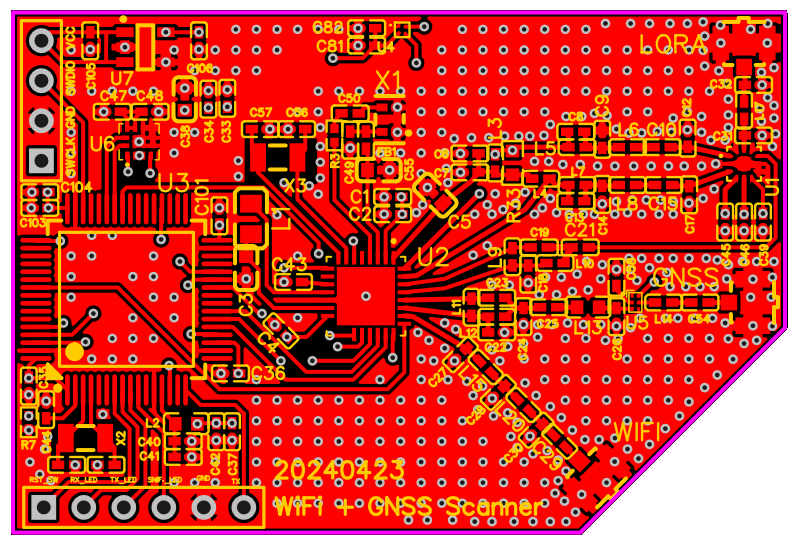
\includegraphics[width=\textwidth]{figures/PCB_v3.png}
    \end{minipage}
    \hfill
    \begin{minipage}[c]{0.49\textwidth}
        \centering
        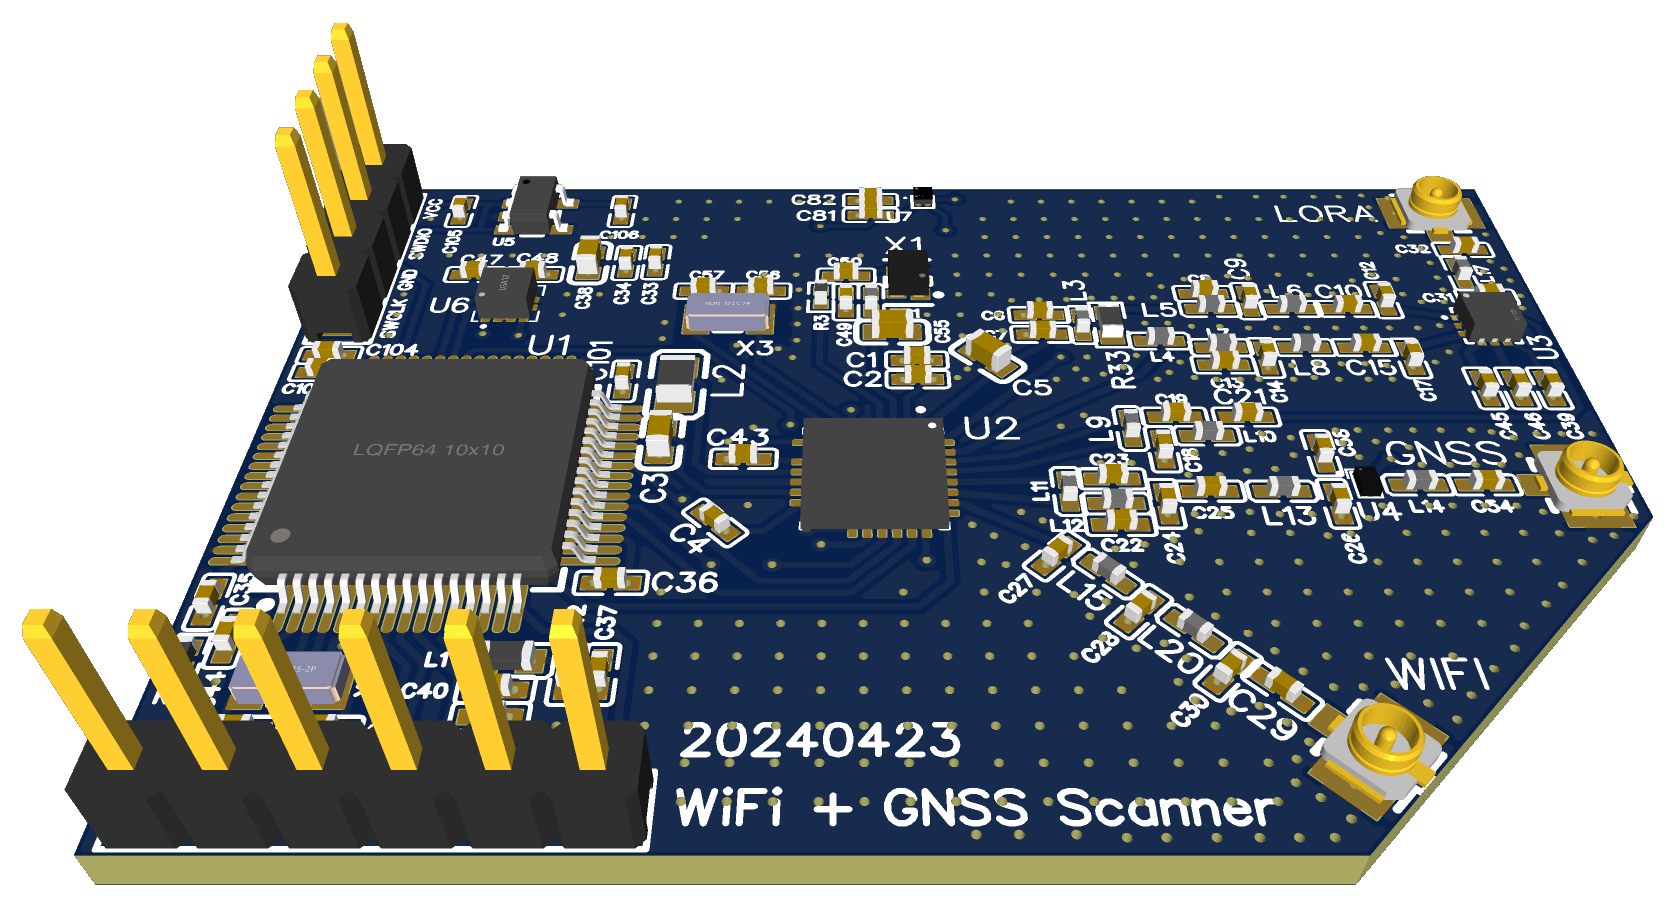
\includegraphics[width=\textwidth]{figures/PCB_v3_3D.png}
    \end{minipage}
    \caption{\nth{3} version of our PCB. \si{33} $\times$ \SI{49}{\milli\meter}. A larger version can be found in app.~\ref{app:PCB} and app.~\ref{app:3DView}}
    \label{fig:pcb_v3}
\end{figure}

As most of the components are tiny and sometimes will shorten when soldering on, X-ray images (see fig.~\ref{fig:x_ray}) need to be taken to verify no shorting of the components.

\begin{figure}[H]
    \centering
    
\includegraphics[width=0.5\textwidth]{figures/x_ray.jpg}
    \caption{X-ray (\SI{90}{\kilo\volt}, \SI{80}{\micro\volt}) image of the smallest components. The component (U4: \hyperref[bom:bga524n6e6327]{BGA524N6E6327}) with the 6 pins has a size of $1.1$ × \SI{0.7}{\milli\meter}.}
    \label{fig:x_ray}
\end{figure}

\subsubsection{Wiring diagram}
Fig.~\ref{fig:schematic} shows the wiring schematic of the tracker.

\begin{figure}[H]
    \centering
    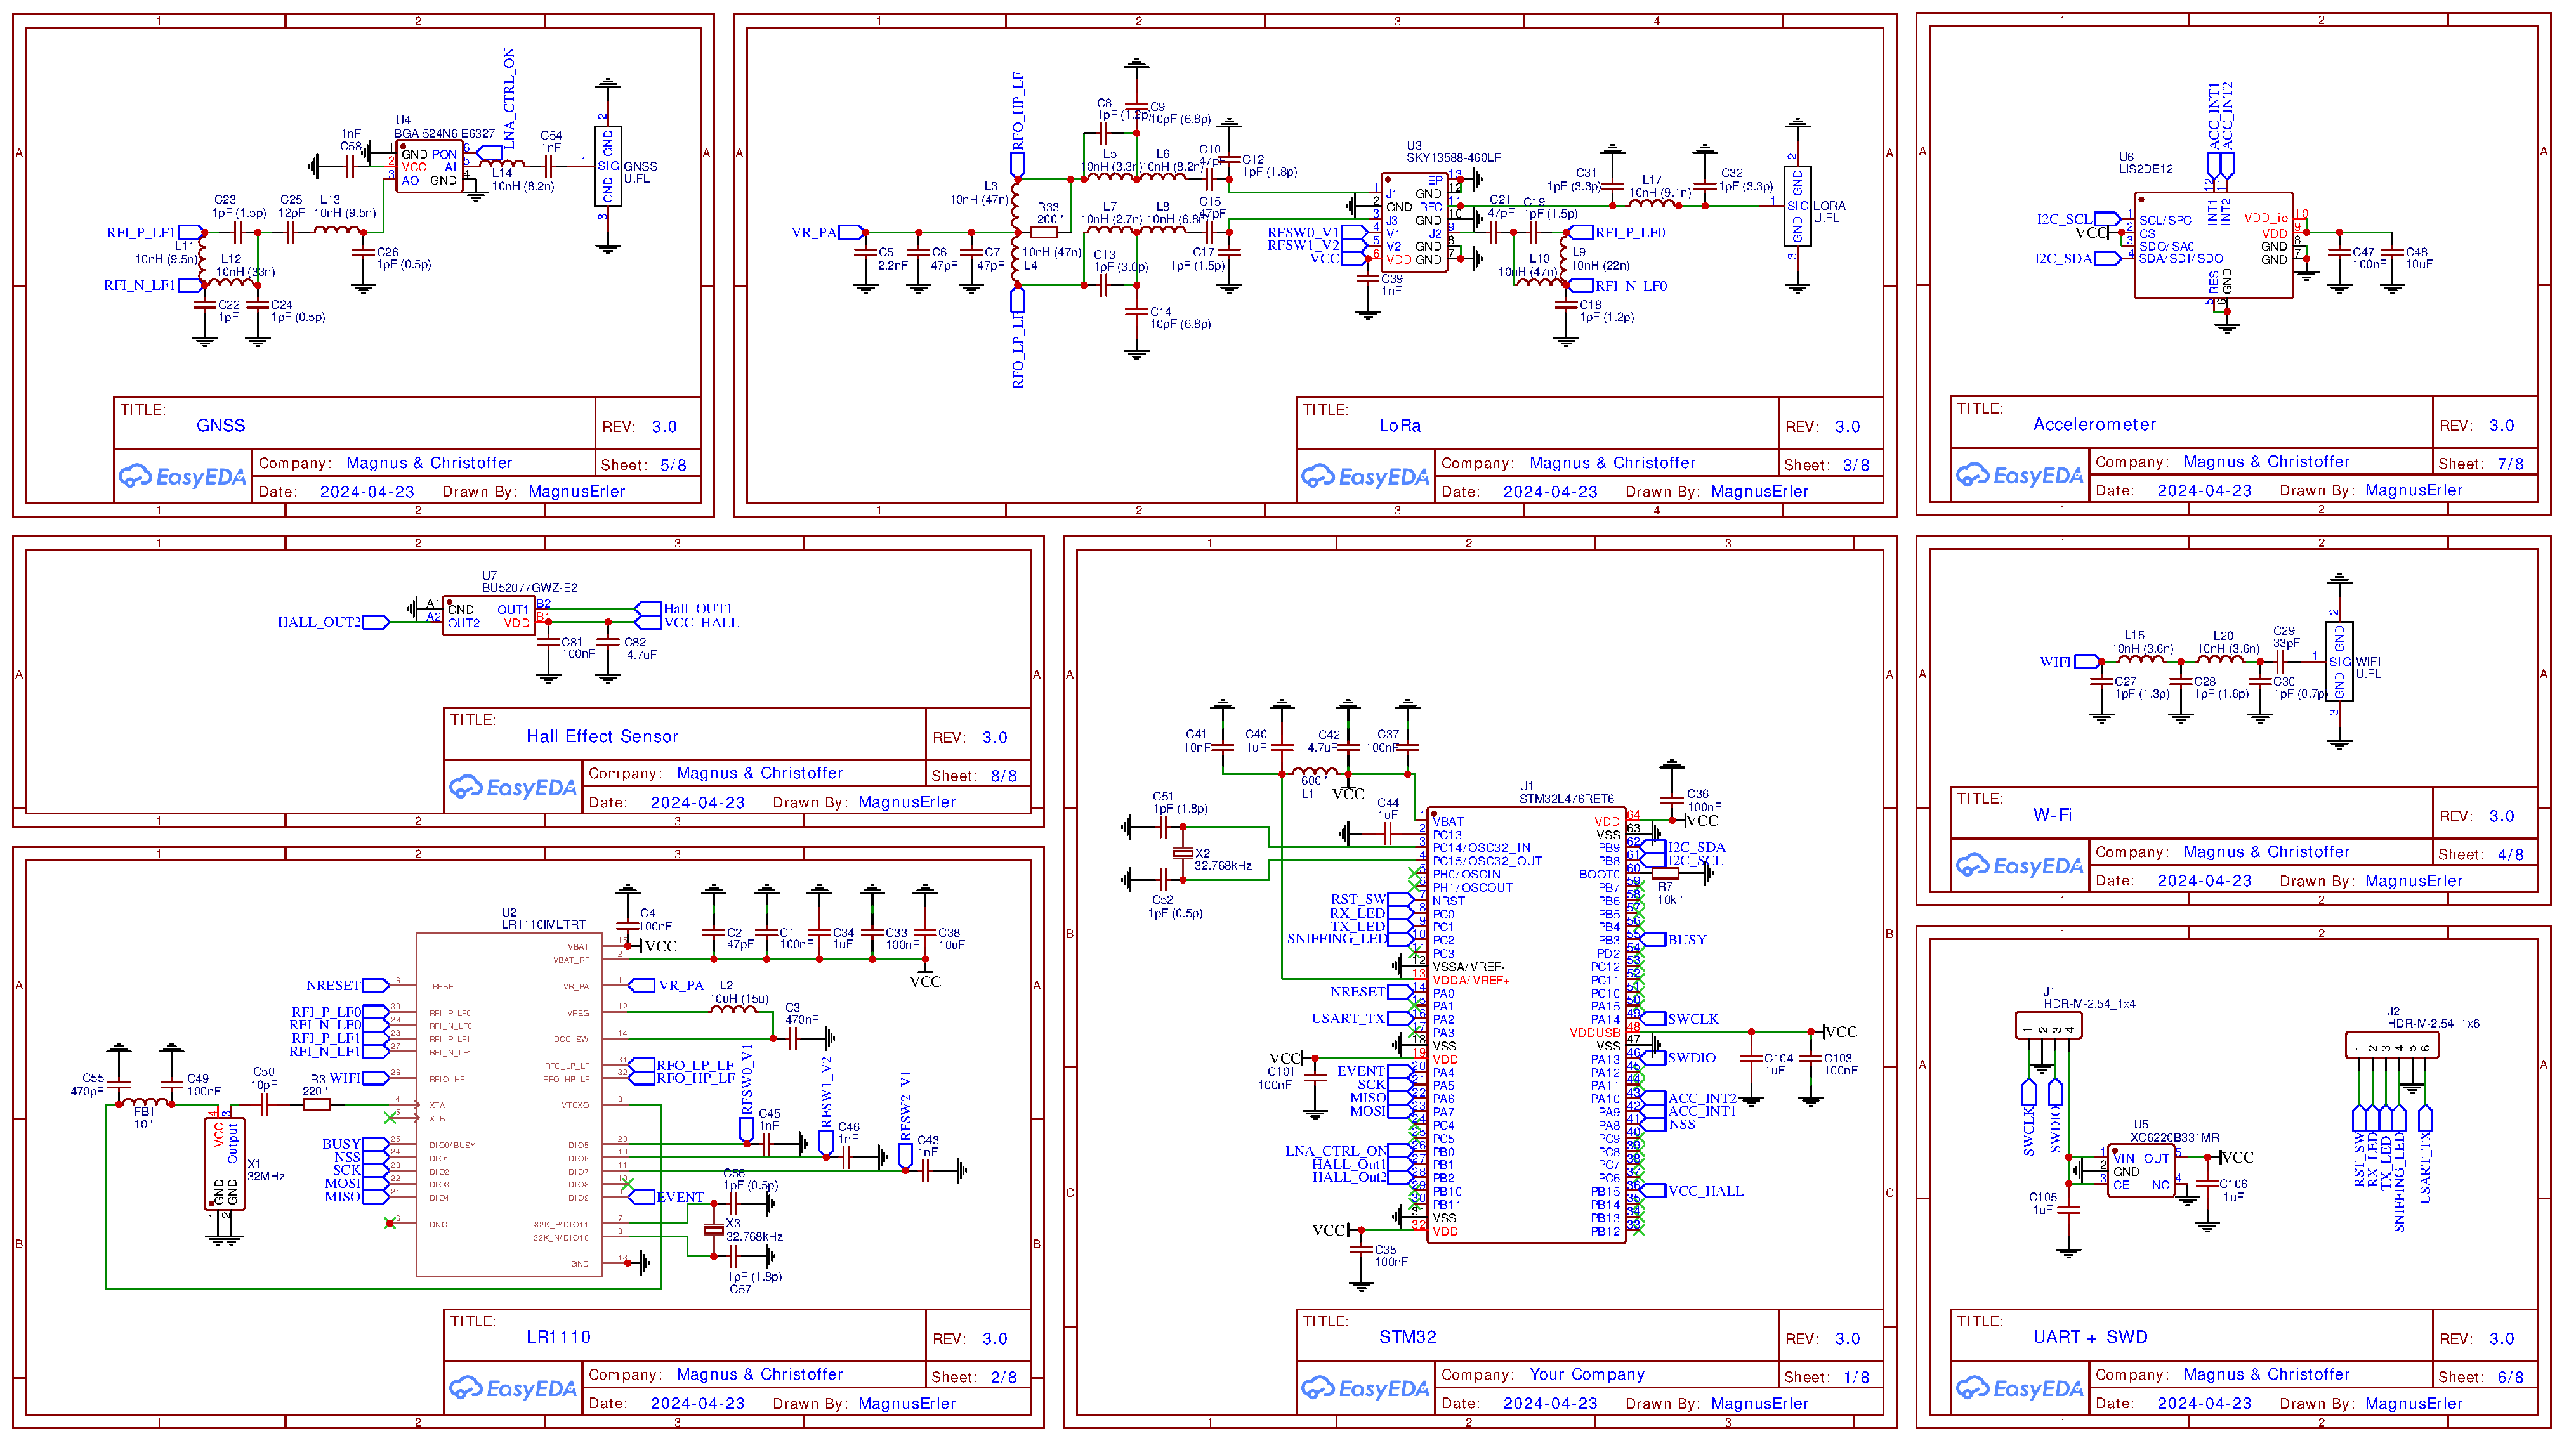
\includegraphics[width=1\textwidth]{figures/Schematic.pdf}
    \caption{Overview of the schematic. A larger schematic can be found in app.~\ref{app:wiringDiagram}.}
    \label{fig:schematic}
\end{figure}

\subsection{Case design}
We have set up requirements for this in the product requirements, so here you can say a little about how we prototype before the final design.
We have probably made several different prototypes. Chalk it up to the theory of prototypes.

\subsection{Cost}
LR1110 ordered from DigiKey Denmark\footnote{\url{https://www.digikey.dk/}} where it cost \SI{72.23}{\dkk} per chip. Ordering the rest from JLCPCB costs $\$2$ for the \ac{PCB} and an extra $\$35.61$ for the assembly of the components (5 \ac{PCB}). With shipping ($\$24.60$) and customs duties ($\$24.31$) the total amount is $\$86,52$. With the LR1110 chip, it is around \SI{193}{\dkk}.

The prices of key components are listed below in tab.~\ref{tab:BOM_keycomponents}. The rest of the \ac{BOM} in further detail can be viewed in app.~\ref{app:BOM}.

\begin{table}[H]
\centering
\small
\caption{BOM of key components.}
\label{tab:BOM_keycomponents}
\begin{tabular}{l|l|l|l|l|l}
Name & Designator & Footprint & Manufacturer Part & Manufacturer & Price [\$] \\ \hline
STM32L476 & U1 & LQFP-64 & STM32L476RET6 & ST & 2.924 \\
LR1110 & U2 & QFN-50 & LR1110IMLTRT & Semtech & 10.54 \\
SKY13588-460LF & U3 & QFN-12 & SKY13588-460LF & SKYWORKS & 2.254 \\
BGA524N6E6327 & U4 & TSNP-6 & BGA 524N6 E6327 & Infineon & 0.286 \\
XC6220B331MR & U5 & SOT23-5 & XC6220B331MR & TECH PUBLIC & 0.179 \\
LIS2DE12TR & U6 & LGA-12 & LIS2DE12TR & ST & 0.469 \\
BU52077GWZ-E2 & U7 & BGA-4 & BU52077GWZ-E2 & ROHM & 0.177 \\
\end{tabular}
\end{table}

\subsection{LoRaWAN communication}
Sending data from the Wi-Fi and \ac{GNSS} scans to the cloud is done through \ac{LoRaWAN}. The data is sent to the \ac{LoRaWAN} network server, which then forwards the data to the application server. The application server can then present the data in a user-friendly way. Sending the payload consumes a lot of power, so we have implemented power-saving features to only send the payload when the device has moved.

Suppose the accelerometer has not detected any movement in the period specified in the Wi-Fi or GNSS scan period. In that case, the device does not send the \ac{MAC} addresses of the Wi-Fi \ac{AP}s or \ac{GNSS} satellites. This would mean that the device has not moved and an additional scan for location is not necessary. Instead, it goes into sleep and checks again after either the Wi-Fi or \ac{GNSS} scan period has ended.

\subsubsection{Uplink communication}
If using Wi-Fi, each found\ac{MAC} address is appended and sent as one long payload on \ac{FPORT} 197. E.g. \texttt{00 2A 10 F4 A7 90 AA 8A FF 70 7E ED 6C 8B D3 CC F7 E0\textsubscript{(16)}} is a combination of \ac{MAC} address: \texttt{00 2A 10 F4 A7 90\textsubscript{(16)}}, \texttt{AA 8A FF 70 7E ED\textsubscript{(16)}}, and \texttt{6C 8B D3 CC F7 E0\textsubscript{(16)}}.

If using \ac{GNSS} the device sends XXX as a \ac{NAV} on \ac{FPORT} 198 or 192 depending on how many \ac{SV}'s the device can see

Setting it to \lstinline[style=C++]{SMTC_MODEM_SEND_MODE_STORE_AND_FORWARD} instead of normal \lstinline[style=C++]{SMTC_MODEM_SEND_MODE_UPLINK} will store the data in the LR1110 and send it when the device is in range of a \ac{LoRaWAN} gateway.

Tab.~\ref{tab:uplink_commands} shows the uplink commands that can be sent to the device.

\begin{table}[H]
\centering
\caption{Uplink commands.}
\label{tab:uplink_commands}
\begin{tabular}{l|l|l}
\ac{FPORT} & Usage & Payload \\ \hline
3 & Get temperature, battery voltage, and uptime & E.g. $26.4$ and $3.3$ \\
5 & Get firmware version & \\
6 & Get \ac{JoinEUI} & \\
7 & Get \ac{DevEUI} & \\
199 & LoRa Cloud requests (aka DM port or Stream port) & \\
201 & fragport & \\
\end{tabular}
\end{table}

The power consumption in sending 1 byte or 4 bytes over \ac{LoRaWAN} is not substantial


\subsubsection{Downlink communication}
Data from \ac{GNSS} can either be sent with \ac{GNSS} or \ac{GNSSNG}. \ac{GNSSNG} is used for multiple NAV messages.

Tab.~\ref{tab:downlink_commands} shows the downlink commands that can be sent to the device.

\begin{table}[H]
\centering
\caption{Downlink commands.}
\label{tab:downlink_commands}
\begin{tabular}{l|l|p{9cm}|l}
\ac{FPORT} & Payload & Usage & Default \\ \hline
1 & Scan period & \ac{GNSS} scan period [s] & \SI{120}{\second} \\
2 & Scan period & Set Wi-Fi scan period [s] & \SI{60}{\second} \\
192 & & \ac{GNSSNG}  & \\
197 & & Wi-Fi scan results to be forwarded to LoRa Cloud & \\
198 & & \ac{GNSS} port  & \\
199 & & LoRa Cloud requests ----- DM port ----- Stream port  & \\
201 & & fragport  & \\
\end{tabular}
\end{table}
% https://tektelic.com/wp-content/uploads/TEKTELIC_STORK_UG.pdf page 11
% https://www.chirpstack.io/docs/chirpstack/integrations/loracloud.html

Need to have:
Downlink
\ac{GNSS} scan interval
Wi-Fi scan interval

Uplink
Battery critical

Nice to have
Downlink
Temperature
Battery status

\subsection{Application}

ngrok\footnote{\url{https://ngrok.com/}}

One predominant requirement derived from our interviews was the need for a simple setup process for our device and an easy-to-use application for presenting the data.
Despite the growing adoption of \ac{LoRaWAN}-enabled devices, network setup remains considerably more intricate than devices that utilise Wi-Fi or cellular networks for data transmission which mostly work out of the box. Wi-Fi devices merely require access to an access point and a network password, and cellular devices only necessitate a SIM card, where the technical part of joining the network is left to the network provider. \ac{LoRaWAN}-enabled device on the other hand entails several additional considerations. You need to think about provisioning, choice of network and network coverage, network protocol version and regional requirements.

Let us look at how one would add an LR1110 end device to the network and start getting geolocation pings
\begin{enumerate}
    \item Get device info from the chip (\ac{DevEUI}, PIN and \ac{JoinEUI})
    \item Create a user on Loracloud.com 
    \item Create an application on Loracloud.com
    \item Choose the \ac{LoRaWAN} network provider or implement your own gateway
    \item Change bindings for Loracloud.com application to allow join requests from chosen \ac{LoRaWAN} network provider
    \item Claim device on Loracloud.com Join Server
    \item Claim device on Loracloud.com Modem \& Geolocation Services
    \item Create user at chosen \ac{LoRaWAN} network provider
    \item Create application at chosen \ac{LoRaWAN} network provider
    \item Register device at chosen \ac{LoRaWAN} network provider with correct frequency plan, \ac{LoRaWAN} version, regional parameters, \ac{JoinEUI} and \ac{DevEUI}
    \item Create API token on Loracloud.com Modem \& Geolocation Services
    \item Setup integration between \ac{LoRaWAN} network provider application and Loracloud.com Modem \& Geolocation Services.
\end{enumerate}

Looking at the above list, one can see that setting up an LR1110 device is a technical ?

We therefore chose to make our application setup less technical and provide a more coherent and easy-to-use user experience.

Setup for our application:
1. Read \ac{DevEUI}, PIN on the package.
2. 
3.
4.
5.
6.
7.
8.

If a new location has been found but it is close to the previous lcoation (e.g. radius of \SI{5}{\meter}) that location will not be shown on the map, but however updated as the device has been seen.

Future work:
Låst til TheThingsNetwork
Låst til EU
Stadig lidt teknisk. Man skal finde application keys og certificate

When developing a web application, there is no need to reinvent the wheel and code everything from scratch. One could use technologies such as vanilla HTML, CSS and JavaScript, however using a front-end framework or library as a scaffold for building your application, offers enhanced efficiency, consistency and scalability. Frameworks provide a standardised structure with easier maintainability and features like cross-browser compatibility, strong community support, and built-in security.

\subsubsection{Client-side}
Many different frameworks or libraries could have been chosen for the client side of our application. We chose React as we have prior experience with it and its prominence as one of the most used web technologies (source: \url{https://survey.stackoverflow.co/2023/#technology-most-popular-technologies}), offered extensive availability of libraries, online resources and community support.
Leaflet\footnote{\url{https://leafletjs.com/}} was chosen for displaying the map, as it is the leading open-source JavaScript library for mobile-friendly interactive maps. We could have chosen to use Google's map service, as it would have offered familiarity (a wish we saw in our interviews). However this service isn't free, and will therefore add a cost to the product, and the price was the bigger factor for all users, and the interaction with Leaflet is quite similar to how you interact with Google Maps.

\subsubsection{Server-side}
Express
SQLite3
\newpage
\section{Testing and validation of the design } \label{sec:testing}

The design and its implementation have been thoroughly tested.

\subsection{Possible test scenarios}
\begin{enumerate}
    \item Test if it uses less power to have a timer on STM that turns the accelerometer on and off
    \item Which temperature sensor uses less power?
    \item VBAT can be measured from STM and LR-chip
    \item Does the accelerometer use more power when reading temp?
    \item Send VBat and temp with each upload to TTN?
    \item How much power does it use to set all registers at once or one after one in the accelerometer
    \item Does it make sense to use power-down mode instead of \SI{1}{\hertz}?
\end{enumerate}

\subsection{Testing method - Statistics}
Method section on testing. Brief statistics

\subsection{Accuracy}
\ac{GNSS} accuracy is measured in meters and describes the difference between the physical location of the device with the location that the device reports.
How accurate are the different methods? What is our uncertainty?

Testing the accuracy is done by looking at the accuracy value of the GPS module, and performing tests where we compare the device's physical location with the location that the device reports.

\subsection{Power consumption}
How much power the device uses in the different modes

We used the Power Profiler Kit II\footnote{\url{https://www.nordicsemi.com/Products/Development-hardware/Power-Profiler-Kit-2}} from Nordic Semiconductor to measure the device's power consumption.

Power Profiler v4.0.0

To visualise the data we used the app Power Profiler from nRF Connect for Desktop\footnote{\url{https://www.nordicsemi.com/Products/Development-tools/nRF-Connect-for-Desktop}} which also is a tool from Nordic Semiconductor.

\subsection{Results according to design/performance criteria}
How does the product meet our design criteria

\subsection{LTE-M vs NB-IOT vs LoRaWAN}

\begin{table}[H]
\centering
\caption{\url{https://www3.cs.stonybrook.edu/~mdasari/courses/cse570/lora.pdf}}
\begin{tabular}{lll}
              & LoRaWAN    & NB-IoT    \\
TX Current    & 24-\SI{44}{\milli\ampere} & 74-\SI{220}{\milli\ampere} \\
RX Current    & \SI{12}{\milli\ampere}     & \SI{46}{\milli\ampere}     \\
Idle Current  & \SI{1.4}{\milli\ampere}     & \SI{6}{\milli\ampere}      \\
Sleep Current & \SI{0.1}{\micro\ampere} & \SI{3}{\micro\ampere}
\end{tabular}
\end{table}


\newpage
\section{Conclusion and suggestions for future research} \label{sec:conclusion}

The project has been a challenging task with many decisions to consider. It could be demonstrated that


\subsection{Future work}

What about LR1120? Why not use that chip?


Why the Lr1110 chip? And not LR1112 or another chip?


The next generation of dementia patients will use smartphones as this is what they are familiar with.

Length vs width. What is better? Should it be squared or longer and less wide?

This is proof of concept. Den endelige udformning skal laves i samarbejde med partner

Different GNSS module: TESEO-LIV3R

https://blues.com/blog/network-connectivity/


The stm32 chip as an infrared: 3.24.5 Infrared interface


\begin{itemize}
  \item Mobile application: Create a mobile app where the user can configure tracker settings. E.g. setting the phone's hotspot (Wi-Fi) to a specific \ac{SSID} (service set identifier), that will be picked up by the tracker, which then goes into a mode where it can change settings. We don't know yet how to send data to the tracker (maybe over Wi-Fi)
\end{itemize}
\newpage
\iffalse
\begin{table}[H]
\centering
\caption{Gantt schedule.}
\label{tab:rosNode}
\begin{tabular}{p{0.30\textwidth}
!{\vrule width 0.4mm}p{0.0013\textwidth}*{3}{|p{0.0013\textwidth}}
!{\vrule width 0.4mm}p{0.0013\textwidth}*{3}{|p{0.0013\textwidth}}
!{\vrule width 0.4mm}p{0.0013\textwidth}*{3}{|p{0.0013\textwidth}}
!{\vrule width 0.4mm}p{0.0013\textwidth}*{3}{|p{0.0013\textwidth}}
!{\vrule width 0.4mm}p{0.0013\textwidth}*{3}{|p{0.0013\textwidth}}
!{\vrule width 0.4mm}p{0.0013\textwidth}*{3}{|p{0.0013\textwidth}}
|}
% The top line
\textbf{Month} 
            & \multicolumn{4}{c!{\vrule width 0.4mm}}{Jan} 
            & \multicolumn{4}{c!{\vrule width 0.4mm}}{Feb} 
            & \multicolumn{4}{c!{\vrule width 0.4mm}}{Mar} 
            & \multicolumn{4}{c!{\vrule width 0.4mm}}{Apr} 
            & \multicolumn{4}{c!{\vrule width 0.4mm}}{May} 
            & \multicolumn{4}{c|}{June} \\
% The second line, with its five years of four quarters
%\rpt[5]{& 1 & 2 & 3 & 4} \\
\hline
% using the on macro to fill in twenty cells as `on'
Setting up development environment        \offr[3] \on[2] \off[19]\\
\hline
Establishing contact with the LR1110 chip    \offr[3] \on[3] \off[18]\\
\hline
Write status report    \offr[3] \off[21] \\
\hline
Exploring LR1110 commands    \offr[3] \off[21] \\
\hline
Reading up on WiFi \& GNSS tracking    \offr[3] \off[21] \\
\hline
Write theory section on WiFi, GNSS \& SPI   \offr[3] \off[21] \\
\hline
Implement WiFi scanner     \offr[3] \off[21] \\
\hline
Implement LoRaWAN     \offr[3] \off[21] \\
\hline
Implement Satellite scanner     \offr[3] \off[21] \\
\hline
Write section about tracking   \offr[3] \off[21] \\
\hline
Investigate power use    \offr[3] \off[21] \\
\hline
Write section about initial power use    \offr[3] \off[21] \\
\hline
Discuss product requirements with potential users    \offr[3] \off[21] \\
\hline
Put together product requirements    \offr[3] \off[21] \\
\hline
Write section about product requirements    \offr[3] \off[21] \\
\hline
Design product according to product requirements    \offr[3] \off[21] \\
\hline
Write product development section    \offr[3] \off[21] \\
\hline
Test product according to product requirements    \offr[3] \off[21] \\
\hline
Finalise report in LaTeX    \offr[3] \off[21] \\
\hline
Beautify report    \offr[3] \off[21] \\
\hline
% using the on macro followed by the off macro
Defence preparation     \offr[3] \off[16] \on[5]\\
\hline
% The mbox prevent packages from being hyphenated
% The multicolumn produces no vertical guides within the columns it spans, but
% does put one at the end to complete the right-hand edge of the table
\end{tabular}
\end{table}
\fi

%Proptype development
%Proptype testing
%Techinal report


\begin{landscape}
    %\subsection*{Timeschedule}
    \Large{\textbf{Timeschedule}}
    \begin{table}[H]
    \tiny
    \centering
    \caption[Timeschedule shown as a Gantt chart]{\footnotesize{Timeschedule shown as a Gantt chart. The tasks responsible are divided by colour; \textcolor{blue!90}{blue for both}, \textcolor{green!90}{green for Christoffer}, and \textcolor{red!90}{red for Magnus}.}}
    \begin{tabular}{|p{5.0cm}|*{23}{p{0.3cm}|}}
    \hline
    \textbf{Month} & \multicolumn{1}{c}{\textbf{Jan}} & \multicolumn{4}{c}{\textbf{Feb}} & \multicolumn{5}{c}{\textbf{March}} & \multicolumn{4}{c}{\textbf{April}} & \multicolumn{4}{c}{\textbf{May}} & \multicolumn{5}{c|}{\textbf{June}} \\ \hline
    Week & 4 & 5 & 6 & 7 & 8 & 9 & 10 & 11 & 12 & 13 & 14 & 15 & 16 & 17 & 18 & 19 & 20 & 21 & 22 & 23 & 24 & 25 & 26 \\ \hline
    \multicolumn{24}{c}{\textbf{Planning}} \\ \hline
    Set up development environment                      & \ccellThree{blue} & & & & & & & & & & & & & & & & & & & & \\ \hline
    Implement connection with the LR1110 chip           & & \cellThree{red} & & & & & & & & & & & & & & & & & & & \\ \hline
    Write status report                                 & & & \cellThree{blue} & & & & & & & & & & & & & & & & & & \\ \hline
    \multicolumn{24}{c}{\textbf{Litterateur review and research}} \\ \hline
    Explore LR1110 commands                             & & & & \cellTwo{blue} & & & & & & & & & & & & & & & & & & \\ \hline
    Read about WiFi and GNSS tracking                   & & & & & \cellTwo{blue} & & & & & & & & & & & & & & & & & \\ \hline
    Write section on WiFi, GNSS, LoRaWAN and SPI        & & & & & \cellTwo{white} & & & & & & & & & & & & & & & & & \\ \hline
    \multicolumn{24}{c}{\textbf{Prototype development}} \\ \hline
    Implement WiFi scanner                              & & & & & \cellFour{white} & & & & & & & & & & & & & & & \\ \hline
    Implement LoRaWAN                                   & & & & & \cellFour{white} & & & & & & & & & & & & & & & \\ \hline
    Implement Satellite scanner                         & & & & & \cellFour{white} & & & & & & & & & & & & & & & \\ \hline
    Write section about tracking                        & & & & & & \cellThree{white} & & & & & & & & & & & & & & & \\ \hline
    Design product according to product requirement     & & & & & & & & & & & \CellFive{white} & & & & & & & & \\ \hline
    \multicolumn{24}{c}{\textbf{Design requirements}} \\ \hline
    Short market analysis/overview   & & & & & & & \cellOne{white} & & & & & & & & & & & & & & & & \\ \hline
    Brainstorm use cases   & & & & & & & \cellOne{white} & & & & & & & & & & & & & & & & \\ \hline
    Write initial design requirements   & & & & & & & \CellTwo{white} & & & & & & & & & & & & & & & \\ \hline
    Discuss product requirements with potential users   & & & & & & & & \cellTwo{white} & & & & & & & & & & & & & & \\ \hline
    Put together product requirements   & & & & & & & & & \cellTwo{white} & & & & & & & & & & & & & \\ \hline
    Write section about product requirements            & & & & & & & & & & \cellOne{white} & & & & & & & & & & & & & \\ \hline
    \multicolumn{24}{c}{\textbf{Prototype testing}} \\ \hline
    Test product according to product requirements      & & & & & & & & & & & & & & & \CellFour{white} & & & & & \\ \hline
    \multicolumn{24}{c}{\textbf{Technical report}} \\ \hline
    Finalise report in LaTeX                            & & & & & & & & & & & & & & & & & & \cellFour{blue} & & \\ \hline
    Proofreading                                        & & & & & & & & & & & & & & & & & & & & & & \cellOne{blue} & \\ \hline
    Transfer report to InDesign                         & & & & & & & & & & & & & & & & & & & & & \cellTwo{green} & \\ \hline
    Prepare for defence                                 & & & & & & & & & & & & & & & & & & & & & & \cellTwo{blue} \\ \hline
    \end{tabular}
    \normalsize
    \end{table}
\end{landscape}
\newpage
\addcontentsline{toc}{section}{References}
%\bibliographystyle{apalike}
\bibliographystyle{abbrvnat}
%\bibliographystyle{IEEEtr}
\bibliography{ref}
\newpage
\begin{appendices}
\addtocontents{toc}{\protect\setcounter{tocdepth}{0}} % Suppress sub-levels in TOC within appendices


\section{Development setup} \label{app:devsetup}
If working on Windows, the following programs are needed:
\begin{itemize}
    \item CubeMX \ref{app:software:stm32cubemx}
    \item Arm GNU Toolchain (download as zip) \ref{app:software:arm_toolchain}
    \item Visual Studio Code \ref{app:software:vsc}
    \item OpenOCD \ref{app:software:openocd}
    \item Git (download as zip) \ref{app:software:git}
\end{itemize}

And the following binaries:
\begin{itemize}
    \item Make for Windows with dependencies \ref{app:software:make}
\end{itemize}

\begin{enumerate}
    \item Download all of the files, install VSCode and CubeMX and unpack the rest to a folder of your choice.
    \item Setup a new project in CubeMX, and change the toolchain under the project manager to \lstinline[style=bash]{Makefile}
    \item Add paths to system environment variables.
    \begin{enumerate}
        \item Add new variable with name \lstinline[style=bash]{ARMGCC\_DIR} with value \lstinline[style=bash]{<your path>\arm-gnu-toolchain-<version>.Rel1-mingw-w64-i686-arm-none-eabi\bin}
        \item Edit path variable and add:
        \begin{enumerate}
            \item \lstinline[style=bash]{\%ARMGCC\_DIR\%}
            \item \lstinline[style=bash]{<your path>\make-<version>\bin}
            \item \lstinline[style=bash]{<your path>\OpenOCD-<version>\bin}
            \item \lstinline[style=bash]{<your path>\git\bin}
            \item \lstinline[style=bash]{<your path>\git\usr\bin}
        \end{enumerate}
    \end{enumerate}
    \item Open a new terminal and test that the environment variables are set correctly by running \lstinline[style=bash]{make --version}, \lstinline[style=bash]{openocd --version}, \lstinline[style=bash]{git --version} and \lstinline[style=bash]{arm-none-eabi --version}. If every command returns a version number, your environment variables have been updated correctly.
    \item Test that you can compile, by going into your newly created project directory and running the command \lstinline[style=bash]{make}.
    If no error appears, a hex and bin-file are created inside the newly created folder: \lstinline[style=bash]{...\build\<project-name>.hex}.
    \item Open the newly created \lstinline[style=bash]{Makefile} and add the following:
    \begin{lstlisting}[style=bash]
        #######################################
        # openocd
        #######################################
        flash: all
       openocd -f interface/stlink.cfg -f target/@board version@.cfg -c "program $(BUILD_DIR)/$(TARGET).elf verify reset exit"
    \end{lstlisting}
    where the corresponding cfg file for your board, should be found in: \\ 
    \lstinline[style=bash]{<your path>\OpenOCD-<version>\share\openocd\scripts\target}
    \item You should now be able to flash the board by running the command \lstinline[style=bash]{make flash} in a terminal in the project directory.
 \end{enumerate}



Another way to set this up on Windows is to use \ac{WSL}.

%\textcolor{red}{Hvis man gør dette, skal man også bruge VSCode gennem WSL. Det har vi ikke prøvet endnu, men det burde jo egentlig virke}

If working on a Windows machine, open PowerShell and run the following to install \ac{WSL} \sbref{app:software:wsl}.
\begin{lstlisting}[style=bash]
sudo apt update && sudo apt upgrade
wsl --install
\end{lstlisting}
The machine is now set up like a Linux machine and can perform alike.

To fetch, compile and run the firmware code in the GitHub repository, the user needs to install Git \sbref{app:software:git}, GNU Make \sbref{app:software:make}, ARM GNU Toolchain \sbref{app:software:arm_toolchain}, and OpenOCD \sbref{app:software:openocd}.
\begin{lstlisting}[style=bash]
sudo apt install git make gcc-arm-none-eabi openocd
\end{lstlisting}

When installed, the GitHub repository \sbref{app:code} can be cloned\footnote{Cloning a repository: \url{https://docs.github.com/en/repositories/creating-and-managing-repositories/cloning-a-repository}} to a desired directory, and the development can start using an \ac{IDE}.

\subsection{Visual Studio Code integration}
The preferred \ac{IDE} used in this project is Visual Studio Code \sbref{app:software:vsc}. Open the newly cloned repository and, if in Windows, run in the terminal \lstinline[style=bash]{wsl} to start performing like a Linux machine.

The compiling of the project is based on a simple makefile and can be compiled with:
\begin{lstlisting}[style=bash]
make
make -f CustomeNameMakefile     # used for custom names
\end{lstlisting}
If no error appears, a hex-file is created inside the newly created folder (\lstinline[style=bash]{build\VSC_win.hex}), and can be flashed to the STM32 chip with \lstinline[style=bash]{make flash}.

For debugging, install Cortex-Debug \sbref{app:software:cortex_debug} in the Extension Marketplace.

Create a new folder called ".vscode" for personal setup of the debugging and running of the code and add two files from appendix \sbref{app:software:c_cpp_properties} and \sbref{app:software:launch}.

\section{Code} \label{app:code}
All code is available on GitHub at \url{https://github.com/MagnusErler/WiFiLocationTracker}.\\
Update firmware: \url{https://github.com/Lora-net/lr1110_updater_tool/wiki}\\
\url{https://github.com/Lora-net/SWTL001/wiki}

\section{Essential hardware} \label{app:hardware}
\begin{enumerate}
    \item LR1110 : \url{https://www.semtech.com/products/wireless-rf/lora-edge/lr1110} \label{app:hardware:lr1110}
    \item STM32L476RG : \url{https://www.st.com/en/microcontrollers-microprocessors/stm32l476rg.html} \label{app:hardware:stm32l476rg}
    \item NT2016SA 32MHz END4263A : \url{https://www.digikey.dk/en/products/detail/ndk-america-inc/NT2016SA-32M-END4263A/8275433} \label{app:hardware:tcxo}
    \item LIS2DE12 : \url{https://www.st.com/resource/en/datasheet/lis2de12.pdf} \label{app:hardware:lis2de12}
    \item BU52077GWZ : \url{https://fscdn.rohm.com/en/products/databook/datasheet/ic/sensor/hall/bu52077gwz-e.pdf} \label{app:hardware:BU52077GWZ}
    \item XC6220B331MR : \url{https://product.torexsemi.com/system/files/series/xc6220.pdf} \label{app:hardware:XC6220}
    \item BGA524N6E6327 : \url{https://www.infineon.com/dgdl/Infineon-BGA524N6-DataSheet-v03_05-EN.pdf?fileId=db3a304344e406b50144e44dfad302b9} \label{app:hardware:bga524n6e6327}
\end{enumerate}

\section{Essential software}  \label{app:software}
\begin{enumerate}
    \item Visual Studio Code : \url{https://code.visualstudio.com/} \label{app:software:vsc}
    \item STM32CubeMX : \url{https://www.st.com/content/st_com/en/stm32cubemx.html} \label{app:software:stm32cubemx}
    \item Git : \url{https://git-scm.com/} \label{app:software:git}
    \item GNU Make : \url{https://gnuwin32.sourceforge.net/packages/make.htm} \label{app:software:make}
    \item ARM GNU Toolchain : \url{https://developer.arm.com/downloads/-/gnu-rm}
    https://developer.arm.com/downloads/-/gnu-rm
    \label{app:software:arm_toolchain}
    \item OpenOCD : \url{https://gnutoolchains.com/arm-eabi/openocd/} \label{app:software:openocd}
    \item Cortex-Debug : \url{https://marketplace.visualstudio.com/items?itemName=marus25.cortex-debug} \label{app:software:cortex_debug}
    \item WSL : \url{https://learn.microsoft.com/en-us/windows/wsl/install} \label{app:software:wsl}
    \item AppCAD : \url{https://www.broadcom.com/info/wireless/appcad} \label{app:software:appcad}
\end{enumerate}

And the following binaries:
- Make for Windows with dependencies \url{https://gnuwin32.sourceforge.net/packages/make.htm} 

\section{Windows and Linux setup}
\subsection*{\lstinline[style=bash]{c_cpp_properties.json}} \label{app:software:c_cpp_properties}
\begin{lstlisting}[language=json]
{
    "configurations": [
        {
            "name": "STM32L476RG",
            "includePath": [
                "${workspaceFolder}/**",
                "${workspaceFolder}/Src/radio/lr1110_modem/src"
            ],
            "defines": [
                "USE_HAL_DRIVER",
                "STM32L476xx"
            ],
            "configurationProvider": "ms-vscode.makefile-tools",
            "compilerPath": "C:/Program Files (x86)/Microsoft Visual Studio/2022/BuildTools/VC/Tools/MSVC/14.38.33130/bin/Hostx64/x64/cl.exe", // Use "which arm-none-eabi-gcc" to get the location of the compiler in linux
            "compilerArgs": [
                "-mcpu=cortex-m4",
                "-mthumb"
            ],
            "cStandard": "c11",
            "cppStandard": "c++17"
        }
    ],
    "version": 4
}
\end{lstlisting}

\subsection*{\lstinline[style=bash]{launch.json}} \label{app:software:launch}
\begin{lstlisting}[language=json]
{
    "version": "0.2.0",
    "configurations": [
        {
            "name": "Cortex Debug",
            "cwd": "${workspaceFolder}",
            "executable": "./build/VSC_win.elf",
            "request": "launch",
            "type": "cortex-debug",
            "runToEntryPoint": "main",
            "servertype": "openocd",
            "device": "STM32L476RG",
            "configFiles": [
                "interface/stlink.cfg",
                "target/stm32l4x.cfg"
            ]
        }
    ]
}
\end{lstlisting}

\section{PCB}

\subsection{BOM} \label{app:BOM}

\begin{footnotesize}
\begin{longtable}{llllll}
    \caption{BOM of the tracker.} \\
    \toprule
    Name & Designator & Footprint & Manufacturer Part & Manufacturer & Price [\$] \\
    \midrule
    \endfirsthead
    
    \multicolumn{6}{c}{\normalsize{\tablename\ \thetable{} BOM.}} \\
    \toprule
    Name & Designator & Footprint & Manufacturer Part & Manufacturer & Price [\$] \\
    \midrule
    \endhead
    
    %\bottomrule
    %\multicolumn{6}{r}{{Continued on next page}} \\
    \endfoot
    
    %\bottomrule
    \endlastfoot

    \multicolumn{6}{c}{\cellcolor[HTML]{EFEFEF}Chips} \\
    STM32L476 & U1 & LQFP-64 & STM32L476RET6 & ST & 2.924 \label{bom:stm32l476} \\
    LR1110 & U2 & QFN-50 & LR1110IMLTRT & Semtech & 10.54 \label{bom:lr1110}\\
    SKY13588-460LF & U3 & QFN-12 & SKY13588-460LF & SKYWORKS & 2.254 \\
    BGA524N6E6327 & U4 & TSNP-6 & BGA524N6E6327 & Infineon & 0.286 \label{bom:bga524n6e6327}\\
    XC6220B331MR & U5 & SOT23-5 & XC6220B331MR & TECH PUBLIC & 0.179 \label{bom:xc6220} \\
    LIS2DE12TR & U6 & LGA-12 & LIS2DE12TR & ST & 0.469 \label{bom:lis2de12}\\
    BU52077GWZ-E2 & U7 & BGA-4 & BU52077GWZ-E2 & ROHM & 0.177 \label{bom:bu52077gwz}\\

    \multicolumn{6}{c}{\cellcolor[HTML]{EFEFEF}Resistors} \\
    \SI{220}{\ohm} & R3 & R0402 & 0402WGF2200TCE & UNI-ROYAL & 0.001 \\
    \SI{10}{\kilo\ohm} & R7 & R0402 & 0402WGF1002TCE & UNI-ROYAL & 0.001 \\
    \SI{200}{\ohm} & R33 & R0603 & 0603WAF2000T5E & UNI-ROYAL & 0.001 \\

    \multicolumn{6}{c}{\cellcolor[HTML]{EFEFEF}Capacitors} \\
    \SI{100}{\nano\farad} & C1 & C0402 & CL05B104KO5NNNC & SAMSUNG & 0.001 \\
    \SI{47}{\pico\farad} & C2 & C0402 & 0402CG470J500NT & FH & 0.001 \\
    \SI{470}{\nano\farad} & C3 & C0603 & CL10B474KA8NNNC & SAMSUNG & 0.007 \\
    \SI{100}{\nano\farad} & C4 & C0402 & CL05B104KO5NNNC & SAMSUNG & 0.001 \\
    \SI{2.2}{\nano\farad} & C5 & C0603 & 0603B222K500NT & FH & 0.002 \\
    \SI{47}{\pico\farad} & C6 & C0402 & 0402CG470J500NT & FH & 0.001 \\
    \SI{47}{\pico\farad} & C7 & C0402 & 0402CG470J500NT & FH & 0.001 \\
    \SI{1}{\pico\farad} (1.2p) & C8 & C0402 & 0402CG1R0C500NT & FH & 0.001 \\
    \SI{10}{\pico\farad} (6.8p) & C9 & C0402 & CL05C100JB5NNNC & SAMSUNG & 0.005 \\
    \SI{47}{\pico\farad} & C10 & C0402 & 0402CG470J500NT & FH & 0.001 \\
    \SI{1}{\pico\farad} (1.8p) & C12 & C0402 & 0402CG1R0C500NT & FH & 0.001 \\
    \SI{1}{\pico\farad} (3.0p) & C13 & C0402 & 0402CG1R0C500NT & FH & 0.001 \\
    \SI{10}{\pico\farad} (6.8p) & C14 & C0402 & CL05C100JB5NNNC & SAMSUNG & 0.005 \\
    \SI{47}{\pico\farad} & C15 & C0402 & 0402CG470J500NT & FH & 0.001 \\
    \SI{1}{\pico\farad} (1.5p) & C17 & C0402 & 0402CG1R0C500NT & FH & 0.001 \\
    \SI{1}{\pico\farad} (1.2p) & C18 & C0402 & 0402CG1R0C500NT & FH & 0.001 \\
    \SI{1}{\pico\farad} (1.5p) & C19 & C0402 & 0402CG1R0C500NT & FH & 0.001 \\
    \SI{47}{\pico\farad} & C21 & C0402 & 0402CG470J500NT & FH & 0.001 \\
    \SI{1}{\pico\farad} & C22 & C0402 & 0402CG1R0C500NT & FH & 0.001 \\
    \SI{1}{\pico\farad} (1.5p) & C23 & C0402 & 0402CG1R0C500NT & FH & 0.001 \\
    \SI{1}{\pico\farad} (0.5p) & C24 & C0402 & 0402CG1R0C500NT & FH & 0.001 \\
    \SI{12}{\pico\farad} & C25 & C0402 & 0402CG120J500NT & FH & 0.001 \\
    \SI{1}{\pico\farad} (0.5p) & C26 & C0402 & 0402CG1R0C500NT & FH & 0.001 \\
    \SI{1}{\pico\farad} (1.3p) & C27 & C0402 & 0402CG1R0C500NT & FH & 0.001 \\
    \SI{1}{\pico\farad} (1.6p) & C28 & C0402 & 0402CG1R0C500NT & FH & 0.001 \\
    \SI{33}{\pico\farad} & C29 & C0402 & 0402CG330J500NT & FH & 0.001 \\
    \SI{1}{\pico\farad} (0.7p) & C30 & C0402 & 0402CG1R0C500NT & FH & 0.001 \\
    \SI{1}{\pico\farad} (3.3p) & C31 & C0402 & 0402CG1R0C500NT & FH & 0.001 \\
    \SI{1}{\pico\farad} (3.3p) & C32 & C0402 & 0402CG1R0C500NT & FH & 0.001 \\
    \SI{100}{\nano\farad} & C33 & C0402 & CL05B104KO5NNNC & SAMSUNG & 0.001 \\
    \SI{1}{\micro\farad} & C34 & C0402 & CL05A105KA5NQNC & SAMSUNG & 0.004 \\
    \SI{100}{\nano\farad} & C35 & C0402 & CL05B104KO5NNNC & SAMSUNG & 0.001 \\
    \SI{100}{\nano\farad} & C36 & C0402 & CL05B104KO5NNNC & SAMSUNG & 0.001 \\
    \SI{100}{\nano\farad} & C37 & C0402 & CL05B104KO5NNNC & SAMSUNG & 0.001 \\
    \SI{10}{\micro\farad} & C38 & C0603 & CL10A106KP8NNNC & SAMSUNG & 0.005 \\
    \SI{1}{\nano\farad} & C39 & C0402 & 0402B102K500NT & FH & 0.001 \\
    \SI{1}{\micro\farad} & C40 & C0402 & CL05A105KA5NQNC & SAMSUNG & 0.004 \\
    \SI{10}{\nano\farad} & C41 & C0402 & CL05B103KB5NNNC & SAMSUNG & 0.001 \\
    \SI{4.7}{\micro\farad} & C42 & C0402 & CL05A475MP5NRNC & SAMSUNG & 0.005 \\
    \SI{1}{\nano\farad} & C43 & C0402 & 0402B102K500NT & FH & 0.001 \\
    \SI{1}{\micro\farad} & C44 & C0402 & CL05A105KA5NQNC & SAMSUNG & 0.004 \\
    \SI{1}{\nano\farad} & C45 & C0402 & 0402B102K500NT & FH & 0.001 \\
    \SI{1}{\nano\farad} & C46 & C0402 & 0402B102K500NT & FH & 0.001 \\
    \SI{100}{\nano\farad} & C47 & C0402 & CL05B104KO5NNNC & SAMSUNG & 0.001 \\
    \SI{10}{\micro\farad} & C48 & C0402 & CL05A106MQ5NUNC & SAMSUNG & 0.005 \\
    \SI{100}{\nano\farad} & C49 & C0402 & CL05B104KO5NNNC & SAMSUNG & 0.001 \\
    \SI{10}{\pico\farad} & C50 & C0402 & CL05C100JB5NNNC & SAMSUNG & 0.005 \\
    \SI{1}{\pico\farad} (1.8p) & C51 & C0402 & 0402CG1R0C500NT & FH & 0.001 \\
    \SI{1}{\pico\farad} (0.5p) & C52 & C0402 & 0402CG1R0C500NT & FH & 0.001 \\
    \SI{1}{\nano\farad} & C54 & C0402 & 0402B102K500NT & FH & 0.001 \\
    \SI{470}{\pico\farad} & C55 & C0603 & 0603B471K500NT & FH & 0.002 \\
    \SI{1}{\pico\farad} (0.5p) & C56 & C0402 & 0402CG1R0C500NT & FH & 0.001 \\
    \SI{1}{\pico\farad} (1.8p) & C57 & C0402 & 0402CG1R0C500NT & FH & 0.001 \\
    \SI{1}{\nano\farad} & C58 & C0402 & 0402B102K500NT & FH & 0.001 \\
    \SI{100}{\nano\farad} & C81 & C0402 & CL05B104KO5NNNC & SAMSUNG & 0.001 \\
    \SI{4.7}{\micro\farad} & C82 & C0402 & CL05A475MP5NRNC & SAMSUNG & 0.005 \\
    \SI{100}{\nano\farad} & C101 & C0402 & CL05B104KO5NNNC & SAMSUNG & 0.001 \\
    \SI{100}{\nano\farad} & C103 & C0402 & CL05B104KO5NNNC & SAMSUNG & 0.001 \\
    \SI{1}{\micro\farad} & C104 & C0402 & CL05A105KA5NQNC & SAMSUNG & 0.004 \\
    \SI{1}{\micro\farad} & C105 & C0402 & CL05A105KA5NQNC & SAMSUNG & 0.004 \\
    \SI{1}{\micro\farad} & C106 & C0402 & CL05A105KA5NQNC & SAMSUNG & 0.004 \\
    \SI{10}{\ohm} & FB1 & L0402 & CBW100505U100T & FH & 0.004 \\

    \multicolumn{6}{c}{\cellcolor[HTML]{EFEFEF}Inductors \& Ferrites} \\
    \SI{600}{\ohm} & L1 & L0603 & GZ1608D601TF & Sunlord & 0.004 \\
    \SI{10}{\micro\henry} (15u) & L2 & L0805 & SDFL2012S100KTF & Sunlord & 0.016 \\
    \SI{10}{\nano\henry} (47n) & L3 & L0402 & SDCL1005C10NJTDF & Sunlord & 0.003 \\
    \SI{10}{\nano\henry} (47n) & L4 & L0402 & SDCL1005C10NJTDF & Sunlord & 0.003 \\
    \SI{10}{\nano\henry} (3.3n) & L5 & L0402 & SDCL1005C10NJTDF & Sunlord & 0.003 \\
    \SI{10}{\nano\henry} (8.2n) & L6 & L0402 & SDCL1005C10NJTDF & Sunlord & 0.003 \\
    \SI{10}{\nano\henry} (2.7n) & L7 & L0402 & SDCL1005C10NJTDF & Sunlord & 0.003 \\
    \SI{10}{\nano\henry} (6.8n) & L8 & L0402 & SDCL1005C10NJTDF & Sunlord & 0.003 \\
    \SI{10}{\nano\henry} (22n) & L9 & L0402 & SDCL1005C10NJTDF & Sunlord & 0.003 \\
    \SI{10}{\nano\henry} (47n) & L10 & L0402 & SDCL1005C10NJTDF & Sunlord & 0.003 \\
    \SI{10}{\nano\henry} (9.5n) & L11 & L0402 & SDCL1005C10NJTDF & Sunlord & 0.003 \\
    \SI{10}{\nano\henry} (33n) & L12 & L0402 & SDCL1005C10NJTDF & Sunlord & 0.003 \\
    \SI{10}{\nano\henry} (8.5n) & L13 & L0402 & SDCL1005C10NJTDF & Sunlord & 0.003 \\
    \SI{10}{\nano\henry} (8.2n) & L14 & L0402 & SDCL1005C10NJTDF & Sunlord & 0.003 \\
    \SI{10}{\nano\henry} (3.6n) & L15 & L0402 & SDCL1005C10NJTDF & Sunlord & 0.003 \\
    \SI{10}{\nano\henry} (9.1n) & L17 & L0402 & SDCL1005C10NJTDF & Sunlord & 0.003 \\
    \SI{10}{\nano\henry} (3.6n) & L20 & L0402 & SDCL1005C10NJTDF & Sunlord & 0.003 \\
    
    \multicolumn{6}{c}{\cellcolor[HTML]{EFEFEF}Crystals \& \ac{TCXO}} \\
    \SI{32}{\mega\hertz} & X1 & OSC-4 & 1XXD32000MBA & KDS & 0.782 \\
    \SI{32.768}{\kilo\hertz} & X2 & FC-135R & Q13FC13500004 & EPSON & 0.185 \\
    \SI{32.768}{\kilo\hertz} & X3 & FC-135R & Q13FC13500004 & EPSON & 0.185 \\

    \multicolumn{6}{c}{\cellcolor[HTML]{EFEFEF}Connectors} \\
    Wi-Fi U.FL & RF1 & FRF05002 & U.FL-R-SMT-1(80) & HRS & 0.080 \\
    GNSS U.FL & RF2 & FRF05002 & U.FL-R-SMT-1(80) & HRS & 0.080 \\
    LoRa U.FL & RF3 & FRF05002 & U.FL-R-SMT-1(80) & HRS & 0.080 \\

    \midrule
    \multicolumn{4}{l}{\textbf{Total}} & \multicolumn{2}{l}{\hfill\hfill\hfill\hfill\hfill$\$ \ 18.056$} \\
    \bottomrule
    \bottomrule
\end{longtable}
\end{footnotesize}

\begin{landscape}
    \subsection{Wiring diagram} \label{app:wiringDiagram}
    \begin{figure}[H]  
        \centering
        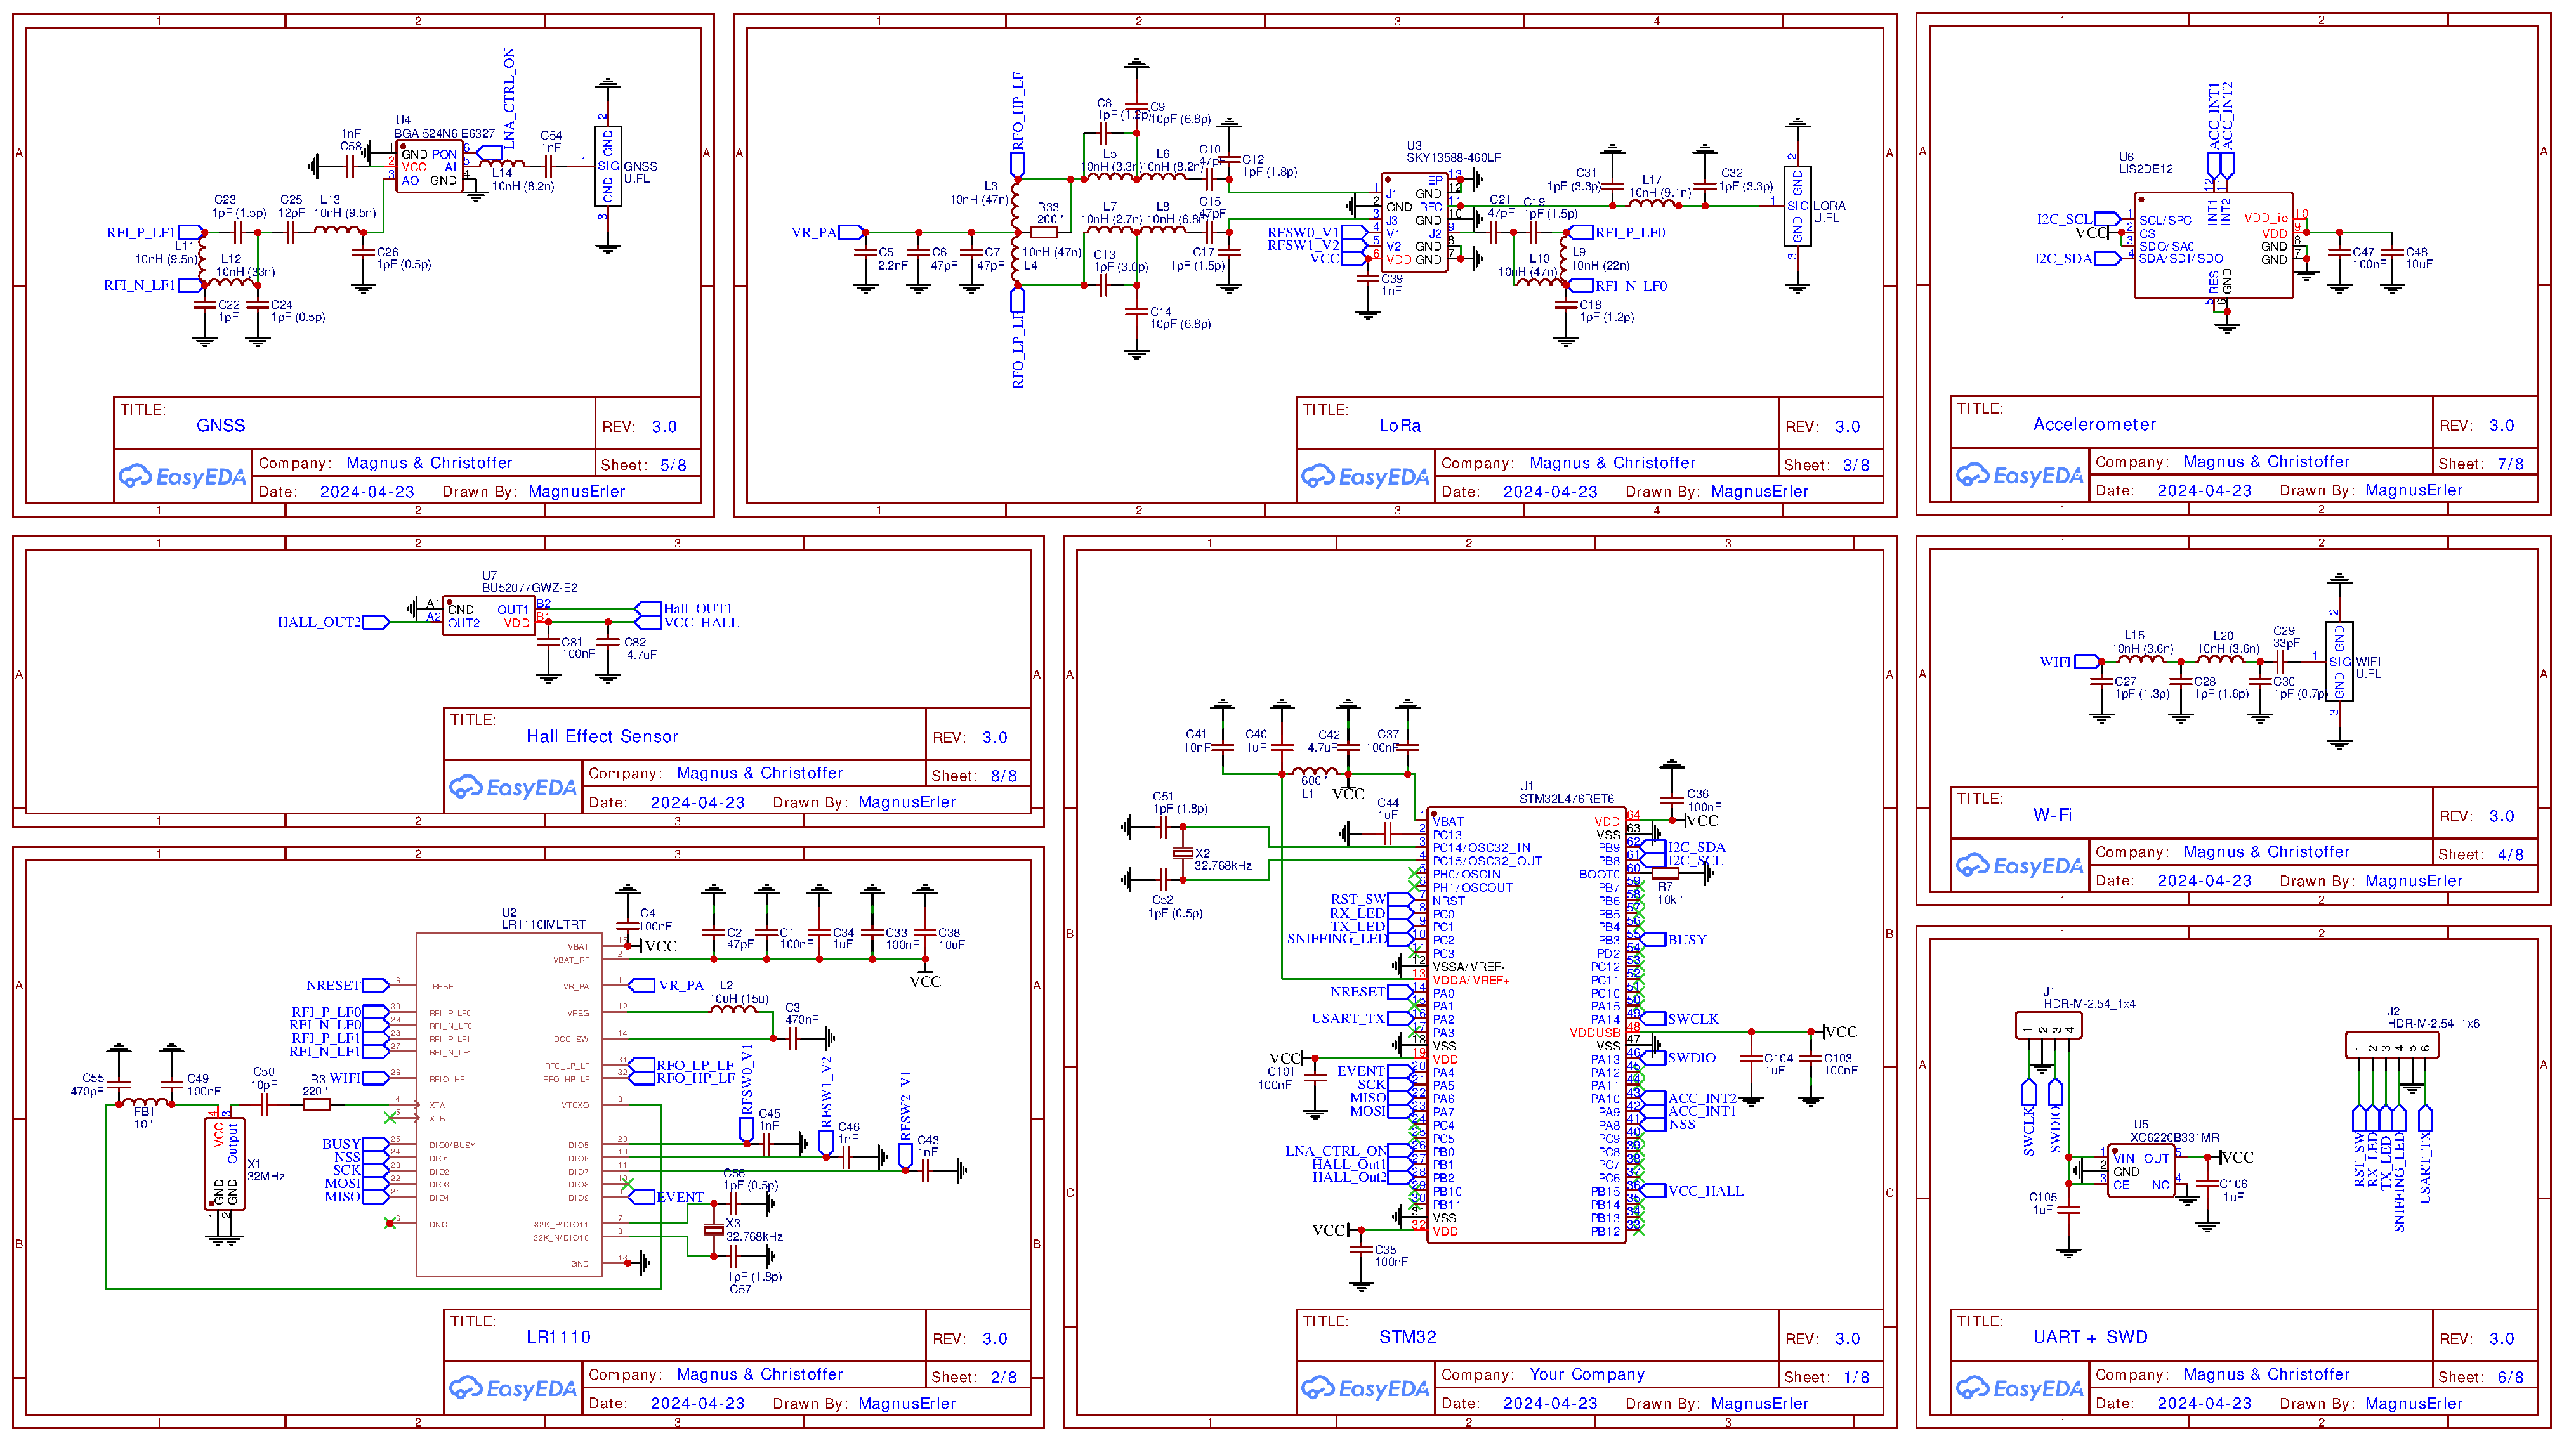
\includegraphics[width=1.38\textwidth]{figures/Schematic.pdf}
        \caption{Overview of the final schematic.}
    \end{figure}
\end{landscape}

\begin{landscape}
    \subsection{PCB} \label{app:PCB}
    \begin{figure}[H]  
        \centering
        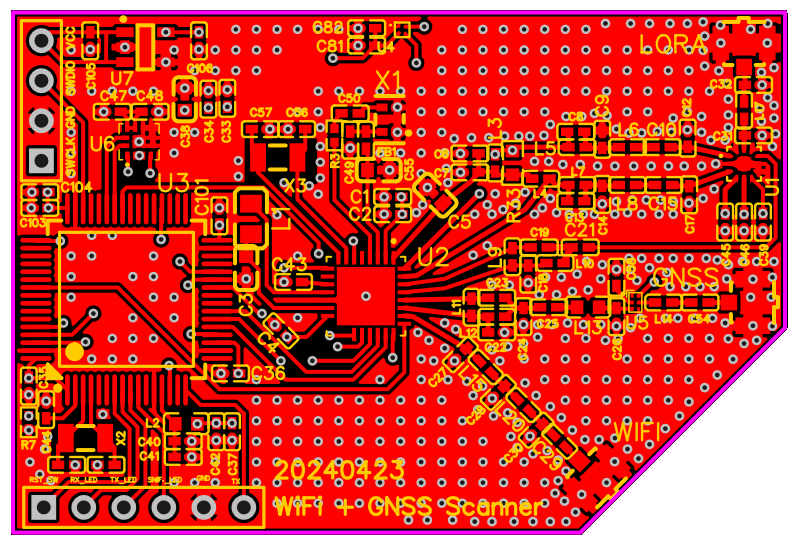
\includegraphics[width=1\textwidth]{figures/PCB_v3.png}
        \caption{Overview of the final PCB.}
    \end{figure}
\end{landscape}

\begin{landscape}
    \subsection{3D view} \label{app:3DView}
    \begin{figure}[H]  
        \centering
        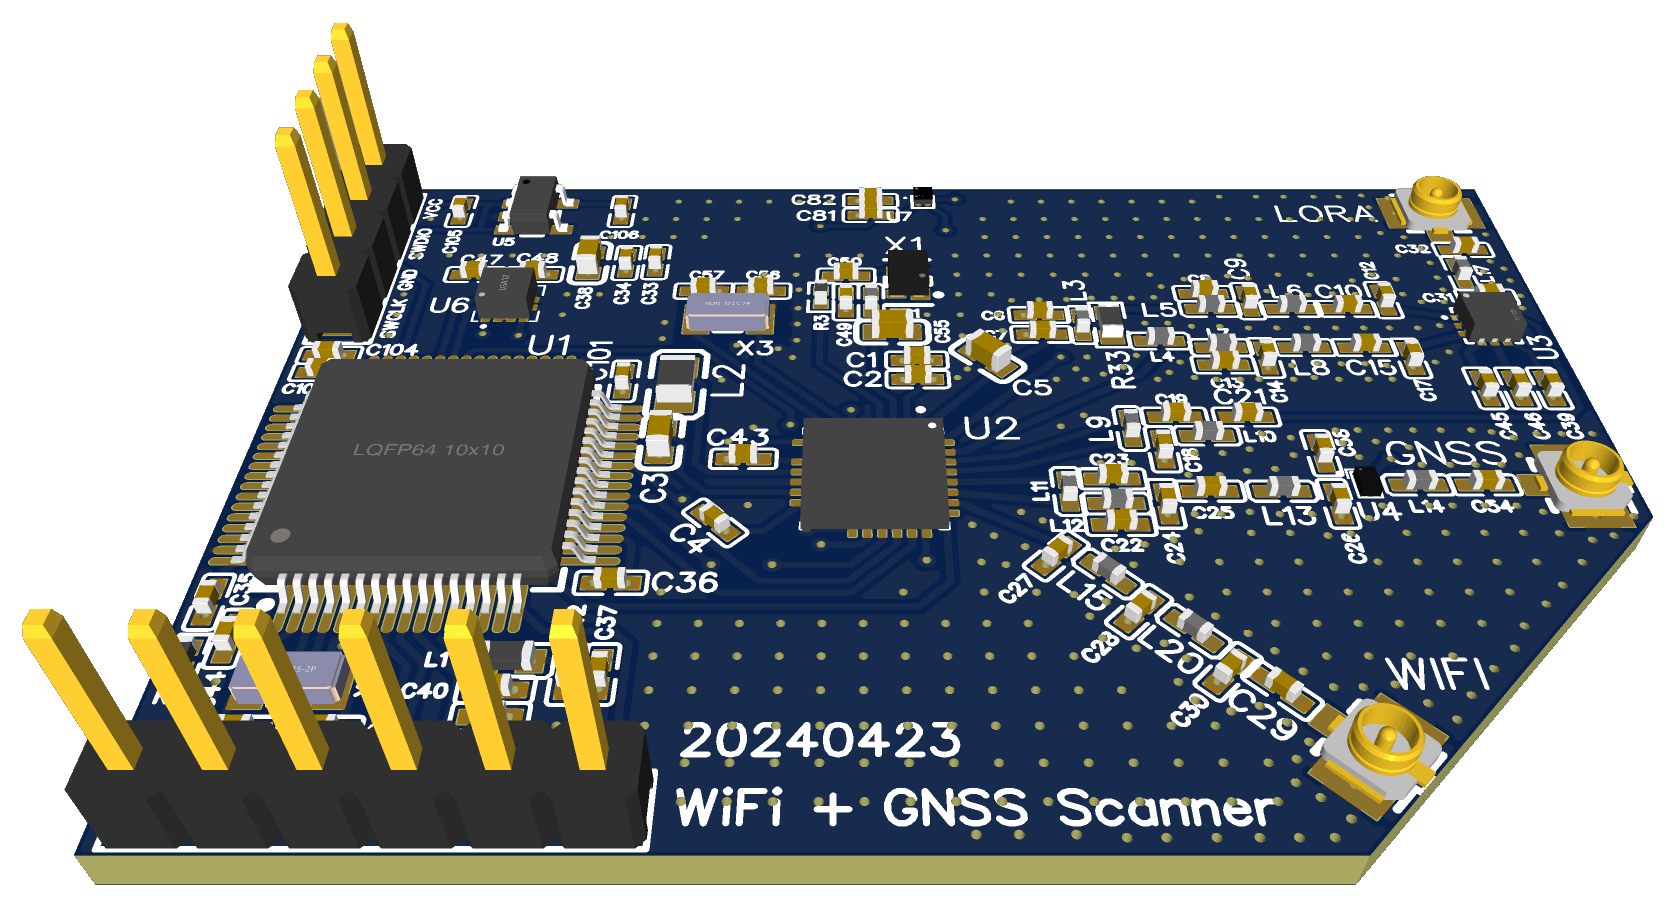
\includegraphics[width=1.38\textwidth]{figures/PCB_v3_3D.png}
        \caption{3D view of the final PCB.}
    \end{figure}
\end{landscape}

\end{appendices}

\end{document}
